\documentclass{lib/uekthesis}
\usepackage{lib/uekthesis}



%####################################################################
% INFORMACJE O PRACY DYPLOMOWEJ
%####################################################################

% tytuł pracy dyplomowej
\globalFullTitle{Gry jako medium do wywołania określonych emocji - porównanie gier wideo i gier z wykorzystaniem wirtualnej rzeczywistości}

% typ pracy, promotor
\globalThesisType{Praca magisterska}
\globalUnderTheSupervisonOf{Promotor}
\globalSupervisor{Prof. UEK dr hab. Grażyna Paliwoda-Pękosz}

% autor pracy i numer indeksu
\globalFullAuthor{Bartłomiej Hałdaś}
\globalAuthorID{Nr albumu: 192991}

% kierunek i specjalność studiów
\globalDegreeprogramme{Kierunek: Informatyka stosowana\\Specjalność: Systemy inteligentne}

% nazwa uniwersytetu
\globalFullUniversity{Uniwersytet Ekonomiczny w Krakowie}

% wydział, kolegium, instytut
\globalDepartment{Kolegium Nauk o Zarządzaniu i Jakości\\Instytut Zarządzania}

% miejscowość i rok
\globalCity{Kraków}
\globalYear{2020}



%####################################################################
% STRUKTURA PRACY DYPLOMOWEJ
%####################################################################

\begin{document}

% strona tytułowa
\titlepages

% spis treści
\tableofcontents

% rozdziały pracy 
\chapter*{Wstęp}
\label{chap:wstep}
\addcontentsline{toc}{chapter}{Wstęp}

Komputery nie służą już człowiekowi tylko jako narzędzie pracy z wysoką mocą obliczeniową, ale także dostarczają rozrywki wysokiej jakości bez potrzeby wychodzenia z domu. Gry pozwalają na aktywne doświadczenie, które może wyzwolić więcej emocji, a co za tym idzie więcej rozrywki niż media pasywne, dzięki narzędziom wykorzystywanym przez ich projektantów i twórców. 

Ludzie doświadczają rozmaitych emocji podczas grania w gry i jest to główny powód, który przyciąga miliardy graczy przed monitory w ciągu każdego roku. Gry wywołują różne stany emocjonalne u odbiorcy - różne typy gier są więc popularne wśród różnych odbiorców. Nie ma uniwersalnego doświadczenia, które zaspokoiłoby potrzeby każdego gracza, ale wszystkie pozycje mają wspólny mianownik, a mianowicie wywołanie konkretnego stanu u odbiorcy. Żadne inne medium nie oferuje takiej mocy transformacji jednostki na poziomie indywidualnym i społecznym, co jest możliwe dzięki dużej immersji przy równoczesnej możliwości wcielenia się w postać. Projektanci gier nadal przesuwają granice, pozwalając na coraz lepszą eksplorację świata oraz postaci, w które wciela się gracz.

Celem niniejszej pracy jest przybliżenie czytelnikowi czym jest technologia wirtualnej rzeczywistości (ang. Virtual Reality - VR), opisanie procesu powstania emocji oraz narzędzi wykorzystywanych do ich wywołania w grach oraz zbadanie jakimi zdolnościami do wywołania konkretnych emocji cechują się gry VR i gry wideo.  W toku badań własnych autora pracy udzielone zostaną odpowiedzi na następujące pytania badawcze: 

\begin{enumerate}
   \item Jaka jest charakterystyka graczy preferujących gry wideo, a jaka preferujących gry VR?
   \item Czym charakteryzuje się rozgrywka w gry typu VR, a czym w gry wideo?
   \item Czy emocje w grach są pożądane z perspektywy graczy oraz jaki jest związek pomiędzy platformą a wywołanymi emocjami?
\end{enumerate}

W tym celu przeprowadzono badania za pomocą kwestionariusza ankiety wśród osób mających styczność z grami wideo oraz technologią wirtualnej rzeczywistości.

Praca składa się z czterech rozdziałów. W pierwszym rozdziale scharakteryzowana zostaje technologia wirtualnej rzeczywistości, przybliżona zostaje jej historia oraz ewolucja na przestrzeni lat. Drugi rozdział definiuje pojęcie emocji, przedstawia jej funkcje oraz opisuje przebieg jej powstania u człowieka poprzez omówienie całego procesu: od oceny poznawczej aż po wykonanie działania. W kolejnym rozdziale zaprezentowano klasyfikację emocji oraz ukazanie jej związku z grami. Szczegółowo opisane zostają narzędzia wykorzystywane do wywołania emocji w grach oraz różnice między grami a innymi mediami pod względem wywołania emocji. W rozdziale czwartym zaprezentowano wyniki badań autora pracy. Scharakteryzowana została grupa badawcza, przedstawiono i przedyskutowano wyniki badań oraz udzielono odpowiedzi na sformułowane powyżej pytania badawcze.
\chapter{Wirtualna rzeczywistość}
\label{chap:pierwszy}



%-------------------------------------------------------
\section{Wprowadzenie}

Interfejs, bo tak nazwana jest płaszczyzna, na której dochodzi do komunikacji między człowiekiem a komputerem, przez wiele lat przechodziła ewolucje – począwszy od wiersza poleceń, poprzez interfejs graficzny, a skończywszy na bezpośredniej komunikacji na poziomie mózg-komputer. Użytkownicy pierwszych interfejsów musieli ówcześnie posiąść wiedzę na temat ich obsługi, gdzie przykładem może być konieczność zaznajomienia się ze składnią tekstową i komendami wykorzystywanymi w danym systemie operacyjnym. Dziś coraz częściej używane są komunikaty przekazane przez człowieka w naturalny i intuicyjny sposób, takie jak gesty wykonywane na ekranach dotykowych smartfonów palcami dłoni, komendy głosowe oraz gesty wykonywane przy pomocy ciała, rozpoznawalne przez kamery i czujniki ruchu  \citep{virtualtech, virtualspeech}.

Za finalny etap ewolucyjny  uważa się całkowitą naturalizację interfejsu – co można częściowo zaobserwować na przykładzie wirtualnej rzeczywistości. Pozwala ona na skrócenie dystansu pomiędzy maszyną a człowiekiem dzięki rozszerzeniu jego zmysłów: słuchu, dotyku i wzroku przy wykorzystaniu technologii informatycznej co pozwala na wykreowanie pewnej wizji rzeczywistości, jednakże w świecie wirtualnym. W ciągu następnych dekad możemy spodziewać się znaczących zmian w naszych działaniach związanych z pracą, rozrywką i komunikacją, a wszystko dzięki rozwojowi wirtualnej rzeczywistości \citep{virtualspeech}.



\section{Definicja, części składowe i systematyzacja wirtualnej rzeczywistości}

Wirtualna rzeczywistość zdefiniowana pod względem funkcjonalności to świat syntetyczny i niestatyczny, czyli taki, który reaguje na dane wejściowe użytkownika - gesty czy polecenia słowne. To z kolei, definiuje kluczową cechę wirtualnej rzeczywistości jaką jest interaktywność w czasie rzeczywistym. Interaktywność oraz siła z jaką VR absorbuje uwagę użytkownika, przyczyniają się do stworzenia uczucia ``zanurzenia'' w tymże świecie, czyli immersji \citep{virtualtech}.

Z powyższego opisu jasno wynika, że rzeczywistość wirtualna jest zarówno interaktywna (ang. interactive) jak i wciągająca (ang. immersive). Istnieje jednak trzecia składowa, bez której VR nie miałoby racji bytu, czyli ludzka wyobraźnia (ang. imagination). Zakres, w jakim aplikacja jest w stanie rozwiązać konkretny problem, czyli stopień, w którym symulacja działa prawidłowo, zależy więc w dużej mierze od ludzkiej wyobraźni. Rzeczywistość wirtualna jest zatem zintegrowanym trio immersji-interakcji-wyobraźni (ang. immersion, interaction, imagination), tak jak to pokazano na rysunku \ref{fig:triangle}, czyli trójkącie trzech ``I'' wirtualnej rzeczywistości \citep{virtualtech}.


\begin{figure}[h]
	\centering
	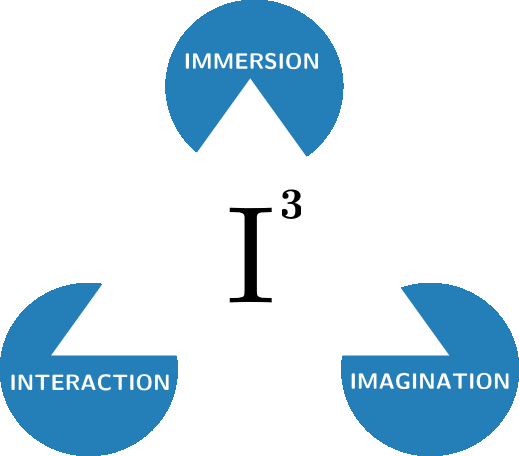
\includegraphics[width=0.6\textwidth]{images/triangle.png}
	\caption{Trzy składowe wirtualnej rzeczywistości.}
	\caption*{Źródło: \citep[s.~5]{virtualtech}.}
	\label{fig:triangle}
\end{figure}

Składowa jaką jest wyobraźnia, odnosi się do zdolności umysłu do postrzegania zasugerowanych, lecz nieistniejących rzeczy. Stąd trójkąt na rysunku 1 jest widoczny dla czytelnika, ale istnieje tylko w jego wyobraźni \citep{virtualtech}.

W celu ujednolicenia, każde kolejne odniesienie do wirtualnej rzeczywistości będzie bazowało na następującej definicji. Rzeczywistość wirtualna to immersyjna, interaktywna rzeczywistość symulowana komputerowo, która dzięki zaawansowanym urządzeniom wejścia i wyjścia tworzy złudzenie fizycznego środowiska, nie istniejącego w prawdziwym świecie fizycznym. Środowiska VR są zazwyczaj odcięte od tego świata w tym sensie, że cyfrowe środowiska, które powstają są całkowicie nowe - chociaż mogą być oparte na prawdziwych miejscach (takich jak szczyt Mount Everest) lub wymyślonych (takich jak podwodne miasto Atlantyda). Osoba korzystająca z wirtualnej rzeczywistości może rozglądać się po sztucznym świecie, poruszać się po nim, a także wchodzić w interakcję z wirtualnymi funkcjami i przedmiotami \citep{virtualfor}.

Rzeczywistość wirtualna jest często używana jako pojęcie ogólne dla wszelkiego rodzaju doświadczeń mocno absorbujących uwagę użytkownika, w tym wielu powiązanych terminów, takich jak rzeczywistość rozszerzona (ang. augumented reality, AR), rzeczywistość mieszana (ang. mixed reality, MR)  i rzeczywistość rozszerzona (ang. extended reality, XR) \citep{virtualfor}. W celu wyjaśnienia, czym dokładnie jest wirtualna rzeczywistość i czym różni się od pochodnych jej technologii, zostaną one umieszczone na skali Paula Miligrama, nazwanej kontinuum wirtualności, którą przedstawia rysunek \ref{fig:continuum}.

\begin{figure}[h]
	\centering
	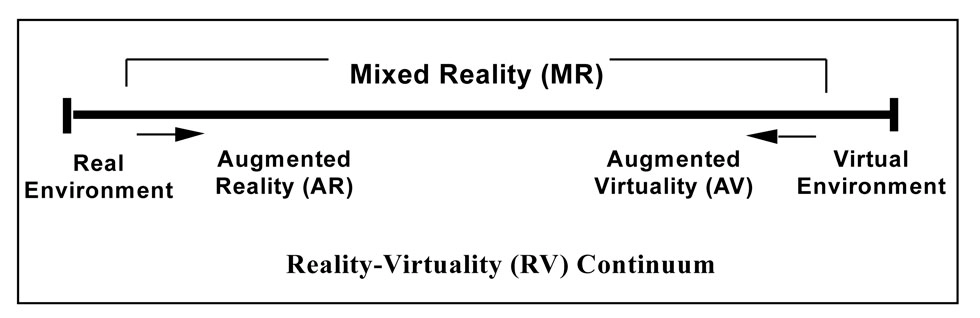
\includegraphics[width=1\textwidth]{images/2.spektrum.png}
	\caption{Kontinuum wirtualności.}
	\caption*{Źródło: \citep[s.~14]{virtualfor}.}
	\label{fig:continuum}
\end{figure}

Kontinuum wirtualności to skala używana do pomiaru poziomu rzeczywistości lub wirtualności konkretnych technologii. Na jednym końcu skali poziom jest w pełni realny, a na drugim całkowicie wirtualny. XR obejmuje pełne spektrum tej skali. Warto dodać, że MR oraz AR zostały rozdzielone, pomimo tego, że często określeń tych używa się synonimicznie. Niniejszy rozdział skupiać się będzie natomiast na głównych dwóch obszarach: VR i AR, które pokrywają większość scenariuszy związanych z rozszerzoną rzeczywistością.  Wirtualna rzeczywistość będzie używana w stosunku do kombinacji sprzętu i oprogramowania, które tworzy całkowicie nowe, cyfrowe symulacje. Natomiast rzeczywistość rozszerzona odnosić się będzie do dowolnego, istniejącego środowiska fizycznego jakie zostało wzbogacono o elementy cyfrowe, które z kolei nie muszą z nim bezpośrednio oddziaływać ani być interaktywne \citep{virtualfor}.

Rzeczywistość rozszerzona AR to jeden ze sposobów oglądania prawdziwego świata w sposób bezpośredni lub za pomocą urządzeń elektronicznych, takich jak kamera, która tworzy wizualizację świata fizycznego i ``rozszerza'' go za pomocą generowanych komputerowo danych graficznych, dźwiękowych i filmowych. AR różni się od VR tym, że AR powiększa istniejącą już fizycznie scenę o dodatkowe elementy, zamiast tworzyć całkowicie nową od podstaw. Pierwotnie uważano, że w AR dwa środowiska: fizyczne i syntetyczne nie mogą się ze sobą komunikować. W ostatnich latach definicja AR przybrała jednak inną formę i jest utożsamiana z rzeczywistością mieszaną, czyli taką, w której może zachodzić interakcja między światem rzeczywistym a cyfrowo rozszerzonym \citep{virtualfor}.

Porównanie zasady działania różnych typów rozszerzonej rzeczywistości przedstawia rysunek \ref{fig:vr-ar-mr}. Kolor zielony odwzorowuje obraz wirtualny, natomiast odcienie szarości przedstawiają świat fizyczny.


\begin{figure}[ht]
	\centering
	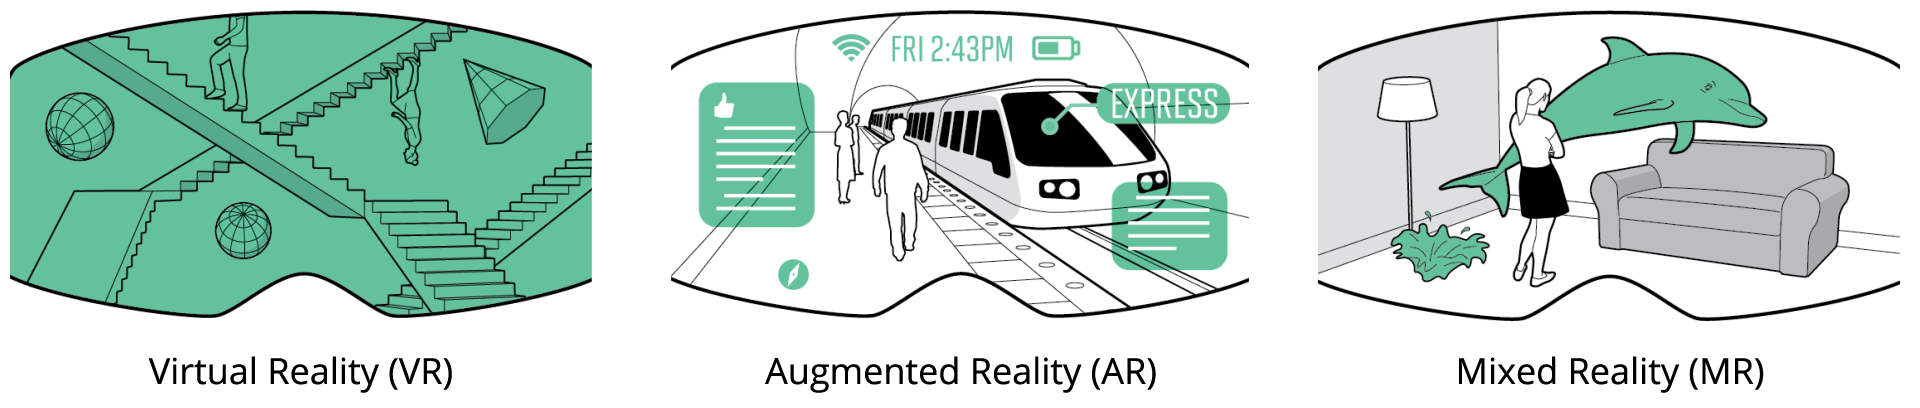
\includegraphics[width=1\textwidth]{images/1.xr-comparision.png}
	\caption{Porównanie VR, AR oraz MR.}
	\caption*{Źródło: https://www.cadcompany.nl/blog/vr-ar-en-mr-verschillen/}
	\caption*{Data dostępu: 15.02.2020.}
	\label{fig:vr-ar-mr}
\end{figure}

Rzeczywistość mieszana MR może przybrać różne formy i skłaniać się bardziej w stronę AR lub VR. Rzeczywistość mieszana, której podstawą jest AR, nie jest pasywnie nakładana na świat rzeczywisty, lecz zachowuje się jakby była częścią tego świata i wchodzi z nim w interakcje. Obiekty cyfrowe wyglądają tak, jakby istniały w prawdziwej przestrzeni. Przykładem może być umieszczona na stoliku do kawy cyfrowa rakieta, która rozpoczyna swoją misję kosmiczną lub cyfrowa piłka, która odbija się od ścian świata rzeczywistego. W innej wersji natomiast ukazuje się całkowicie cyfrowe środowisko lecz powiązane z otaczającymi użytkownika obiektami świata rzeczywistego, tak więc na przykład fizyczne, drewniane krzesła mogą mieć swoje odwzorowanie jako drzewa w cyfrowym świecie – jest to MR oparty na VR \citep{virtualfor}.

Rozszerzona wirtualność AV (z ang. Augumented virtuality), nazywana także połączoną rzeczywistością jest zasadniczo odwrotnością AR. Rozszerzona wirtualność dotyczy środowiska cyfrowego, w którym istnieje pewna integracja obiektów rzeczywistych poprzez strumieniowe przesyłanie video do środowiska wirtualnego lub tworzenia cyfrowej reprezentacji 3D istniejącego obiektu fizycznego \citep{virtualfor}.



%-------------------------------------------------------
\section{Ewolucja wirtualnej rzeczywistości}


%-------------------------------------------------------
\subsection{Narodziny}

Biorąc pod uwagę VR jako narzędzie do tworzenia iluzji – przeniesienia użytkownika w miejsce, w którym nie jest fizycznie to jako tego najwcześniejszą próbę możemy traktować 360 stopniowe malowidła ścienne lub panoramiczne obrazy z XIX wieku. Ich celem było wypełnienie całego pola widzenia obserwatora, sprawiając przy tym, że czuł się on ``zanurzony'' w wydarzeniu lub scenie oddanej na malowidle \citep{interactivemedia}.

Badania opublikowane w 1838 roku przez Charlesa Wheatstone’a wykazały, że ludzki mózg przetwarza dwa dwuwymiarowe obrazy z każdego oka w jeden, pojedynczy obiekt o trzech wymiarach. Stąd oglądanie dwóch zdjęć (jedno widoczne dla jednego oka, a drugie – podobne lecz nieidentyczne dla drugiego) za pomocą stereoskopu zapewniało użytkownikowi poczucie głębi i zanurzenia. Późniejszy rozwój popularnego stereoskopu View-Master opatentowanego w 1939 roku, dało początek dzisiejszym goglom VR \citep{interactivemedia}.

Wirtualna rzeczywistość choć dopiero teraz zyskuje na popularności, nie jest wynalazkiem XXI wieku, a jej historia sięga lat 50 ubiegłego stulecia. Za ojca VR uważany jest operator filmowy Morton Heiling, który to w 1962 roku zaprezentował maszynę o nazwie ``Sensorama'', którego schemat widnieje na rysunku \ref{fig:sensorama1}, a zdjęcie zostało przedstawione na rysunku \ref{fig:sensorama2}.  Było to urządzenie mechaniczne, którego zadaniem było symulowanie jazdy motocyklem przez Nowy Jork \citep{determinants}. Doświadczenie to polegało na jeździe wyimaginowanym motorem podczas oglądania krótkich ujęć filmów z ulic Nowego Jorku. W celu zwiększenia realności całego doświadczenia, symulowano podmuchy wiatru, zmiany kierunku jazdy, hałas oraz zapachy spotykane w mieście – od spalin po nowojorską pizzę, w zależności od miejsca, w jakim aktualnie znajdował się użytkownik. W systemie Sensorama brakowało jednak głównego elementu nowoczesnego systemu rzeczywistości wirtualnej: reakcji opartej na działaniach użytkownika \citep{virtualdev}.


\begin{figure}[ht]
    \centering
    \begin{minipage}{0.45\textwidth}
        \centering
        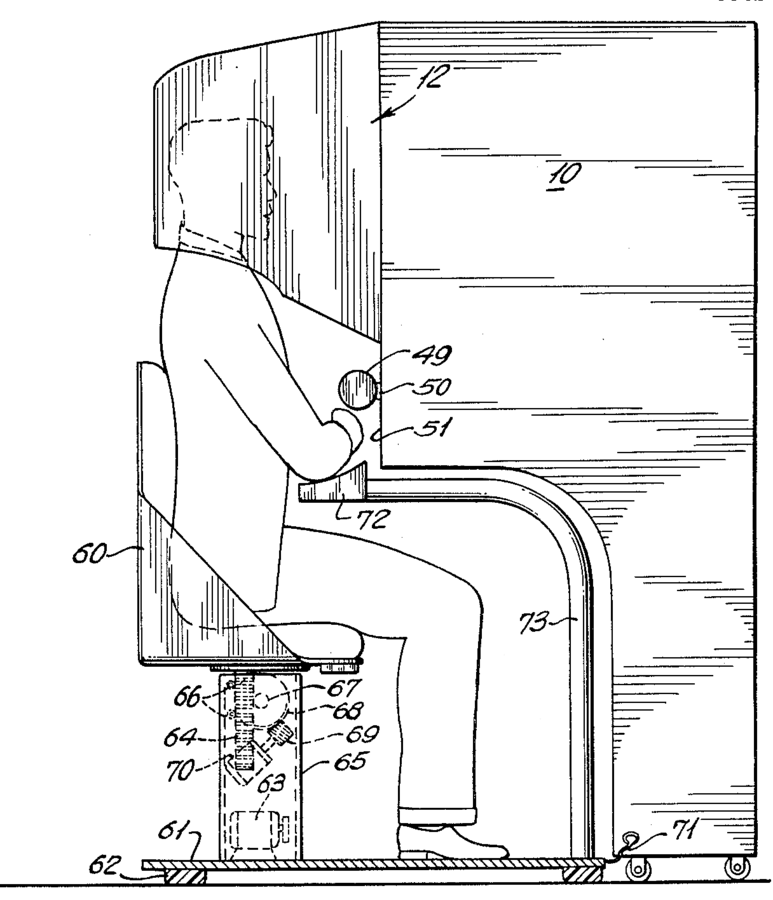
\includegraphics[width=0.9\textwidth]{images/sensorama1.png} % first figure itself
        \caption{Schemat Sensoramy w przekroju bocznym (zdjęcie z patentu USA nr #3050870).}
        \caption*{Źródło: https://smattes.com/article
        /47/sensorama}
        \caption*{Data dostępu: 15.02.2020.}
        \label{fig:sensorama1}
    \end{minipage}\hfill
    \begin{minipage}{0.45\textwidth}
        \centering
        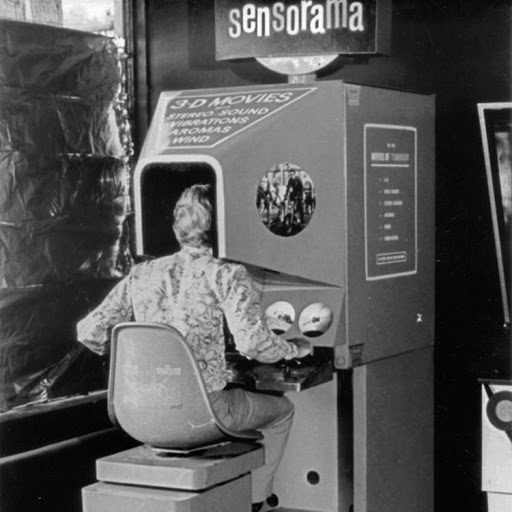
\includegraphics[width=0.9\textwidth]{images/sensorama2.jpg} % second figure itself
        \caption{Sensorama - pierwsze urządzenie wykorzystujące VR.}
        \caption*{Źródło: https://www.researchgate.net
        /figure/Sensorama-From-web-page-
        InventorVR-retrieved-in-March-2014-from\_fig1\_263388241}
        \caption*{Data dostępu: 15.02.2020.}
        \label{fig:sensorama2}
    \end{minipage}
\end{figure}


%-------------------------------------------------------
\subsection{Rozwój}

Krótko po wynalezieniu Sensoramy, Heilig opatentował również maskę Telesphere, pierwszy w historii wyświetlacz montowany na głowie HMD (ang. head-mounted display), czyli tak zwany hełm wideo, który zapewniał stereoskopowy obraz 3D i dźwięk stereo. Zestaw ten był nadal nieinteraktywny, choć zewnętrznie przypominał dzisiejsze okulary VR \citep{website:virtualspeech}.

W roku 1968 Ivan Sutherland, profesor Harvardu w dziedzinie informatyki, wynalazł pierwszy interaktywny hełm wideo, który był podłączony do komputera. System Sutherlanda to duży sprzęt, podwieszany przy suficie, który nosił nazwę ``Miecz Damoklesa''. Obejmował on hełm wideo oraz elementy, które mechanicznie śledziły głowę za pomocą szpulowych zwijanych kabli oraz program komputerowy, który w prosty sposób w formie trójwymiarowej generował prymitywne pokoje lub obiekty szkieletowe jak na przykład cząsteczka wody.  Sutherland w późniejszym czasie opracował zaawansowany sprzęt do renderowania grafiki w czasie rzeczywistym dla społeczności pilotów korzystających z symulatorów lotów, już jako  współzałożyciel Evans i Sutherland Computer Corporation (E&S) \citep{virtualdev}.


Po demonstracji Sutherlanda w laboratoriach uniwersyteckich, instytucjach rządowych i wojskowych, a później w sektorze komercyjnym, podjęto szereg prac badawczo-rozwojowych. W społeczności akademickiej badacz z University of Wisconsin, Myron Krueger eksperymentował z rozszerzoną rzeczywistością, czego wynikiem było powstanie systemu nazwanego ``Videoplace''. Systemy Kruegera również różniły się od pracy Sutherlanda tym, że wykorzystywał sygnały wejściowe z kamery wideo do śledzenia ruchów użytkownika. Videoplace było miejscem, w skład którego wchodziły zaciemnione pomieszczenia z zainstalowanymi na ścianach ekranami wideo, które otaczały użytkownika. Odbiorcy mogli zobaczyć wygenerowane przez komputer sylwetki naśladujące ich ruchy i działania - ruchy użytkowników były rejestrowane w kamerze i przenoszone na wirtualną postać. Ponadto użytkownicy różnych pokoi mogli wchodzić w interakcje z innymi użytkownikami w wirtualnym świecie, co powoli prowadziło do wniosków, że komunikacja w wirtualnym świecie jest możliwa, nawet jeśli dwie osoby nie są fizycznie blisko \citep{website:virtualspeech}.


W czasie, gdy Ivan Sutherland pracował nad projektem „Miecz Damoklesa”, inżynier wojskowy Thomas Furness opracowywał swój prywatny projekt - ``Super Kokpit''. Furness kontynuował prace nad projektem do lat osiemdziesiątych, w wyniku czego kokpit szkoleniowy był w stanie wyświetlać wygenerowane komputerowo mapy 3D, zdjęcia w podczerwieni i obrazy radarowe, a także dane samolotu w przestrzeni 3D w czasie rzeczywistym \citep{website:digitaltrends}.

W roku 1978 Massachusetts Institute of Technology (MIT) opracowało Aspen Movie Map, która znacząco przypominała dzisiejszą funkcję ``street view'' oferowaną przez Google Maps. Program ten pozwolił użytkownikowi na wirtualny spacer przez miasto Aspen (Kolorado) w trzech trybach: letnim, zimowym i wyświetlającym wielokąty. Doświadczenie to zostało stworzone na podstawie zdjęć z samochodu jadącego przez miasto. Chociaż projekt ten nie wykorzystywał komponentu hełmu wirtualnego,  w sposób innowacyjny wykorzystano interaktywność z perspektywy pierwszej osoby i ukazano w jak prosty sposób VR można wykorzystać do ``wirtualnego przeniesienia'' ludzi w inne miejsce na Ziemi \citep{website:digitaltrends}.

Rękawice do śledzenia palców dla VR, zwane rękawiczkami ``Sayre'' zostały wynalezione przez Daniela Sandina i Thomasa DeFanti. Rękawice były podłączone do systemu komputerowego i monitorowały ruchy dłoni za pomocą emiterów światła i fotokomórek w palcach rękawic. Kiedy użytkownik poruszał palcami, ilość światła padającego na fotokomórkę zmieniała się, co następnie przekształcało ruchy palców w sygnały elektryczne. Był to prekursor ``rękawic danych'', które stały się w późniejszym czasie ważną częścią wczesnej rzeczywistości wirtualnej \citep{website:virtualspeech}.

Pomimo prężnego rozwoju VR wciąż nie było terminu opisującego tę dziedzinę. Wszystko zmieniło się w 1987 roku, gdy Jaron Lanier, założyciel laboratorium programowania wizualnego (VPL), wymyślił termin ``rzeczywistość wirtualna''. W późniejszym czasie, dzięki swojej firmie VPL Research Jaron opracował gamę sprzętu do rzeczywistości wirtualnej, w tym Dataglove (wraz z Tomem Zimmermanem) i montowany na głowie wyświetlacz  EyePhone. Była to pierwsza firma, która sprzedawała gogle oraz rękawice do obsługi wirtualnej rzeczywistości. Miało to znaczący wpływ na rozwój w dziedzinie dotykowej rzeczywistości \citep{website:learng2, interactivemedia}. Rysunek \ref{fig:eyephone} przedstawia rękawice Dataglove oraz headset Eyephone podczas użytkowania.

\begin{figure}[ht]
	\centering
	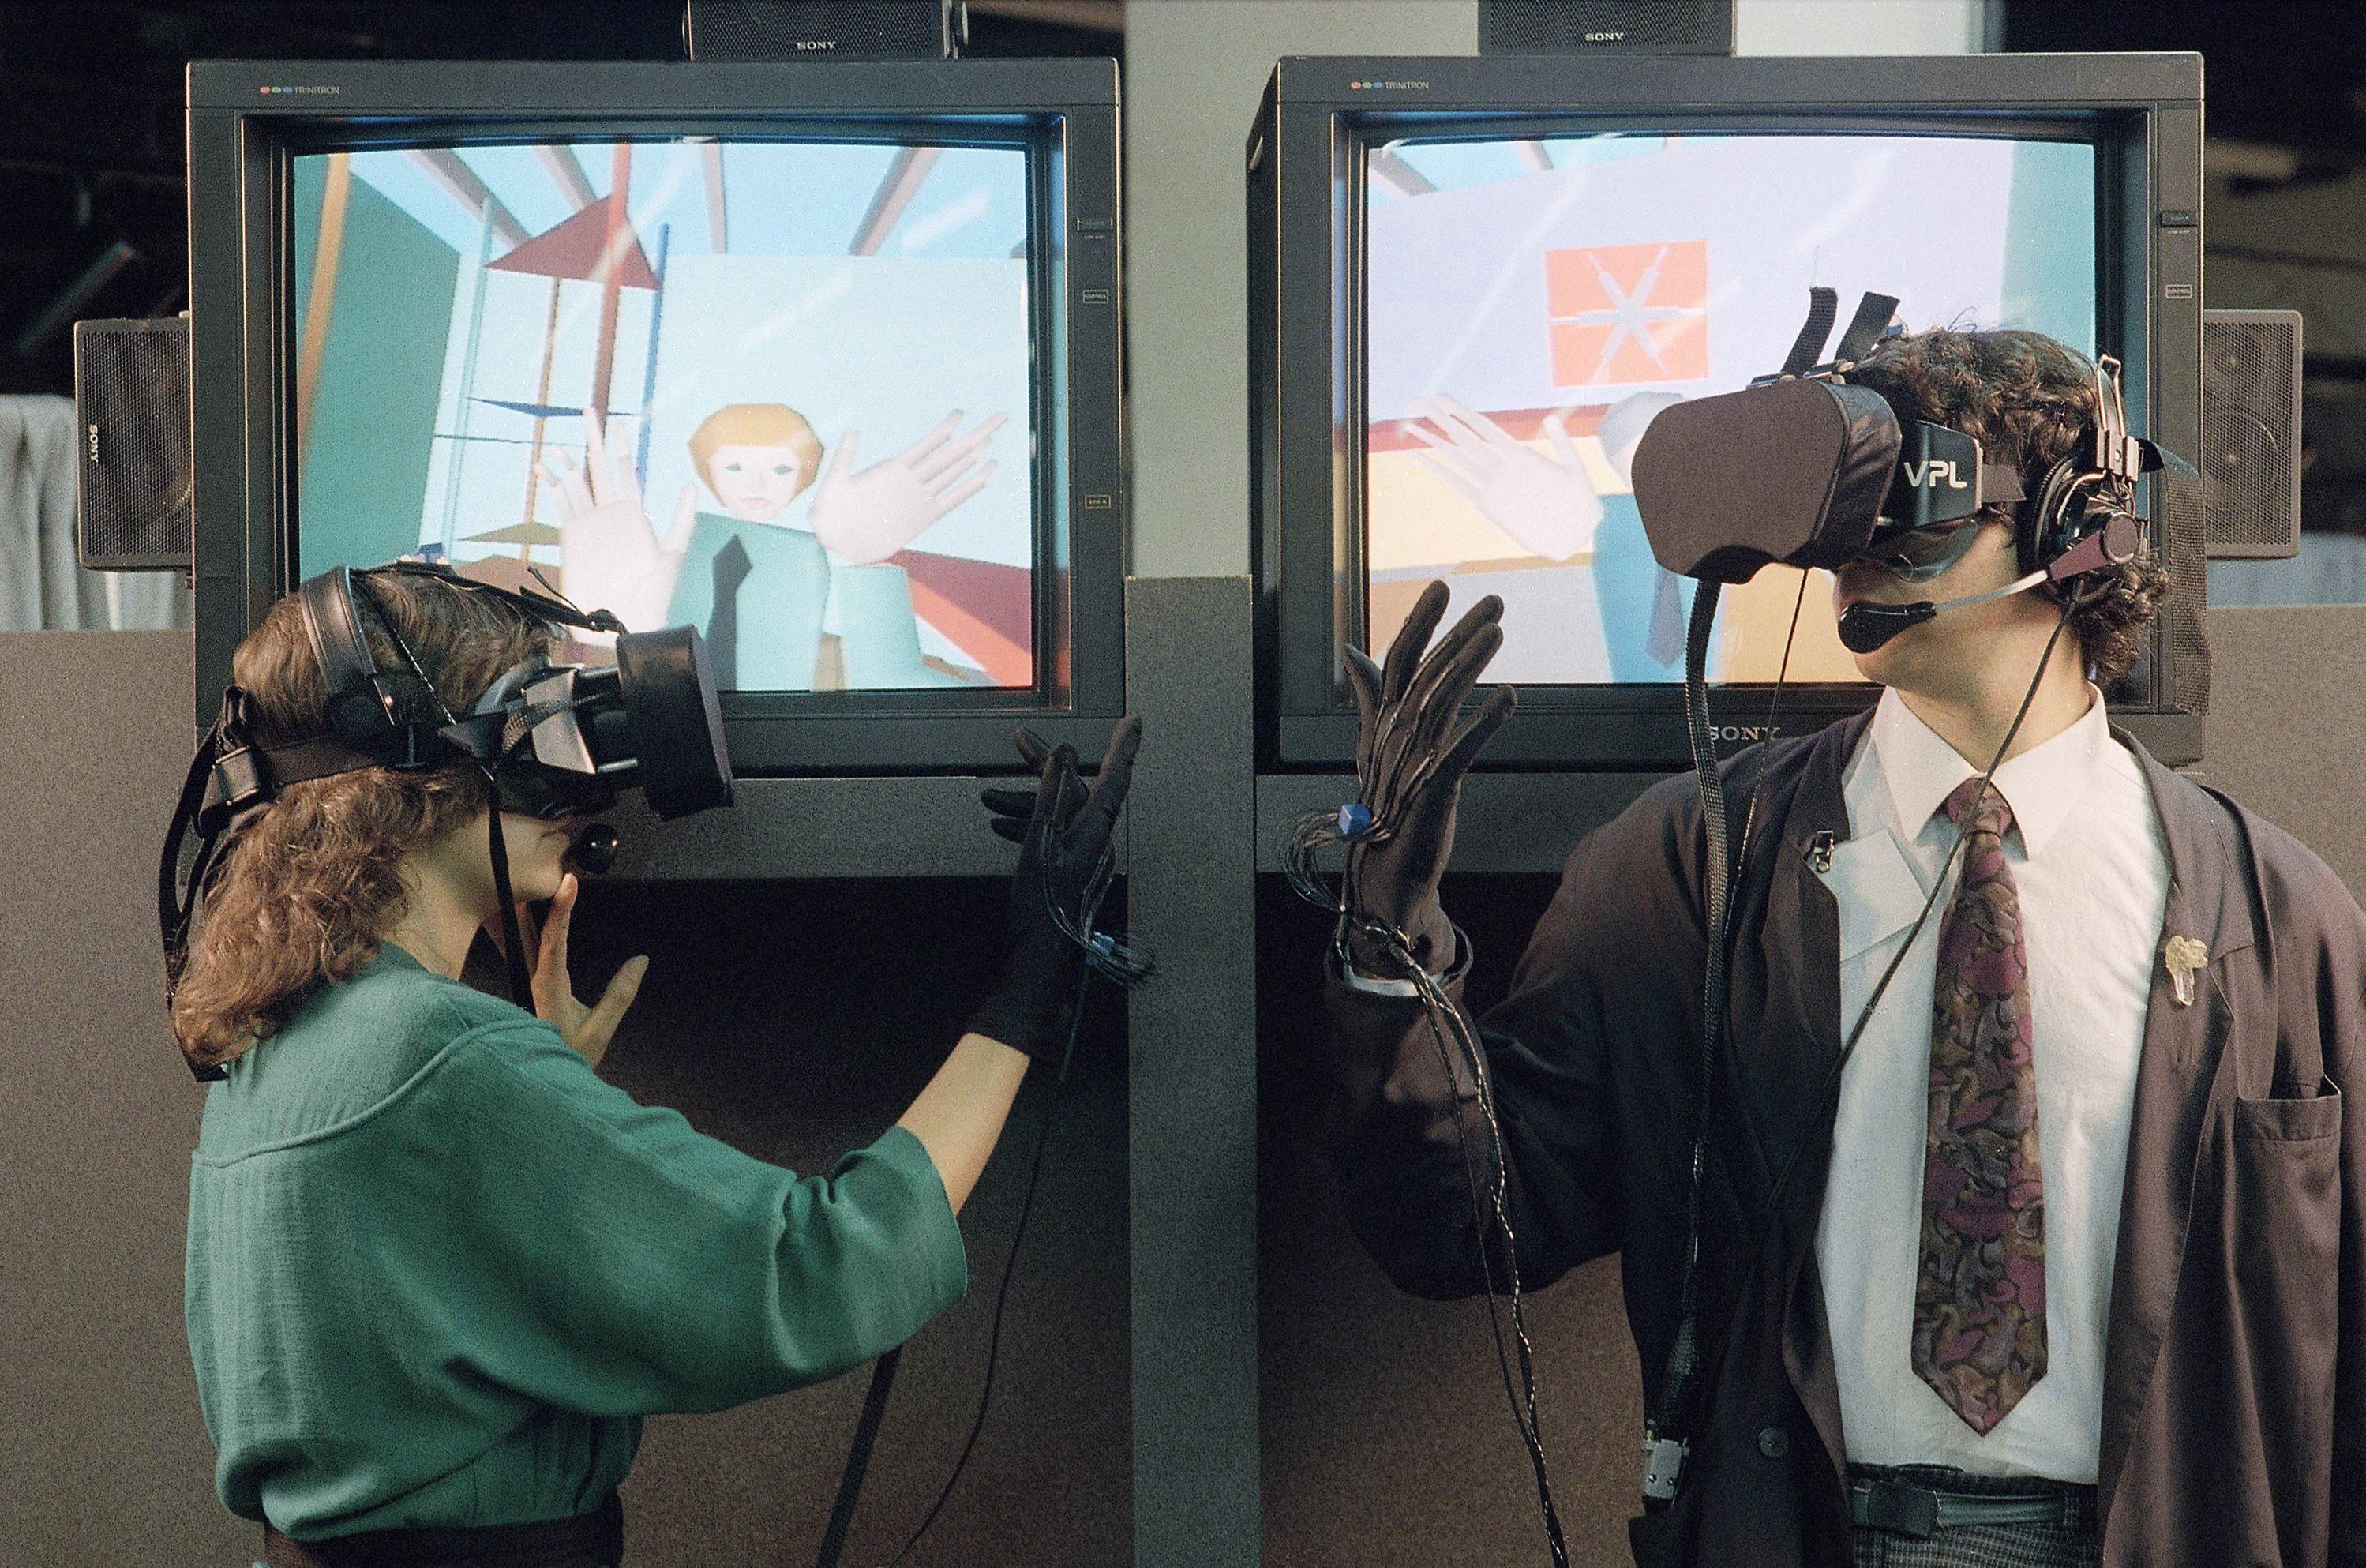
\includegraphics[width=0.7\textwidth]{images/jaron.jpg}
	\caption{Rękawice Dataglove oraz headset Eyephone w trakcie użycia.}
	\caption*{Źródło: https://flashbak.com/jaron-laniers-eyephone-head
	-and-glove-virtual-reality-in-the-1980s-26180/}
	\caption*{Data dostępu: 20.02.2020.}
	\label{fig:eyephone}
\end{figure}

Rok 1991 był przełomowy dla systemów VR dostarczających rozrywkę. Grupa Virtuality zaczęła dystrybuować automaty do gier VR o nazwie ``Virtuality'', w których gracze mogli grać w świecie gier 3D. Był to pierwszy masowo produkowany system rozrywki VR. Virtuality zawierała stereoskopowe okulary VR, które generowały obrazy 3D w czasie rzeczywistym. Niektóre z maszyn mogły być podłączone wspólnie, pozwalając przy tym na grę w trybie wieloosobowym \citep{website:virtualspeech}.

W 1993 SEGA ogłosiła, że pracuje nad zestawem słuchawkowym SEGA VR, który będzie dostępny dla ogółu społeczeństwa. Ten zestaw słuchawkowy miał być przeznaczony do gier zręcznościowych i konsoli Mega Drive. Wyglądał jak przyłbica dzięki wpływom popularnych wtedy filmów, takich jak RoboCop. W wizjerze umieszczono wyświetlacze LCD, a także słuchawki stereo i czujniki do śledzenia ruchu głowy. Jednak projekt ten nigdy nie został wydany, choć stworzono dla niego cztery gry. Jednym z wyjaśnień jakie ogłosiła firma SEGA, była ich obawa przed utratą zdrowia użytkowników, ponieważ efekt VR był zbyt realistyczny. Wydaje się to jednak mało prawdopodobne ze względu na ograniczoną moc obliczeniową w tamtych latach \citep{website:virtualspeech}.

W roku 1997 rozpoczęto terapie w leczeniu zespołu stresu pourazowego (ang. Posttraumatic Stress Disorder, PTSD) u weteranów wojennych. Do dnia dzisiejszego jest to nadal jeden z kluczowych obszarów leczenia i badań PTSD. Technologia VR dała terapeutom niezrównaną kontrolę nad tym, co pacjenci widzą i czego doświadczają \citep{interactivemedia}.


%-------------------------------------------------------
\subsection{Lata współczesne i prognozy na przyszłość}

Prawdziwy przełom nastąpił w roku 2010. Przedsiębiorca Palem Luckey był zawiedziony zestawami VR dostępnymi na rynku. Według jego opinii były zbyt drogie, ciężkie oraz miały małe pole widzenia, a opóźnienia miedzy interakcją użytkownika a odpowiedzią komputera były zbyt długie. Luckey zbudował serie prototypów zestawów VR, koncentrując się przy tym na stworzeniu taniego zestawu o niskim opóźnieniu, ale z dużym polem widzenia oraz wygodnym w użytku. Jego jednostka szóstej generacji została nazwana Oculus Rift Development Kit 1 i zaoferował ją na platformie Kickstarter, pozwalającej na finansowanie przez użytkowników projektów z różnych dziedzin życia. Zbiórka pieniędzy na rzecz projektu odniosła ogromny sukces, przynosząc 2,4 miliona dolarów, prawie 980 procent pierwotnego celu. Co ważniejsze, kampania Kickstarter przyczyniła się do wzrostu zainteresowania VR na rynku konsumenckim do rekordowego poziomu \citep{virtualfor}. Porównanie pierwszej i najnowszej wersji zestawu Oculus przedstawiono na rysunku \ref{fig:rift} i rysunku \ref{fig:quest}.

\begin{figure}[ht]
    \centering
    \begin{minipage}{0.45\textwidth}
        \centering
        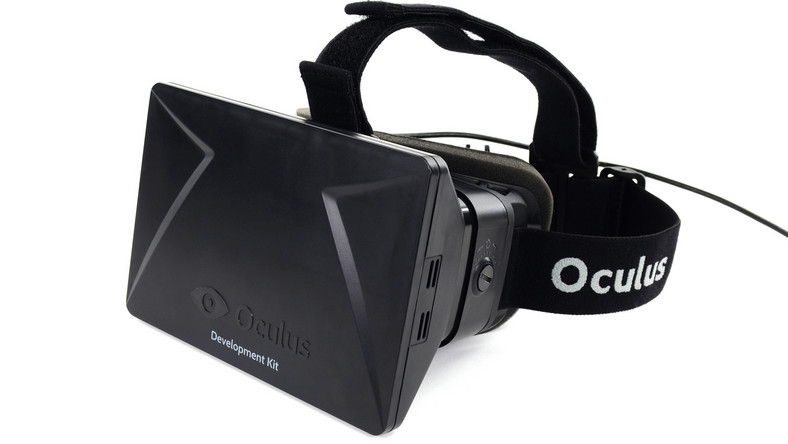
\includegraphics[width=0.9\textwidth]{images/oculusold.jpg} % first figure itself
        \caption{Zestaw Oculus Rift Development Kit 1 z roku 2010.}
        \caption*{Źródło: https://www.ifixit.com/Device
        /Oculus\_Rift\_DK1}
        \caption*{Data dostępu: 25.02.2020.}
        \label{fig:rift}
    \end{minipage}\hfill
    \begin{minipage}{0.45\textwidth}
        \centering
        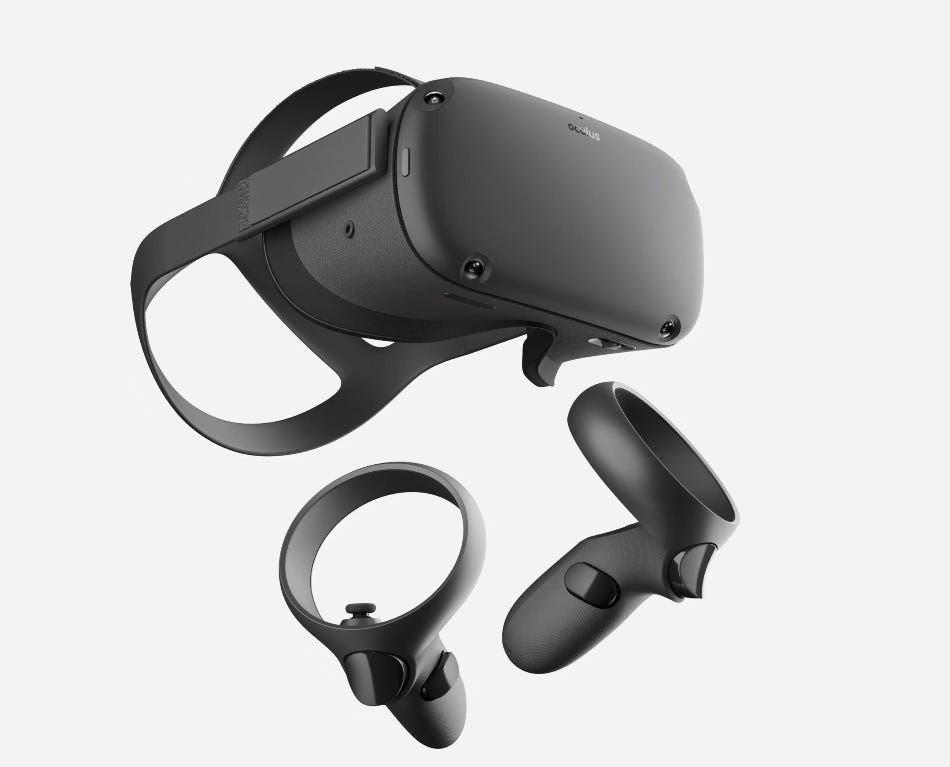
\includegraphics[width=0.9\textwidth]{images/oculusquest.jpg} % second figure itself
        \caption{Zestaw Oculus Quest z roku 2019.}
        \caption*{Źródło: https://i.insider.com/
        5df1222cfd9db23851669bd2?width=1100&
        format=jpeg&auto=webp}
        \caption*{Data dostępu: 25.02.2020.}
        \label{fig:quest}
    \end{minipage}
\end{figure}

Firma została zakupiona przez Facebook za 2 miliardy dolarów w 2014 roku. Decyzja Luckeya o sprzedaży firmy przed wysyłką prototypów do użytkowników, którzy zapłacili przez serwis Kickstarter wzbudziła kontrowersję, jednak był to dla historii VR decydujący moment, uznawany za przełomowy względem wzrostu popularności tej technologii \citep{virtualfor}.

Setki firm pracują nad własnymi zestawami VR: należą do nich liderzy rynku; wielkie koncerny takie jak HTC, Google, Apple, Amazon, Sony, Samsung oraz wiele innych, pomniejszych kompani. Prowadzi to do coraz większego popularyzowania tej technologii, jej szybkiego rozwoju przy jednoczesnym spadku cen, które są kluczowe dla rynku konsumenckiego i czynią  zaawansowaną technologię codziennym produktem w życiu człowieka. Dzisiejsze zestawy VR cechują się mobilnością i niewygórowanymi cenami, dzięki czemu mogą z nich skorzystać przeciętni użytkownicy innych powszechnie używanych technologii \citep{website:virtualspeech}.

Aktualne liczbę graczy ogółem na świecie szacuje się na ponad 2.5 miliarda, z czego gracze VR to tylko 171 milionów \citep{website:gameindustry, website:vrstats}. Liczba ta ciągle rośnie, a to za sprawą wciąż rozwijającej się technologii VR. Największą wadą VR jest brak rozbudowanych, wysokobudżetowych gier, lecz i to ulega zmianie. Wydanie jednej, dobrze przyjętej przez graczy produkcji może znacząco zmienić liczbę aktywnych graczy. Przykładem może być wydanie gry ``Half-life: Alyx'', kiedy w ciągu jednego miesiąca odnotowano przyrost 1 miliona nowych użytkowników VR \citep{website:alyx}.

VR coraz prężniej się rozwija i zyskuje coraz to nowe zastosowania w codziennym życiu człowieka, co można zawdzięczać finansowaniu tej technologii przez największe koncerny branży technologicznej. VR na przestrzeni ostatnich lat postrzegany był głównie jako forma rozrywki, mimo to ma wiele innych, potencjalnych zastosowań, m.in. w architekturze, wojsku czy medycynie. Jak dotąd, znana we współczesnym wydaniu wirtualna rzeczywistość 50 lat temu nawet nie istniała, ale biorąc pod uwagę jak prężnie rozwinęła się przez ostatnie kilka lat oraz jak wielki kapitał jest w nią inwestowany, zdawać się może, że kolejne etapy rozwoju będą coraz bardziej ekscytujące i interesujące dla fanów nowej technologii \citep{website:learng2, website:zastosowanievr}.


\chapter{Emocje - geneza i funkcje}
% \chapter{Emocje w grach - VR w aspekcie neuropsychologicznym}
\label{chap:drugi}



%-------------------------------------------------------
\section{Wprowadzenie}

Emocje towarzyszą człowiekowi w codziennym życiu. Są uważane za uosobienie tego, co czyni nas ludźmi, jednak wydają się być przy tym bardzo podobne do reakcji innych zwierząt na pewne, określone bodźce \citep{website:emotion}.

Sztuka, przemysł rozrywkowy, reklama - wszystkie te dziedziny bazują w dzisiejszych czasach na wywoływaniu emocji u odbiorcy. Każde z tych mediów posiada swoje mocne i słabe strony, jeśli chodzi o wywoływania emocji. Skupiając się na emocjach wywoływanych przez gry, można stwierdzić, że opierają się one na tych samych, sprawdzonych metodach zaczerpniętych z filmów i powieści. Poprzez immersję, gry pozwalają na większe zatracenie się w wirtualnym świecie, co daje możliwość twórcom na wykreowanie unikalnego doświadczenia dla użytkownika, które nie byłoby możliwe do uzyskania używając innych środków przekazu. Gry wideo to wciąż ewoluujące medium, którego potencjał jest nadal badany \citep{button}.

\section{Definicja i klasyfikacja emocji}
Na wstępie należy sklasyfikować i rozróżnić występujące u ludzi stany emocjonalne: afekty, emocje i nastroje. Afekt to ogólny termin, obejmujący szeroki zakres uczuć, których ludzie doświadczają - jest to ogólna koncepcja pokrywająca zarówno emocje i nastroje. Emocja to pojęcie, które jest, ale również było w historii psychologii trudne do zdefiniowania. Poniższa definicja emocji oparta jest głównie o dzieło Frijdy z 1986 roku, czyli jedno z najnowocześniejszych zbiorów badań nad emocjami \citep{oatly}.

``Emocja spowodowana jest zazwyczaj przez świadome lub nieświadome wartościowanie przez podmiot jakiegoś zdarzenia jako istotnego dla jakiejś ważnej dla niego sprawy lub celu; emocja odczuwana jest jako pozytywna, jeżeli zdarzenie sprzyja tej sprawie, a jako negatywna, jeżeli ją utrudnia. Rdzeniem emocji jest gotowość do działania i podsuwanie planów; konkretna emocja nadaje priorytet jednemu lub kilku rodzajom działania, narzucając poczucie ich pilności - może więc zakłócać alternatywne procesy umysłowe lub działania albo rywalizować z nimi. Odmienne typy gotowości tworzą odmienne wyjściowe zarysy relacji z innymi. Konkretna emocja jest zazwyczaj doznawana jako odrębny typ stanu umysłowego, któremu niekiedy towarzyszą lub następują po nim zmiany somatyczne, akty ekspresji i działania'' \citep[s.~95]{oatly}.

Nastroje rozróżniane są od emocji głównie pod względem długości trwania. Pomimo braku definicji typowego czasu jaki trwa emocja bądź nastrój, to nastrój trwa dłużej. Czas trwania stanu afektywnego to nie jedyne kryterium pozwalające na odróżnienie nastrój od emocji. Występowanie specyficznych wyrazów mimicznych przypisywane jest do emocji, natomiast nie są one charakterystyczne dla nastrojów. Nastroje mogą nasilać szansę na wzbudzenie konkretnych emocji - osoba poirytowana może szybciej odczuć gniew, a osoba w pozytywnym nastroju - szczęście. Emocje wynikają najczęściej z relacji człowieka z obiektem - są ukierunkowane, czyli skierowane na dany obiekt, choć można być nieświadomym ich przyczyn - na przykład człowiek może czuć gniew w stosunku do jakiegoś obiektu, choć może być nieświadomym do jakiego konkretnie. Nastrój zaś przypisywany jest jako nieukierunkowany stan afektywny, więc nie jest on skierowany na konkretny obiekt  \citep{ekman}.

Różnica, która wydaje się być najlepszym kryterium w odróżnieniu emocji od nastroju to gotowość do zmiany. Podczas wystąpienia emocji, człowiek wchodzi w stan gotowości na działanie, natomiast podczas wystąpienia nastroju człowiek najczęściej opiera się działaniu, które prowadziłoby do zmiany. Przykładem może być negatywny nastrój, w którym nie przyjmuje się zaproszenia na przyjęcie - przy czym również odrzuca stworzenie stanu, który wydaje się być przyjemniejszym od stanu aktualnego \citep{oatly}.

\section{Proces powstawania emocji}

\subsection{Fazy procesu powstania emocji}
Proces powstawania emocji jest złożony, każda emocja ma swoją przyczynę, przechodzi pewien proces, i rodzi konsekwencje. Emocje w ujęciu Frijdowskim można przedstawić jako ciąg faz zaprezentowany na rysunku \ref{fig:fazes}.

\begin{figure}[h]
	\centering
	
\includegraphics[width=0.9\textwidth]{images/diagram.png}
	\caption{Fazy procesu powstawania emocji.}
	\caption*{Źródło: opracowanie własne na podstawie \citep[s.98]{oatly}.}
	\label{fig:fazes}
\end{figure}

Powstanie emocji u człowieka rozpoczyna się od oceny poznawczej, następnie występuje wartościowanie kontekstowe zdarzenia, które przeobraża się w gotowość do działania. W zależności od emocji i okoliczności, ostatnią fazą jest zmiana psychologiczna, która może, lecz nie musi wystąpić z ekspresją i działaniem \citep{oatly}.

\subsection{Ocena poznawcza}
Jako ocenę poznawczą definiujemy rozpoznanie przez człowieka konkretnego zdarzenia, jako zdarzenia znaczącego dla osiągnięcia celu lub rozwiązania danego problemu. Ocenę poznawczą można podzielić na ocenę pierwotną i ocenę wtórną. Ocena pierwotna dotyczy oceny znaczenia zdarzenia dla danej osoby (zdarzenie bez znaczenia, sprzyjająco-pozytywne lub stresujące) \citep{oatly, website:teoriastresu}. Ocenie pierwotnej według Lazarusa  można przypisać trzy następujące cechy \citep{oatly}:

\begin{enumerate}
\item Ważność zdarzenia dla celu - emocja pojawi się tylko wtedy, kiedy wystąpi okoliczność mająca wpływ na cel lub problem.
\item Zgodność (lub niezgodność) z celem - postęp w osiągnięciu celu wywoła pozytywne emocje, natomiast regres emocje negatywne.
\item Wartość zdarzenia dla podmiotu - przykładem jest zaangażowanie poczucia własnej wartości, które może wywołać dumę lub gniew po zdarzeniu.
\end{enumerate}

Ocena wtórna zaś dotyczy szacowania własnych możliwości i radzenia sobie w sytuacji. Nie zawsze człowiek jest świadomy przyczyny wywołania u niego emocji jak i również faza oceny poznawczej przebiega najczęściej nieświadomie. Ocena czy coś jest ważne dla danego celu lub problemu przebiega mimowolnie w umyśle podmiotu. Aspekty emocji, które są zauważalne, występują w kolejnej fazie \citep{oatly, website:stres}.

\subsection{Wartościowanie kontekstowe}

Podczas doświadczania emocji ważne są również myśli podmiotu, które dotyczą przyszłych planów oraz sposobu w jaki należy poradzić sobie z okolicznościami jakie spowodowały wywołanie emocji. Jeśli w efekcie wywołania emocji, a zatem rezultacie wydarzenia może nastąpić zmiana priorytetów - zdarzenie to musi zostać dogłębnie przeanalizowane. Zatem emocje potrafią znacząco pobudzić aktywność umysłową polegającą między innymi na: zawężeniu uwagi, przywołaniu analogicznych sytuacji z przeszłości w celu skonfrontowania ich z aktualnym problemem czy tworzeniu przyszłych planów. Adaptacja do zmiany przez istoty ludzkie zależy od zrozumienia nowych wydarzeń i poczynaniu planów na podstawie tego co się wydarzyło. Kluczowymi są więc myśli zapoczątkowane emocjami, które decydują o ważności wydarzenia dla podmiotu oraz o tym, jakie należy wykonać działania aby zmienić stan rzeczy na bardziej korzystny. Znaczące jest także wnioskowanie o przyczynie wydarzenia wywołującego emocje, czyli tzw. atrybucja. Właśnie od atrybucji, czyli definiowanych przez ludzi przyczyn wydarzeń zależy charakter i nacechowanie emocji \citep{oatly}.

\subsection{Gotowość do działania}

Człowiek, poczynając od wieku 3 lat jest świadomy, że emocja może stworzyć problem, a co za tym idzie - wymaga działania, które go rozwiąże. Aktywność umysłowa od tego wieku najczęściej wyraża się w pytaniu ``Co z tym zrobić?''. Emocje można przyrównać do ścieżek pośród ludzkich działań. Ukazują to, co jest ważne, pozwalają skupić się na celu lub występującym problemie oraz są motywacją do ewentualnej zmiany biegu wydarzeń, czyli przyszłości - specyficzne emocje nadają priorytety konkretnym działaniom. Najczęściej gotowość do działania oraz plany dotyczą innych ludzi, choć nie jest to reguła. Gotowość do działaia według Frijdy, mówi o tym, że ta wywołana emocjami, będzie zawsze najważniejsza \citep{oatly, teorieemocji}.

\subsection{Ekspresja, zmiany somatyczne, działanie}

Plany, myśli oraz gotowość do działania podmiotu najczęściej są ukryte, ale istnieje sposób na rozpoznanie emocji występujących u ludzi. Najczęściej jest to obserwowane jako chwilowe zakończenie interakcji z otoczeniem przez podmiot, na rzecz interakcji z samym podmiotem, czego przykładem mogą być: napad płaczu, napad śmiechu lub paraliżujący napad strachu \citep{oatly}.

\subsubsection{Ekspresja}

Zakłada się, że emocje są stanami dyskretnymi lecz można je rozpoznać po przypisanej im konkretnej ekspresji - czyli działaniu lub procesie fizjologicznym np. poceniu, łzach. Ekspresja to coś, co zostało uzewnętrznione lub inaczej ``wyrażone'' (ang. expressed). Nie ma uniwersalnych odpowiedników stanów emocjonalnych dla wszystkich społeczeństw - są one kształtowe na różne sposoby dla różnych kultur i grup społecznych. Pomimo tychże różnic, sklasyfikowano pięć grup ekspresji niewerbalnych \citep{oatly}:
\begin{enumerate}
  \item Emblematy - inaczej gesty np. kciuk w górę oznaczający ``wszystko w porządku''. Popularne są również gesty nacechowane negatywnie np. wystawiony środkowy palec lub tzw. gest Kozakiewicza.
  \item Ilustratory - najczęściej połączone z informacjami przekazywanymi werbalnie. Ich intensywność wzrasta wraz ze stopniem pobudzenia emocjonalnego np. machanie rękami, zaciskanie pięści.
  \item Regulatory - przykładem może być kiwanie głową w celu podtrzymania płynności rozmowy.
  \item Przejawy afektu - ekspresje np. uśmiech, podniesienie lub zmarszczenie brwi.
  \item Adaptatory - przejawiają się samopielęgnacją np. dotykanie się po ramionach, co może oznaczać lęk lub konflikt wewnętrzny.
\end{enumerate}

\subsubsection{Zmiany somatyczne}

Jednym ze składników procesu są zmiany somatyczne. Stan somatyczny to: oddech, bicie serca, napięcie mięśni. Część z tych zmian jest wywoływanych podświadomie natomiast można je kontrolować. Oddech można spowolnić, a wykonując odpowiednie ruchy ciała możliwe jest także rozluźnienie mięśni. Dzięki kontrolowaniu zmian somatycznych można zintensyfikować lub osłabić emocje, czego przykładem może być branie wolnych i głębokich wdechów, które mogą wpłynąć na zmniejszenie poczucia lęku lub gniewu \citep{website:samokontrola}.

\subsubsection{Działanie}

Ściśle połączone z emocjami są działania i plany - emocje więc mają silny związek z zachowaniem podmiotu. Dzięki zmianom somatycznym organizm może zacząć wykonywać pewne czynności silniej lub szybciej. Przykładem może być gniew - generuje on zmiany fizjologiczne (pobudzenie pewnych mięśni), co przygotowuje podmiot do działania w szybszy sposób. Emocje jednak nie prowadzą bezpośrednio do zmian motorycznych realizujących konkretne plany, ale mają raczej charakter motywacyjny. Strach na przykład może być motywatorem do uniknięcia straty, tak więc następstwami wystąpienia emocji jest raczej zwiększenie skłonności do wykonania jakiegoś działania, niż samo wykonanie go \citep{ekman}.

\section{Funkcje emocji}

Emocje  lub coś ekwiwalentnego do nich są istotne dla złożonych, inteligentnych systemów, które mają różne motywy i działają w złożonym środowisku - nie tylko dla istot ludzkich. Są one ważne w otoczeniu, które nie jest w pełni poznane i nie jest możliwa jego pełna kontrola \citep{oatly}.

Emocje służą więc do uświadamiania podmiotowi jego aktualnego położenia w świecie i zaistniałej sytuacji, lecz nie są narzędziem, które przystosuje ten podmiot do bieżącej sytuacji. Tak więc można wywnioskować, że służą one adaptacji, ale funkcja ta nie jest wykorzystywana przy każdym przejawie wystąpienia emocji. Tak więc występujące emocje możemy sklasyfikować jako funkcjonalne oraz niefunkcjonalne \citep{ekman}.

Odczuwanie pozytywnych emocji ma charakter wzmocnienia - sygnalizują, że aktualnie wykonywane działania przybliżają jednostkę do osiągnięcia celu i motywują do kontynuacji tychże działań. Negatywne zaś wzbudzane są poprzez zdarzenia zagrażające osiągnięciu celów. Informują o  nieodzowności podjęcia konkretnych działań mających na celu zmianę aktualnego (złego) stanu rzeczy albo powstrzymują nadchodzące ewentualne nieprzychylne zmiany \citep{ekman}.

Innymi słowy emocje służą podtrzymaniu lub zmianie pewnych powiązań podmiotu z jego otoczeniem - nie są więc ukierunkowane na samo otoczenie. W dodatku emocje mogą regulować zasoby energii, które są wydawane w interakcji podmiotu z środowiskiem np. apatia towarzysząca smutkowi ułatwia przeżycie negatywnych wydarzeń w życiu poprzez zmniejszenie wrażliwości na doświadczanie bodźców emocjonalnych \citep{ekman}.

Kolejną funkcją emocji jest regulacja kontaktów społecznych, czyli innymi słowy regulacja zachowań pozwalająca na poprawne życie w społeczeństwie. Świadomość, że jakieś działanie może wywołać uczucie wstydu, może doprowadzić do pohamowania jego realizacji. Podobną, ale bardziej ogólną funkcje pełni wywołanie poczucia winy, które pozwala na uniknięcie kary za przewinienia \citep{ekman}.

Niektóre z przejawów emocji nie pełnią żadnej funkcji oraz zdają się być szkodliwe. Najlepszym przykładem zdają się być tęsknota i smutek. Czynią one życie bogatszym oraz skłaniają do refleksji, ale nie posiadają konkretnej funkcji. Emocje mimo to należy uznać za pożyteczny mechanizm, ale nie oznacza to, że każdy przejaw emocji jest użyteczny \citep{ekman}.

\chapter{Emocje w grach}
\label{chap:trzeci}

\section{Wprowadzenie}

Grę komputerową definiujemy jako cyfrowe interaktywne doświadczenie dla jednego bądź wielu graczy. Od czasów powstania pierwszej gry wideo, to medium przeszło zauważalną transformację. W dzisiejszych czasach istnieje szeroki wachlarz typów gier wideo - od napiętego, filmowego doświadczenia pojedynczego gracza przedstawionego na rysunku \ref{fig:cod} (seria Call of Duty), po relaksujące doświadczenia wymagające cierpliwości (FarmVille) ukazane na rysunku \ref{fig:farm}. Gry wideo to ewoluujące medium, a ich potencjał wciąż jest badany. Toczą się gorące dyskusje na temat tego, czy gry można zaklasyfikować jako sztukę, czy nie. Słownik oksfordzki opisuje grę jako dzieło, które należy docenić przede wszystkim za piękno lub siłę emocjonalną \citep{button}.


\begin{figure}[ht]
    \centering
    \begin{minipage}{0.45\textwidth}
        \centering
        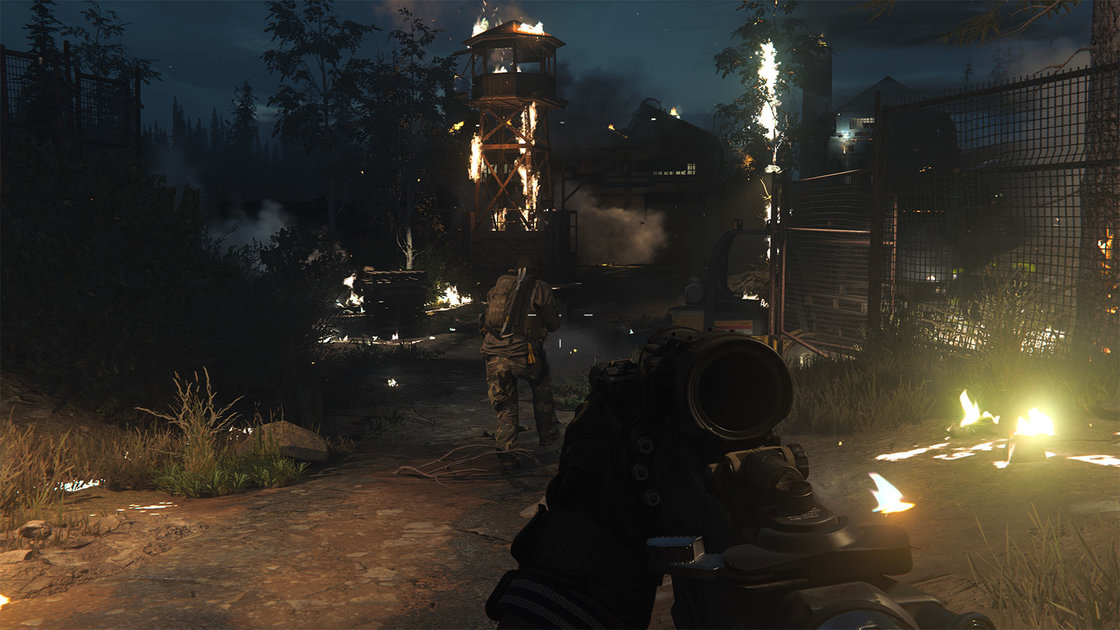
\includegraphics[width=1\textwidth]{images/cod.jpg} % first figure itself
        \caption{Widok z perspektywy pierwszej osoby z gry Call of Duty.}
        \caption*{Źródło: https://www.pocket-lint.com /games/reviews/activision/150364-call-of-duty-modern-warfare-review}
        \caption*{Data dostępu: 12.05.2020}
        \label{fig:cod}
    \end{minipage}\hfill
    \begin{minipage}{0.45\textwidth}
        \centering
        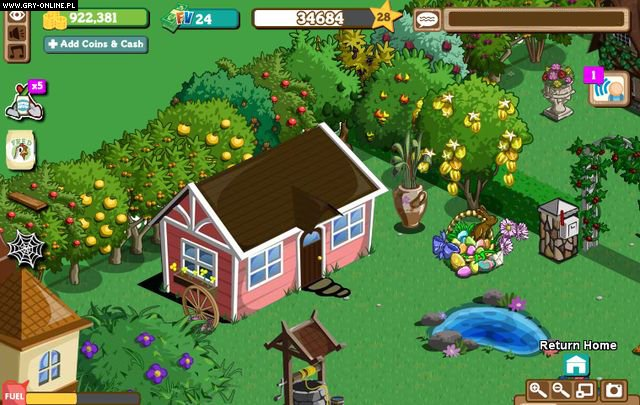
\includegraphics[width=1\textwidth]{images/farm.jpg} % second figure itself
        \caption{Widok gracza wraz z interfejsem użytkownika z gry FarmVille.}
        \caption*{Źródło: https://www.pocketgamer.com /games/023284/farmville-2-country-escape/screenshots/}
        \caption*{Data dostępu: 12.05.2020}
        \label{fig:farm}
    \end{minipage}
\end{figure}

Twórcy gier z reguły kopiują metody wywołania emocji z uznanych już wcześniej mediów - literatury i filmu. Gracze grają w gry dla doświadczenia pewnego przeżycia, a gry mają zdolność symulowania emocji w formie bliższej prawdziwemu życiu niż filmy czy książki. Mając to na uwadze, gry powinny mieć potencjał wywoływania silnych emocji, w połączeniu z konwencjonalnymi sposobami wykorzystanymi w wyżej wymienionych mediach, ale również bez ich wykorzystania. Jeśli chodzi o wywołanie emocji, potencjał gier wydaje się większy \citep{button, movesus}.

\section{Wymiary emocji}

Teorie emocji mówią, że ludzie są ewolucyjnie wyposażeni w ograniczony zestaw podstawowych emocji. Każda podstawowa emocja jest niezależna od innych w jej behawioralnych (związanych z zachowaniem), psychologicznych i fizjologicznych przejawach. Wyróżnia się sześć podstawowych emocji, a mianowicie \citep{colors}:
\begin{itemize}
  \item gniew,
  \item strach,
  \item wstręt,
  \item radość,
  \item smutek,
  \item zaskoczenie.
\end{itemize}

Większość teoretyków podziela pogląd, że emocje składają się z trzech głównych elementów: subiektywnego odczuwania, ekspresji i reakcji fizjologicznej. Jedne są motywacyjne i mają tendencję do wprowadzenia w stan motywacyjny lub tendencję do działania \citep{games}.

Istnieje możliwość określenia emocji, badając mimikę i reakcje fizjologiczne. Emocje można mierzyć również pośrednio za pomocą reakcji emocjonalnych. Badania pozwoliły na stworzenie modelu reakcji emocjonalnych.  Wymiarowa teoria emocji utrzymuje, że wszystkie emocje mogą znajdować się w dwuwymiarowej przestrzeni, jako współrzędne walencji oraz pobudzenia \citep{games}.

Jednym z często używanych modeli jest „kołowy model afektu” stworzony przez Russella w 1980 roku, który został przedstawiony na rysunku \ref{fig:spectrum}. Charakteryzuje on emocje w kategoriach dwóch wymiarów reakcji emocjonalnych, a mianowicie pobudzenia i walencji. Pobudzenie to fizjologiczny i psychologiczny stan bycia pobudzonym (aktywacja) lub brakiem pobudzenia (dezaktywacja) na bodźce. Walencja jest wewnętrznie pozytywnym (przyjemnym) lub negatywnym (nieprzyjemnym) uczuciem, które jest wywołane przez wydarzenie, przedmiot lub sytuację \citep{colors}.

\begin{figure}[h]
	\centering
	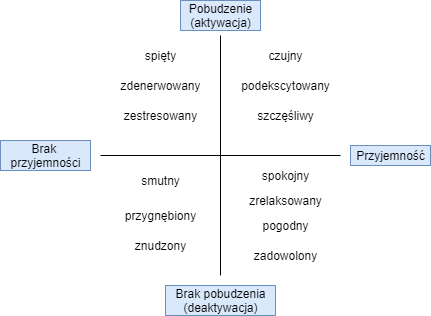
\includegraphics[width=0.85\textwidth]{images/diagram2.png}
	\caption{Kołowy model afektu stworzony przez Jamesa Russella. Oś pozioma odpowiada za walencję, a pionowa za stan pobudzenia.}
	\caption*{Źródło: opracowanie własne na podstawie \citep[s.1]{colors}.}
	\label{fig:spectrum}
\end{figure}


\section{Emocjonalne reakcje graczy}

Istnieje niewiele badań analizujących reakcje emocjonalne na gry z punktu widzenia doświadczenia użytkownika. Jednak niektóre badania dotyczyły jedynie negatywnie ocenianych emocji wywoływanych przez gry wideo, próbując rozwikłać ich potencjalne niekorzystne skutki. Badania były sprzeczne - jedne stwierdzały, że brutalne gry wideo wywołują wrogi afekt np. lęk, inne z kolei, że nie wywołują żadnego afektu. Ewentualnie niepokój może wynikać z obserwacji poziomu symbolicznej agresji, jaką samemu dokonuje się w grze. W odniesieniu do fizjologicznego komponentu emocji powszechnie wiadomo, że zadania wymagające wysiłku poznawczego lub aktywnego radzenia sobie wywołują pobudzenie emocjonalne, któremu towarzyszy m.in. przyspieszenie tętna. W badaniach nad psychofizjologiczną reaktywnością na stres, gry wideo były często wykorzystywane jako stresor. Kilka badań wykazało, że różne gry wideo wywołują znaczną reaktywność sercowo-naczyniową. Odkryto również, że dwuosobowa gra wideo na przykładzie „piłki nożnej” ma większy wpływ na tętno w porównaniu z grą wideo „trening squasha” przeciwko maszynie, co może sugerować, że sytuacja konkurencji społecznej związana z poprzednią grą powoduje zwiększone pobudzenie \citep{games}.


\section{Narzędzia wykorzystywane do wywołania emocji w grach}

\subsection{Awatar}

Awatar to byt, który wywodzi się z hinduskiej koncepcji boga wcielonego w różne istoty. Cyfrowy awatar to postać w wirtualnym świecie, która reprezentuje gracza. Bywają z góry zdefiniowane (tak jak postacie filmowe) lub istnieje możliwość  modyfikacji ich różnych cech: wyglądu, charakteru lub poziomu umiejętności \citep{glossary}.

Awatar jest często używany jako sposób na przeniesienie gracza do świata gry. Awatarów może być kilka i można ich używać na różne sposoby, ale łączy je to, że służą jako przedłużenie tożsamości gracza. Percepcja może wykroczyć poza świat realny, przenikając do wirtualnego i to samo dzieje się z tożsamością. Można to przyrównać do jazdy samochodem, kiedy podczas jazdy kierowca wyczuwa pozycje samochodu w przestrzeni, a ściślej określając do tzw. intuicyjnego ``wyczucia samochodu'' na przykład podczas parkowania - wtedy samochód staje się przedłużeniem ciała i jaźni \citep{gamefeel}.

Przedłużenie zmysłów gracza poprzez wcielenie się w postać pozwala zatracić się użytkownikowi w świecie gry. Daje to twórcom możliwość wywołanie różnych emocji u gracza, które odczuwa postać, w zależności od wydarzeń, które miały miejsce w symulowanym świecie. Zdarzenia występujące w grze np. walka postaci z lwem, może wywołać różne stany emocjonalne u różnych graczy - jedni poczują strach i wycofanie przed trudnym przeciwnikiem, inni z kolei będą pobudzeni i podekscytowani - gotowi na stoczenie walki. Tak więc mechanizm wywołania emocji w grze może być diametralnie inny od tego, który spotykamy w filmach, gdzie odczuwanie emocji jest zdeterminowane przez bierną obserwację poczynań bohaterów oraz ich przeżyć emocjonalnych. Emocje wywołane przez gry są zatem bardziej osobiste, ale trudniej je kontrolować twórcom. Składa się to na doświadczenie, będące dużo bardziej realne niż to filmowe \citep{button}.

\subsection{Interaktywność}

Interaktywność w kontekście gier, to termin, który jest używany do opisania jak gracz doświadcza historii, mechaniki i środowiska gry. Pozwala na zainteresowanie i zaangażowanie gracza. Podstawą tworzenia gier i główną cechą, która odróżnia gry od filmów jest interaktywność, co pozwala na nazwanie czynności grania aktywnym użyciem medium. W przeciwieństwie do pasywnych użyć mediów, aktywne ich użycie zmienia reakcje organizmu - zwiększa czujność poznawczą, tak więc granie w godzinach wieczornych może doprowadzić do wydłużenia czasu, który jest potrzebny na przejście z czasu czuwania do pełnego snu. Większość gier może być trudna do skończenia bez odpowiednich umiejętności i obycia ze sprzętem - tak więc gry wymagają od gracza uwagi i mocnego zaangażowania w to co się dzieje co może być dodatkowo bardzo skutecznie wykorzystane do wywołania emocji \citep{button, website:interactive}.

\subsection{Kontrola}

Kluczem do przeniesienia tożsamości gracza do świata gry jest kontrola w czasie rzeczywistym- czyli sterowanie poczynaniami awatara. Sterować można postaciami jak i bytami abstrakcyjnymi. Gry oparte na systemie turowym, lub takie, w których gracz nie wciela się w postać w pierwszej osobie, lecz sprawuje kontrolę pośrednio wydając rozkazy utrudniają identyfikację gracza z awatarem \citep{button}.

Urządzenia wejścia również przekładają się na satysfakcję gracza. Bardziej naturalne sposoby kontroli pozwalają na mocniejsze zatracenie się w grze. Użycie akcesoriów jak np. kierownica do grania w gry typu wyścigi, dostarczy graczowi dużo większych emocji niż kierowanie wirtualnym samochodem przy użyciu klawiatury \citep{button}.

Przeniesieniu tożsamości na awatar, pozwala graczowi na przeżycie tego co dzieje się na monitorze personalnie. Stąd też podczas animowanych przerywników filmowych w grach, gracz utożsamiający się z postacią przeżyje wydarzenia, które dzieją się na ekranie w sposób emocjonalny \citep{button, gamefeel}.

\subsection{Poczucie sprawczości}

Poczucie sprawczości występuje kiedy gracz bierze czynny udział w powieści i ma wpływ na jej przyszłe losy. W momentach, kiedy gracz tego doświadcza nie skupia się on na tym co aktualnie dzieje się w historii, natomiast na tym co stanie się w przyszłości, jeśli jakieś konkretne działania zostaną przez niego podjęte. Dzięki temu gracz czuje się odpowiedzialny, za to co dzieje się w fabule, nawet jeśli jego wpływ na nią jest bardzo mały. Taka zmiana pozwala na mocniejsze zaangażowanie i łatwiejsze wywołanie u niego konkretnych stanów emocjonalnych \citep{button, glossary}. 

Doświadczenie sprawczości to unikalne narzędzie wykorzystywane przez twórców gier. Poprzez dobrze zaprojektowane doświadczenie, gracz poczuje się odpowiedzialny za znacznie więcej niż w rzeczywistości, przy jednoczesnej oszczędności zasobów na zbyt szeroką i rozgałęzioną ścieżkę  \citep{button}.

\subsection{Symulowane akcje}

Symulowane akcje w kontekście gier występuje wtedy, kiedy interaktywność w grze wykracza poza korzystanie z funkcji interfejsu użytkownika. Elementy sterujące w grze mogą być zaprojektowane w sposób, który wywołuje emocje, jeśli tylko są one połączone z odpowiednią akcją. Dzieje się to najczęściej poprzez naśladowanie przez te elementy obiektów fizycznych. Jednym z przykładów symulowanej akcji może być proces przebiegu czasu. Ten wygenerowany przez świat gry wywołuje silne emocje, kiedy to na przykład pewne zadania muszą zostać rozwiązane w ograniczeniu czasowym - podobnie jak w sytuacjach generujących emocje w prawdziwym życiu. W takim przypadku gracz musi szybko zintegrować: procesy poznawcze, emocje oraz akcje w celu odniesienia sukcesu \citep{button}.

Kolejnym przykładem jest naśladowanie obiektów lub akcji występujących w grze przez kontrolery, które służą do sterowania. Niektóre są zbudowane tylko w celu imitacji danego elementu takie jak na przykład kierownice do samochodów lub drążki do latania. Pozwalają one na wywołanie silniejszych i bardziej realnych przeżyć u gracza, ale są za to mniej uniwersalne od klasycznych kontrolerów \citep{button}.

\subsection{Interaktywny dyskomfort}

Gry wideo nie zawsze muszą być zabawą i sprawiać radość. Podobnie jak inne media, mogą wywoływać różne rodzaje emocji i doświadczeń. Dyskomfort można wywołać na wiele różnych sposobów i chociaż może wydawać się to negatywnym zjawiskiem, może być odbierane pozytywnie. Zależy to od kontekstu - wiele graczy gra w gry wyłącznie dla negatywnie nacechowanych emocji np. strachu w grach typu horror \citep{button}.

Na podstawie badań J.A. Bopp negatywne emocje wywołane w grach mogą prowadzić do pozytywnych doświadczeń. Gracze oceniają gry nie tylko, ze względu na wywoływanie konkretnie nacechowanych emocji, ale także ze względu na fakt, że gra wywołuje silne reakcje emocjonalne, np. strach \citep{negativeemotions}.

% Na podstawie badań J.A. Bopp negatywne emocje wywołane w grach mogą prowadzić do pozytywnych doświadczeń. Gracze oceniają gry nie tylko, ze względu na wywoływanie konkretnie nacechowanych emocji, ale także, ze względu na wywołanie silnych reakcji emocjonalnych. 

% także ze względu na fakt, że gra wywołuje silne reakcje emocjonalne, np. strach \citep{negativeemotions}.


\subsection{Wyzwanie}

Wyzwanie to integralna część większości gier komputerowych występująca w różnorakiej formie. Głównymi czynnikami decydującymi o wyzwaniu są umiejętności gracza: czas reakcji, umiejętność prowadzenia wielu zadań na raz (tzw. multitasking) czy wysoki poziom opanowania kontrolera. Założenie określonego poziomu umiejętności dla wszystkich potencjalnych graczy jest niemożliwe, ale jeśli wyzwanie jest na odpowiednim poziomie dla konkretnego gracza, może on wejść w stan przepływu (ang. flow). Określa to tzw. Teoria Przepływu, którą Swink opisuje następująco: 
``Teoria przepływu mówi, że kiedy wyzwanie, które podejmujesz jest bardzo bliskie twojemu obecnemu poziomowi umiejętności, wejdziesz w stan ``flow'', który charakteryzuje się utratą samoświadomości,  zniekształconym postrzeganiem czasu i mnóstwem przyjemnych wrażeń. Jeśli twoje umiejętności są znacznie większe niż wyzwanie jakie daje Ci dana czynność, będziesz się nudzić, a jeśli twoje umiejętności są znacznie poniżej poziomu przewidzianego wyzwania będziesz sfrustrowany'' \citep[s.~23]{gamefeel}. Wyzwanie często jest używane aby wprowadzić gracza w stan ``flow'', co również  również potęguje jego emocje wynikające z rozgrywki \citep{button, gamefeel}.

\subsection{Doświadczenie społeczne - rozgrywka wieloosobowa}

W grach wieloosobowych działania każdej postaci z osobna łączą się tworząc jedno, społeczne doświadczenie pomiędzy graczami. Pomimo tego, że gracz nie znajduje się w realnym, lecz w ``wirtualnym świecie'', wykorzystuje się narzędzia, które pozwalają zaangażować się w społeczne odgrywanie ról przez awatary. Hybrydowy charakter tych doświadczeń, które są zarazem realne i wirtualne, pozwala na większe zaangażowanie graczy, którzy wcielają się w wykreowane postacie. W efekcie to projektanci gier kształtują środowisko społeczne oraz to w jaki sposób budowane są więzi społeczne między wieloma graczami, poprzez definicje sposobu interakcji między nimi \citep{movesus}.

\subsection{Zaangażowanie ciała}

Ciało znacząco kształtuje doświadczenie emocjonalne - tak samo w rozgrywce jak i w prawdziwym życiu. Od pojawienia się kontrolerów i urządzeń opartych na ruchu, twórcy gier mogą pozwolić na wykorzystanie ciała graczy jako medium do kształtowania emocji, bądź więzi społecznych. Projektanci gier wprowadzają coraz to bardziej innowacyjne rozwiązania, które pozwalają na wywołanie szerokiej palety emocji poprzez łączenie technologii, świata rzeczywistego i wyobraźni. Dzieje się tak na przykład poprzez zastosowanie strategii wymagających od graczy opanowania zmęczenia i bólu lub ułożenia ciała w sposób, który wywołuje fizyczną bliskość lub wymaga wyjścia ze strefy komfortu. Zamiast unieruchamiać ciało lub izolować graczy od innych ludzi, gry w przyszłości mogą obejmować i wzmacniać rolę ciała i jego fizycznej aktywności w grze. Połączenie fizyczne i emocjonalne może wspierać ludzi w dążeniu do osiągnięcia określonych efektów jak na przykład wytrenowanie wymarzonej sylwetki \citep{movesus}.
\chapter{Wywoływanie emocji w grach VR i grach wideo}
\label{chap:czwarty}

\section{Cel badania, technika badawcza, przebieg badania}

Celem badania jest zdobycie wiedzy czy i jakie emocje w grach są pożądane z perspektywy użytkownika, biorąc pod uwagę formę rozgrywki, zbadanie  preferencji i cech grupy badawczej pod względem konkretnej platformy i gatunku gier oraz zbadanie predyspozycji konkretnych mediów do wywołania określonych emocji u użytkownika. Poszukiwano odpowiedzi na następujące pytania badawcze:

\begin{enumerate}
   \item Jaka jest charakterystyka graczy preferujących gry wideo, a jaka preferujących gry VR?
   \item Czym charakteryzuje się rozgrywka w gry typu VR, a czym w gry wideo?
   \item Czy emocje w grach są pożądane z perspektywy graczy oraz jaki jest związek pomiędzy platformą a wywołanymi emocjami?
\end{enumerate}

W celu zapoznania się z preferencjami użytkowników w badaniu wykorzystano technikę, jaką jest badanie ankietowe, które składało się z pytań zamkniętych oraz pytań otwartych (zob. Dodatek, str.\pageref{chap:dodatek}). Pytania otwarte nie były obowiązkowe i miały na celu określenie przez respondentów wad oraz zalet obu form gier komputerowych. Ankieta składała się z 20 pytań, które można podzielić na 3 grupy, biorąc pod uwagę cel pytań:
\begin{itemize}
  \item zbadanie cech grupy badawczej,
  \item zbadanie preferencji grupy badawczej,
  \item zbadanie predyspozycji platformy do wywołania określonych emocji.
\end{itemize}

Grupą docelową badania były osoby korzystające z gier VR i gier wideo. Badanie ankietowe zostało przeprowadzone w wersji elektronicznej przy użyciu formularza ``Google Forms''. Ankieta została rozesłana do osób związanych ze środowiskiem gier wideo, a także udostępniona w prywatnych grupach miłośników gier VR przy użyciu mediów społecznościowych. Dane były zbierane przez okres 3 tygodni, w dniach:  6.07.2020 - 26.07.2020. Autorowi pracy zależało na różnorodności osób badanych, głównie pod względem wieku oraz preferencji związanych z daną platformą.

\section{Charakterystyka grupy badawczej}

Ankieta została wypełniona przez 107 osób, z czego 7 nie brano pod uwagę w dalszej części badania ze względu na brak doświadczenia z grami wideo i grami VR. Na pytania otwarte opowiedziało 32 osoby, co zostało dokładniej opisane w jednym z kolejnych podrozdziałów. Większość respondentów stanowili mężczyźni (72). Tylko 28 kobiet wypełniło ankietę.

Podział względem wieku ilustruje tabela \ref{tbl:twiek}. Najwięcej badanych to osoby w wieku 26 - 40 lat, a najmniejszą liczbę stanowią najmłodsi, czyli osoby poniżej 16 roku życia.

\begin{table}[htb]
  \centering
  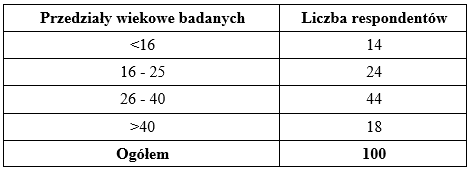
\includegraphics[width=0.75\textwidth]{images/twiek.PNG}
  \caption{Wiek osób biorących udział w badaniu.}
  \caption*{Źródło: opracowanie własne.}
  \label{tbl:twiek}
\end{table}

W tabeli \ref{tbl:twyksztalcenie} zilustrowany jest podział respondentów względem wykształcenia. Najwięcej osób, które udzieliły odpowiedzi posiadają wykształcenie wyższe (54\%). Osoby z wykształceniem średnim i podstawowym stanowią kolejno 26\% oraz 9\%. Pozostałe wykształcenie, opisane jako inne posiadało 11\% badanych.

\clearpage

\begin{table}[htb]
  \centering
  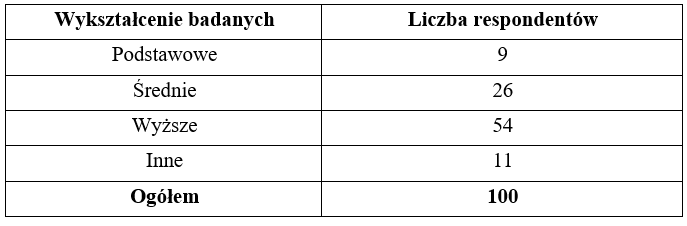
\includegraphics[width=0.85\textwidth]{images/twyksztalcenie.PNG}
  \caption{Wykształcenie osób biorących udział w badaniu.}
  \caption*{Źródło: opracowanie własne.}
  \label{tbl:twyksztalcenie}
\end{table}

Na tym etapie zbadano liczbę osób, które miały doświadczenie z grami VR jak i grami wideo. Odrzuceni zostali respondenci, którzy nie mieli styczności z żadną z platform. Większość z osób, bo aż 93\% korzystało z obu platform, osób korzystających tylko z gier VR było 2\%, a tylko gier wideo 5\%, co ukazuje rysunek \ref{figure:dplatformy}.

\begin{figure}[htb]
  \centering
  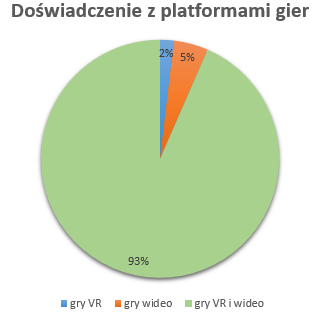
\includegraphics[width=0.6\textwidth]{images/dplatformy.PNG}
  \caption{Doświadczenie z platformami gier osób biorących udział w badaniu.}
  \caption*{Źródło: opracowanie własne.}
  \label{figure:dplatformy}
\end{figure}

\clearpage

\section{Wyniki}

\subsection{Wiek gracza a ulubiona platforma}

Gry wideo jako ulubione medium wybrało 49\% ankietowanych, natomiast gry VR 51\%. Podział ten jednak nie jest tak równomierny w odniesieniu to wieku graczy, co ilustruje rysunek \ref{figure:dwiek}.

\begin{figure}[htb]
  \centering
  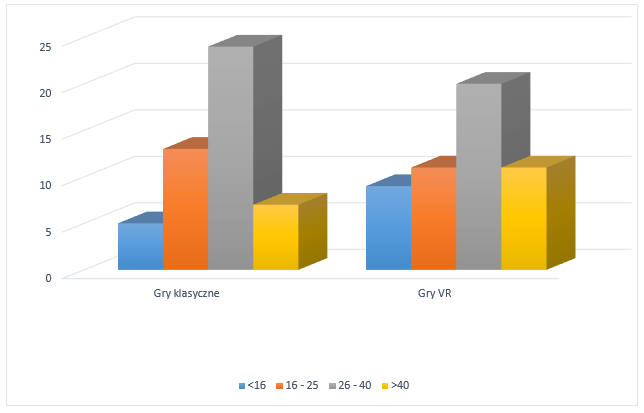
\includegraphics[width=0.9\textwidth]{images/dwiek.PNG}
  \caption{Podział wiekowy użytkowników względem ulubionej platformy.}
  \caption*{Źródło: opracowanie własne.}
  \label{figure:dwiek}
\end{figure}

Z rysunku \ref{figure:dwiek}  wynika, że najmłodsza jak i najstarsza grupa (poniżej 16 oraz powyżej 40 roku życia) badanych preferuje rozgrywkę w trybie VR, natomiast osoby z przedziału wiekowego 16-40 wybierają częściej rozgrywkę w postaci gier wideo. 

\subsection{Czas jednej rozgrywki}

Dane ukazane w tabeli \ref{tbl:tczas} przedstawiają, że czas poświęcony na jedną sesję grania w gry VR, a gry wideo znacząco się różni. W przypadku VR 38\% osób poświęca na grę mniej niż jedną godzinę, a aż 49\% 1 - 2 godzin. Odpowiedź 2 - 5 godzin zaznaczyło 13\%. Żaden z korespondentów nie odpowiedział, że poświęca średnio podczas jednej sesji więcej niż 5 godzin.

Natomiast w przypadku grania w gry wideo, czas poświęcony na jedną sesję, która wynosi mniej niż godzinę to 15\%, a 1 - 2 godzin 33\%. Największy odsetek graczy poświęca na jedną sesję 41\%, a 10\% odpowiadających gra jednorazowo powyżej 5 godzin. 

\clearpage

\begin{table}[htb]
  \centering
  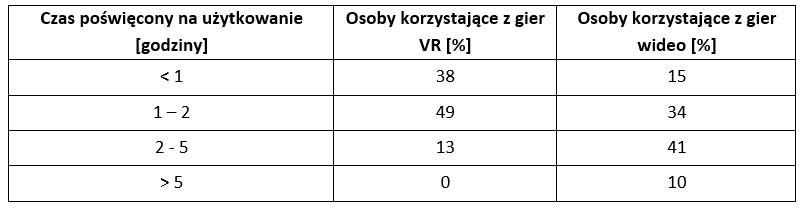
\includegraphics[width=0.8\textwidth]{images/tczas.PNG}
  \caption{Czas poświęcony na użytkowanie przez graczy danej platformy podczas jednej sesji.}
  \caption*{Źródło: opracowanie własne.}
  \label{tbl:tczas}
\end{table}

\subsection{Częstotliwość grania}

Podobna różnorodność jak w przypadku czasu jednej rozgrywki występuje w porównaniu częstotliwości grania w gry VR i gry wideo. Osoby grające rzadziej niż raz w miesiącu stanowią 30\% w przypadku korzystania z technologii VR, oraz 9\% w przypadku korzystania z gier wideo. Wybór przedziału w postaci 1 - 4 razy w miesiącu dokonało kolejno: dla VR 55\%, co było najczęściej wybieraną odpowiedzią, a dla gier wideo 34\%. Kilka razy w tygodniu natomiast z VR korzysta 14\% graczy, a aż 47\% z gier wideo. Najmniej osób odpowiedziało, że gra codziennie w VR (1\%) oraz w gry wideo (11\%).

\begin{table}[htb]
  \centering
  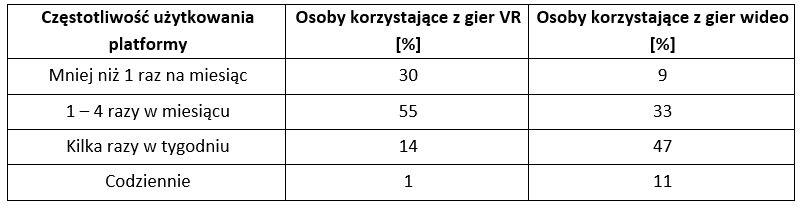
\includegraphics[width=0.9\textwidth]{images/tczestotliwosc.PNG}
  \caption{Częstotliwość użytkowania danej platformy przez graczy.}
  \caption*{Źródło: opracowanie własne.}
  \label{tbl:tczestotliwosc}
\end{table}

\subsection{Immersja a zmęczenie}

Pomimo tego, że respondenci podzielili się na dwie równe grupy jeśli chodzi o preferencje platformy (VR 51\% oraz gry wideo 49\%) to w pytaniach dotyczących wywołania zmęczenia przez grę oraz zdolności gry do pochłonięcia uwagi gracza i wywołania silnych emocji, większość była zgodna. Wyniki tego zestawienia przedstawia tabela \ref{tbl:tzmeczenie}.

\begin{table}[htb]
  \centering
  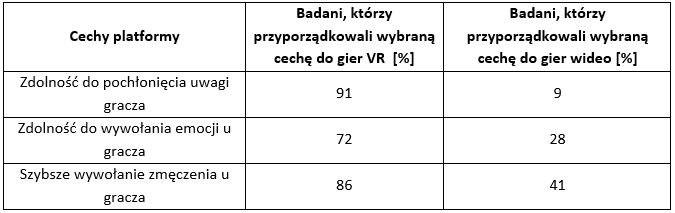
\includegraphics[width=0.9\textwidth]{images/tzmeczenie.PNG}
  \caption{Przyporządkowanie określonych cech do jednej z platform przez ankietowanych.}
  \caption*{Źródło: opracowanie własne.}
  \label{tbl:tzmeczenie}
\end{table}

\subsection{Zdolność platformy do wywołania specyficznych emocji a poziom jej pożądania przez graczy}

Tabela \ref{tbl:tpredyspozycje} wyłania najbardziej i najmniej pożądaną emocję wśród graczy, a także ukazuje predyspozycje gier VR oraz gier wideo do wywołania konkretnych emocji.

\begin{table}[htb]
  \centering
  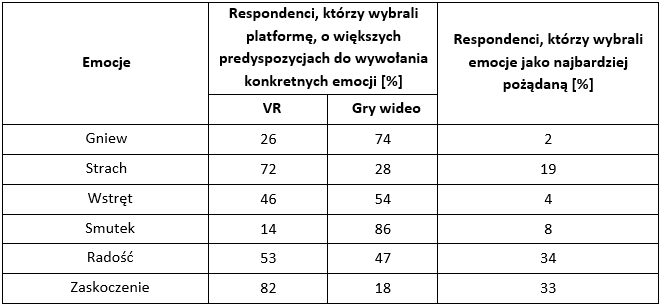
\includegraphics[width=0.8\textwidth]{images/tpredyspozycje.PNG}
  \caption{Emocje i predyspozycje danej platformy do łatwości jej wywołania oraz ważność konkretnej emocji dla graczy.}
  \caption*{Źródło: opracowanie własne.}
  \label{tbl:tpredyspozycje}
\end{table}

Najbardziej pożądaną emocją wśród respondentów okazuje się radość, którą wybrało 34\%. Kolejno były to: zaskoczenie(33\%), strach(19\%), smutek(8\%), wstręt(4\%), gniew(2\%).


Ankietowani wybierali platformę, która ma według nich większe predyspozycje do wywołania konkretnych emocji. Z ankiety wynika, że przy użyciu VR łatwiej wywołać takie emocje jak: zaskoczenie(82\%), strach(72\%) oraz radość(53\%), jednak to gry wideo mają większe predyspozycje do wywołania takich emocji jak: gniew(74\%), wstręt(54\%), smutek(86\%). 

\subsection{Ulubione gatunki gier i ich elementy}

Ulubione gatunki uczestników ankiety przedstawia rysunek \ref{fig:dgatunek}. Większość respondentów za ulubiony gatunek gier wybrało gry zręcznościowe (31\%). Później kolejno: gry sportowe i symulacyjne (29\%), gry przygodowe i fabularne (23\%). Najmniej respondentów uważa za swój ulubiony gatunek gry strategiczne (17\%).

\begin{figure}[htb]
  \centering
  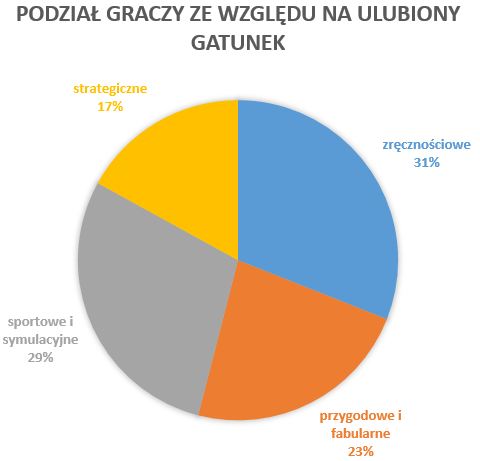
\includegraphics[width=0.8\textwidth]{images/dgatunek.PNG}
  \caption{Ulubione gatunki gier wybrane przez graczy.}
  \caption*{Źródło: opracowanie własne.}
  \label{fig:dgatunek}
\end{figure}

\clearpage

Najbardziej znaczącym elementem rozgrywki dla respondentów okazało się ``wyzwanie, rywalizacja i osiągnięcie sukcesu'' - odpowiedziało tak 43\% ankietowanych, najmniej znaczącym elementem (12\%) zostało ``zaangażowanie ciała w rozgrywkę''. ``doświadczenie społeczne'' oraz ``fabuła, historia, wpływ na jej losy'' są najważniejszym elementem dla podobnej liczby graczy bo kolejno: 22\% i 23\%, co przedstawia tabela \ref{tbl:telementy}.

\begin{table}[htb]
  \centering
  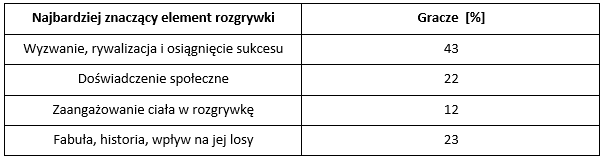
\includegraphics[width=0.8\textwidth]{images/telementy.PNG}
  \caption{Najbardziej znaczące elementy rozgrywki dla graczy.}
  \caption*{Źródło: opracowanie własne.}
  \label{tbl:telementy}
\end{table}

\subsection{Wady i zalety obu platform}

Respondenci w pytaniach otwartych udzielili odpowiedzi na pytanie jakie są wady i zalety obu platform. Na podstawie najczęściej występujących odpowiedzi stworzona została tabela  \ref{tbl:twadyzalety}.

\begin{table}[htb]
  \centering
  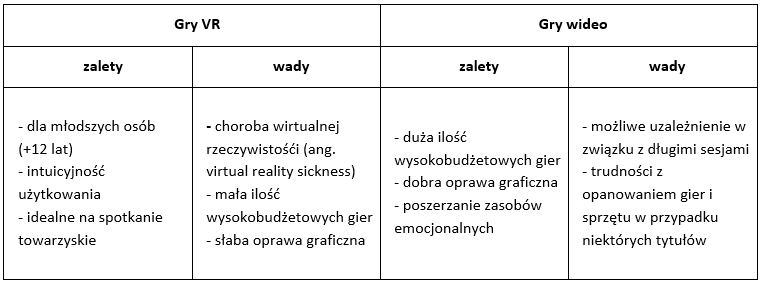
\includegraphics[width=1\textwidth]{images/twadyzalety.PNG}
  \caption{Najczęściej wymieniane wady i zalety gier VR i gier wideo przez respondentów.}
  \caption*{Źródło: opracowanie własne.}
  \label{tbl:twadyzalety}
\end{table}

   

% WNIOSKI !!!!!!!!!!!!!!!!!!!!!!!!!!!!!!!!!
    
    
\section{Wnioski}

\subsection{Preferencje graczy}

Analizując dane na temat wieku oraz preferencji co do ulubionej platformy, zauważalny jest znaczny podział na dwie grupy. Osoby najmłodsze jak i najstarsze preferują rozgrywkę w formie VR, natomiast osoby w wieku 16-40 wybierają gry wideo. Dane z ankiety pochodzą z roku 2020, więc osoby te urodziły się w latach 1980-2004. Spora część osób będących w tym przedziale swoją młodość spędzała w latach, kiedy dużą popularnością cieszyły się gry arcade, gry komputerowe oraz konsolowe, czyli te występujące po tzw. złotej erze gier arcade - lata 80,90 XX wieku oraz na początku XXI wieku.  Można wywnioskować, że osoby te miały styczność z grami w latach młodości, co pozwoliło im na obycie się z różnego typu sprzętem i wyrobiło pewne umiejętności, które przydają się w erze dzisiejszych gier wideo. Kolejną kwestią może być przyzwyczajenie użytkowników do tego typu gier. Osoby młode, czyli te poniżej 16 lat oraz osoby powyżej 40 lat mogły nie mieć okazji aby zainteresować się grami wideo. Można zauważyć, że te osoby często wybierają rozrywkę w trybie VR lub tą, dostarczaną przez urządzenia mobilne - głównie telefony typu smartfon. Potwierdzają to także odpowiedzi w pytaniach otwartych, gdzie jedną z częściej wymienianych zalet VR jest intuicyjność. Próg wejścia dla młodych graczy oraz starszych osób jeśli chodzi o gry wideo nie jest tak niski jak w przypadku gier VR.

Osoby korzystające z obu platform najczęściej wybierają gry zręcznościowe, sportowe oraz symulacyjne, a większość ankietowanych wybrało ``Wyzwanie, rywalizację i osiągnięcie sukcesu'' jako najbardziej znaczący element rozgrywki. Dowodzi to, że osoby korzystające zarówno z VR jak i gier wideo mają podobne preferencje co do gatunku gier, jak i cenią w grach podobne elementy rozgrywki. Ma to związek z tym, że gry VR polegają najczęściej na rywalizacji poprzez proste czynności, lecz bez skomplikowanej fabuły. Na podstawie danych z tabeli \ref{tbl:twadyzalety} można stwierdzić, że gry VR najczęściej wybierane są ze względu na intuicyjność, prostotę oraz formę zabawy, przeciwstawnie do gier wideo, gdzie gracze głównie oczekują rozbudowanej rozgrywki z dobrą oprawą graficzną. Można wysnuć wniosek, że preferencje graczy znacznie się różnią - część z nich zależy od konkretnych cech użytkownika, inne natomiast to kwestia zainteresowań lub upodobań.


\subsection{Charakter rozgrywki}

VR charakteryzuje się dużą zdolnością do wywołania emocji oraz bardzo łatwo pochłania uwagę gracza. Analizując dane wykryto zależność między kilkoma czynnikami:
\begin{itemize}
  \item zdolnością VR do pochłonięcia uwagi gracza,
  \item zdolnością VR do wywołania emocji,
  \item częstotliwością grania,
  \item czasem grania.
\end{itemize}

Spoglądając na dane, można stwierdzić, że osoby korzystające z VR najczęściej poświęcają na grę maksymalnie 2 godziny podczas jednej sesji, która odbywa się od 1 do 4 razy w miesiącu. Inny charakter ma korzystanie z gier wideo - kiedy to pojedyncza sesja trwa najczęściej od 2 do 5 godzin i jest odbywana kilka razy w tygodniu. Analizując te dane można zauważyć pewną zależność - zdolność gier do dużej immersji prowadzi do wywołania silnych emocji, co z kolei negatywnie skutkuje zmęczeniem fizycznym oraz psychicznym po krótkiej rozgrywce, dlatego osoby sięgają po gry VR rzadziej jak i na krótszy czas. Gry wideo z kolei są mniej męczące, bardziej komfortowe i pozwalają na częstszą i dłuższą rozgrywkę. Gry wideo z reguły dostarczają mniej intensywnych przeżyć niż gry VR, ale pozwalają na większy relaks i odpoczynek. 

\subsection{Predyspozycje platform do wywołania specyficznych emocji u użytkownika}

%OLD  

% Zarówno gry VR jak i gry wideo są dobrym sposobem na wywołanie emocji u swoich użytkowników. Większość z ankietowanych odpowiedziało, że zdolność gier do wywołania określonych stanów emocjonalnych jest dla nich bardzo ważna. VR dzięki swoim cechom ma dużą zdolność do wywołania emocji podczas rozgrywek lecz ze względu na początkowe stadium rozwoju tej technologii w porównaniu do gier wideo nie ma ona tak dużo zwolenników. Z ankiety wynika, że to VR ma większe predyspozycje do wywołania najbardziej pożądanych emocji przez graczy (radość, zaskoczenie, strach) lecz nie jest tak popularną formą rozrywki jak gry wideo. Aktualne liczbę graczy ogółem na świecie szacuje się na ponad 2.5 miliarda, z czego gracze VR to tylko 171 milionów\citep{website:gameindustry, website:vrstats}. Liczba ta ciągle rośnie, a to za sprawą wciąż rozwijającej się technologii VR. Największą zmorą VR jest brak "pełnoprawnych" gier, lecz i to ulega zmianie. Wydanie jednej, dobrze przyjętej przez graczy produkcji może znacząco zmienić liczbę aktywnych graczy. Przykładem może być wydanie gry "Half-Life: Alyx", kiedy  w ciągu jednego miesiąca odnotowano przyrost 1 miliona nowych użytkowników VR\citep{website:alyx}.

%  NEW

% Technologia VR pozwala na wywołanie silnych i intensywnych emocji u swoich
% użytkowników, lecz niesie to za sobą także negatywne skutki, stad wiele osób wybiera
% klasyczne gry wideo. Zestawiając obie formy użytkowania gier (tj. wideo i VR) oraz biorąc
% pod uwagę emocjonalność gracza możemy wyodrębnić wiele zalet i wad, które wpływają na
% wywoływanie danego afektu u użytkownika. Wybór platformy zależy w głównej mierze od
% tego, jakiego rodzaju rozrywki oczekuje użytkownik. Intensywność wywołanych emocji, ich
% nacechowanie oraz sposób rozgrywki znacząco się różni w przypadku obu platform stąd
% porównywanie, która z nich jest lepsza wydaje się być bezcelowe. Gry VR często występują
% w nieskomplikowanych formach, aniżeli jako pełnoprawny produkt konsumencki. Jednym z
% wyjątków jest wymieniony wielokrotnie w pracy ‘Half Life Alyx’, który można nazwać
% faktyczną pełnoprawną wersją gry VR. Jak zostało opisane w tekście, każda forma wpływa na
% inny rodzaj emocji. Tak samo postrzegają to ankietowani, wg których znaczną przewagę nad
% wywoływaniem m.in. zaskoczenia ma technologia VR.

%  NEW NEW

Zarówno gry VR jak i gry wideo są dobrym sposobem na wywołanie emocji u swoich użytkowników. Większość z ankietowanych odpowiedziało, że zdolność gier do wywołania określonych stanów emocjonalnych jest dla nich bardzo ważna. Najbardziej pożądanymi emocjami są kolejno: radość, zaskoczenie i strach. Najmniej natomiast: gniew wstręt oraz smutek. 

VR dzięki swoim cechom ma dużą zdolność do wywołania emocji podczas rozgrywek lecz ze względu na początkowe stadium rozwoju tej technologii w porównaniu do gier wideo nie ma ona tak dużo zwolenników. Technologia VR pozwala na wywołanie silnych i intensywnych emocji u swoich
użytkowników, lecz niesie to za sobą także negatywne skutki (zmęczenie psychiczne i fizyczne oraz symptomy choroby wirtualnej rzeczywistości - podobne do choroby lokomocyjnej), stąd wiele osób wybiera klasyczne gry wideo.

Z ankiety wynika, że to VR ma większe predyspozycje do wywołania najbardziej pożądanych emocji przez graczy (radość, zaskoczenie, strach) lecz nie jest tak popularną formą rozrywki jak gry wideo. Zauważyć więc można związek między platformą a rodzajem emocji które wywołuje. VR znacząco lepiej radzi sobie z wywołaniem zaskoczenia oraz strachu w porównaniu do gier wideo, które z kolei lepiej radzą sobie z wywołaniem smutku u graczy. Predyspozycje platform do wywołania radości i wstrętu są bardzo zbliżone, natomiast większość badanych wybrało gry wideo jako platformę mającą większą zdolność do wywołania gniewu. Analizując dane wywnioskować można, że chociaż nie wszystkie emocje są nacechowane pozytywnie, są one pożądane przez graczy. Tymi, które są najważniejsze dla graczy to kolejno: radość, zaskoczenie i strach, a te najmniej pożądane to gniew wstręt oraz smutek. Na podstawie analizy można wywnioskować, że wywołanie emocji przez gry jest pożądane z perspektywy gracza oraz można stwierdzić, że każda z platform operuje specyficznymi zdolnościami do wywołania określonych emocji. 


% % STARE !!!!!!!!!!!!!!!!!!!!!!

% \subsection{Cechy gracza}

% Analizując dane na temat wieku oraz preferencji co do ulubionej platformy, zauważalny jest znaczny podział na dwie grupy. Osoby najmłodsze jak i najstarsze preferują rozgrywkę w formie VR, natomiast osoby w wieku 16-40 wybierają gry wideo. Dane z ankiety pochodzą z roku 2020, więc osoby te urodziły się w latach 1980-2004. Spora część osób będących w tym przedziale swoją młodość spędzała w latach, kiedy dużą popularnością cieszyły się gry arcade, gry komputerowe oraz konsolowe, czyli te występujące po tzw. złotej erze gier arcade - lata 80,90 XX wieku oraz 00 XXI wieku.  Można wywnioskować, że osoby te miały styczność z grami w latach młodości, co pozwoliło im na obycie się z różnego typu sprzętem i wyrobiło pewne umiejętności, które przydają się w erze dzisiejszych gier wideo. Kolejną kwestią może być przyzwyczajenie użytkowników do tego typu gier. Osoby młode, czyli te poniżej 16 lat oraz osoby powyżej 40 lat mogły nie mieć okazji aby zainteresować się grami wideo. Można zauważyć, że te osoby często wybierają rozrywkę w trybie VR lub tą, dostarczaną przez urządzenia mobilne - głównie telefony typu smartfon. Potwierdzają to także odpowiedzi w pytaniach otwartych, gdzie jedną z częściej wymienianych zalet VR jest intuicyjność. Próg wejścia dla młodych graczy oraz starszych osób jeśli chodzi o gry wideo nie jest tak niski jak w przypadku gier VR.


% \subsection{Immersja}

% VR charakteryzuje się dużą zdolnością do wywołania emocji oraz bardzo łatwo pochłania uwagę gracza. Analizując dane wykryto zależność między kilkoma czynikami:

% \begin{itemize}
%   \item zdolnością VR do wywołania emocji,
%   \item częstotliwością grania,
%   \item czasem grania.
% \end{itemize}

% Spoglądając na dane, można stwierdzić, że osoby korzystające z VR najczęściej poświęcają na grę maksymalnie 2 godziny podczas jednej sesji, która odbywa się od 1 do 4 razy w miesiącu. Inny charakter ma korzystanie z gier wideo - kiedy to pojedyncza sesja trwa najczęściej od 2 do 5 godzin, i jest odbywana kilka razy w tygodniu. Analizując te dane można zauważyć pewną zależność - zdolność gier do dużej immersji prowadzi do wywołania silnych emocji, co z kolei negatywnie skutkuje zmeczęniem fizycznym oraz psychicznym po krótkiej rozgrywce dlatego osoby sięgają po gry VR rzadziej jak i na krótszy czas. Gry wideo z kolei są mniej męczące, bardziej komfortowe i pozwalają na częstszą i dłuższą rozgrywkę. Gry wideo z reguły dostarczają mniej intensywnych przeżyć niż gry VR ale pozwala to na większy relaks i odpoczynek. 


% \subsection{Emocje jako czynnik sukcesu}

% Zarówno gry VR jak i gry wideo są dobrym sposobem na wywołanie emocji u swoich użytkowników.VR dzięki swoim cechom ma dużą zdolność do wywołania emocji podczas rozgrywek lecz ze względu na początkowe stadium rozwoju tej technologii w porównaniu do gier wideo nie ma ona tak dużo zwolenników. Z ankiety wynika, że to VR ma większe predyspozycje do wywołania najbardziej pożądanych emocji przez graczy (z reguły tych pozytywnych) lecz nie jest tak popularną formą rozrywki jak gry wideo. Większość z ankietowanych odpowiedziało, że zdolność gier do wywołania określonych stanów emocjonalnych jest dla nich ważna lub najważniejsza.

% Aktualne liczbę graczy ogółem na świecie szacuje się na ponad 2.5 miliarda, z czego gracze VR to tylko 171 milionów\citep{website:gameindustry, website:vrstats}. Liczba ta ciągle rośnie, a to za sprawą wciąż rozwijającej się technologii VR. Największą zmorą VR jest brak "pełnoprawnych" gier, lecz i to ulega zmianie. Wydanie jednej, dobrze przyjętej przez graczy produkcji może znacząco zmienić liczbę aktywnych graczy. Przykładem może być wydanie gry "Half-Life: Alyx", kiedy  w ciągu jednego miesiąca odnotowano przyrost 1 miliona nowych użytkowników VR\citep{website:alyx}.

% \subsection{Preferencje użytkownika a wybór platformy}

% Granie w gry VR znacząco rózni się od klasycznej rozgrywki. Na podstawie najczęściej występujących odpowiedzi badanych na temat wad i zalet obu platform stworzona została tabela zaprezentowana poniżej.

% \begin{table}[htb]
%   \centering
%   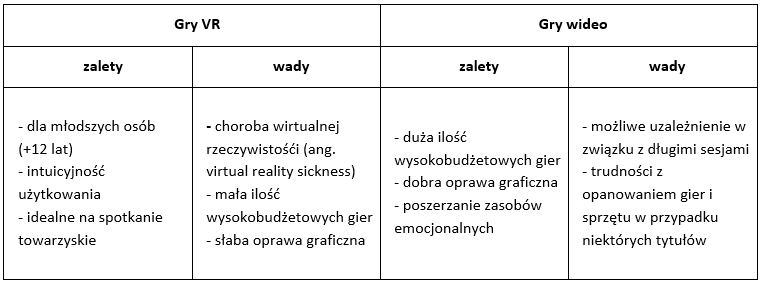
\includegraphics[width=0.8\textwidth]{images/twadyzalety.PNG}
%   \caption{Najczęściej wymieniane wady i zalety przez ankietowanych}
%   \caption*{Źródło: opracowanie własne}
%   \label{tbl:twadyzalety}
% \end{table}

% % Wybór platformy i gatunku gier zależy w głównej mierze od tego, jakiego rodzaju rozrywki oczekuje użytkownik. Intensywność wywołanych emocji, ich nacechowanie oraz sposób rozgrywki znacząco się różni w przypadku obu platform stąd porównywanie, która z nich jest lepsza wydaje się być bezcelowym. Gry wideo mają inny charakter niż gry VR, które z kolei po pewnym czasie stają się męczące i monotonne - polegają najczęsciej na prostych czynnościach, bez skompliokwanaje fabuły. Rynek VR wciąż ewoluuje i producenci gier coraz częściej będą tworzyć coraz bardziej zaawansowane dzieła, czego przykładem może być wcześniej wymieniony "Half-Life: Alyx".

\chapter*{Zakończenie}
\label{chap:zakonczenie}
\addcontentsline{toc}{chapter}{Zakończenie}


Celem pracy było opisanie czytelnikowi czym jest technologia VR,
omówienie procesu powstania emocji oraz narzędzi wykorzystywanych do ich wywołania w
grach oraz zbadanie, jakimi zdolnościami do wywołania konkretnych emocji cechują się gry VR oraz gry wideo.
    
W pierwszym rozdziale pracy zdefiniowano technologię wirtualnej rzeczywistości jako połączenie sprzętu i oprogramowania, które tworzy całkowicie nowe, cyfrowe symulacje. VR składa się z trzech głównych części jakimi są:  immersja, wyobraźnia, interakcja. W tym rozdziale została także opisana historia VR: od początków sięgających ściennych malowideł po lata współczesne, skupiające się głównie na rozrywce VR, ale także zostały podane prognozy na przyszłość mówiące o jej nowych zastosowaniach.

W kolejnym rozdziale przybliżono pojęcie emocji jako stanu umysłu, któremu towarzyszą zmiany somatyczne, akty ekspresji i działania. Dokonano  klasyfikacji emocji na funkcjonalne jak i niefunkcjonalne oraz omówiono proces powstania emocji dzieląc go na 4 składowe jakimi są: 
``ocena poznawcza'', ``wartościowanie kontekstowe'', ``gotowość do działania'' i ``zmiany psychologiczne, ekspresja, działanie''.

Trzeci rozdział poświęcony został na ukazanie związku emocji z grami. W tym celu przywołano 6 podstawowych emocji jakimi są: gniew, strach, wstręt, radość, smutek oraz zaskoczenie. Zdefiniowano grę jako aktywne medium, które jest rozróżnialne od pasywnych (np. filmów) dzięki swojej głównej właściwości jaką jest interaktywność. Wymieniono charakteryzujące gry atrybuty, które pozwalają na wywołanie emocji: użycie awatara, interaktywność, kontrolę, poczucie sprawczości, symulowane akcje, interaktywny dyskomfort, wyzwanie, doświadczenie społeczne, zaangażowanie ciała.

W ostatnim rozdziale zaprezentowano i przedyskutowano wyniki badań. Przeprowadzone badania pokazały, że preferencje graczy w stosunku do ulubionej platformy znacznie się różnią w zależności od wieku - najmłodsi i najstarsi gracze preferują rozrywkę w trybie VR, natomiast osoby w wieku od 16 do 40 lat wybierają rozrywkę w formie gier wideo. Gracze wybierają najczęściej gry zręcznościowe, sportowe oraz symulacyjne, a ich ulubioną częścią rozgrywki jest najczęściej element wyzwania, rywalizacji i osiągnięcia sukcesu. Rozgrywka graczy różni się znacząco w zależności od wybranej platformy. Osoby korzystające z gier VR odbywają krótkie sesje o małej częstotliwości z powodu negatywnych skutków, jakie powoduje częste i długie korzystanie z gogli wirtualnej rzeczywistości, natomiast osoby korzystające z gier wideo grają częściej i dłużej ze względu na bardziej relaksujący charakter rozgrywek. Pomimo że obie platformy mają dobre predyspozycje do wywołania emocji wśród graczy, to dzięki większej zdolności do pochłonięcia uwagi gracza, lepiej radzi sobie z tym technologia VR. Zauważalny jest także związek pomiędzy platformą a rodzajem emocji, które wywołuje. VR znacząco lepiej radzi sobie z wywołaniem zaskoczenia oraz strachu w porównaniu do gier wideo, które z kolei lepiej radzą sobie z wywołaniem smutku u graczy. Predyspozycje platform do wywołania radości i wstrętu są podobne, natomiast większość badanych wybrało gry wideo jako platformę mającą większą zdolność do wywołania gniewu. Analizując dane wywnioskować można, że chociaż nie wszystkie emocje są nacechowane pozytywnie, są one pożądane przez graczy. Tymi, które są najważniejsze dla graczy to kolejno: radość, zaskoczenie i strach, a te najmniej pożądane to gniew wstręt oraz smutek. 

Gry VR przechodzą powolną transformacje i w przyszłości spodziewać się będzie
można, że zostaną rywalem gier wideo oraz stanowić będą coraz to większą część rynku
gier. Intensywność wywołanych emocji, ich nacechowanie oraz sposób rozgrywki znacząco się różni w przypadku obu platform stąd porównywanie, która z nich jest lepsza wydaje się być bezcelowe ponieważ każda z nich ma na celu dostarczenie innych wrażeń użytkownikowi. Wnioski takie można wysunąć również na podstawie odpowiedzi ankietowanych, co potwierdza, że technologia VR jest pożądana, nie tylko jako forma rozrywki, ale także w dziedzinach naukowych. Pomocne w tej kwestii jest finansowe ugruntowanie technologii VR i rynku, na
którym głównie bazuje. Przewidywania te jednak mogą również odwoływać się do gier
wideo, które rozwijają się w ogromnym tempie i spotykają się z niezwykle pozytywny
odbiorem wśród coraz to większej populacji graczy. Możemy zatem stwierdzić, że niezależnie od formy, gry VR i
gry wideo są niezastąpionym sposobem rozrywki, spędzania wolnego czasu oraz przeżywania
wirtualnych przygód.


% Technologia VR pozwala na wywołanie silnych i intensywnych emocji u swoich
% użytkowników, lecz niesie to za sobą także negatywne skutki, stad wiele osób wybiera
% klasyczne gry wideo. Zestawiając obie formy użytkowania gier (tj. wideo i VR) oraz biorąc
% pod uwagę emocjonalność gracza możemy wyodrębnić wiele zalet i wad, które wpływają na
% wywoływanie danego afektu u użytkownika. Wybór platformy zależy w głównej mierze od
% tego, jakiego rodzaju rozrywki oczekuje użytkownik. Intensywność wywołanych emocji, ich
% nacechowanie oraz sposób rozgrywki znacząco się różni w przypadku obu platform stąd
% porównywanie, która z nich jest lepsza wydaje się być bezcelowe. Gry VR często występują
% w nieskomplikowanych formach, aniżeli jako pełnoprawny produkt konsumencki. Jednym z
% wyjątków jest wymieniony wielokrotnie w pracy ‘Half Life Alyx’, który można nazwać
% faktyczną pełnoprawną wersją gry VR. Jak zostało opisane w tekście, każda forma wpływa na
% inny rodzaj emocji. Tak samo postrzegają to ankietowani, wg których znaczną przewagę nad
% wywoływaniem m.in. zaskoczenia ma technologia VR.

% bibliografia
\newpage
\bibliographystyle{apalike}
\bibliography{bibliography} 
 
% spis tabel
\newpage
\listoftables

% spis rysunków
\newpage
\listoffigures

% dodatek, załącznik
\chapter*{Ankieta}
\label{chap:dodatek}
\addcontentsline{toc}{chapter}{Ankieta}
\addtocounter{chapter}{0}

\begin{figure}[h]
	\centering
	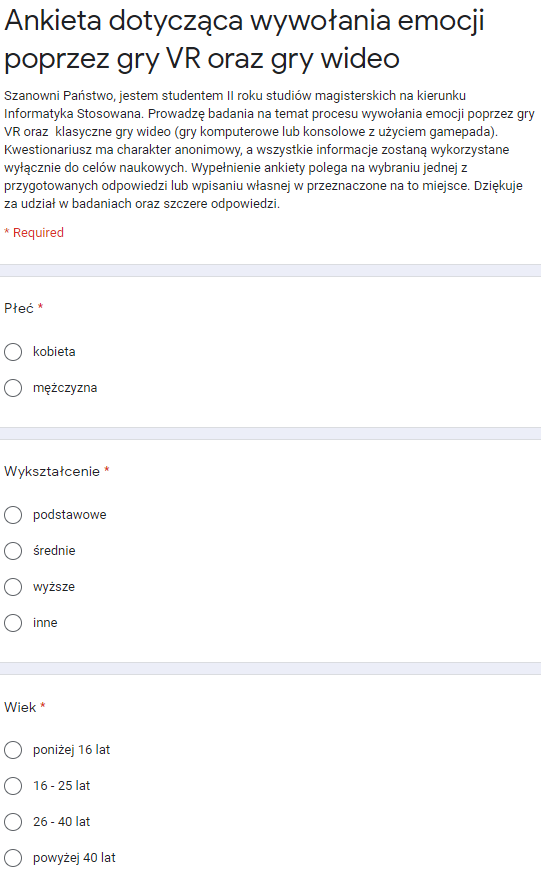
\includegraphics[width=0.7\textwidth]{images/ankieta1.PNG}
\end{figure}
\begin{figure}
	\centering
	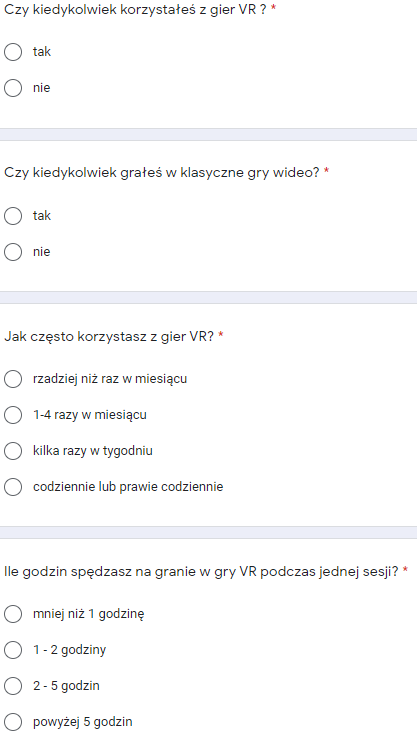
\includegraphics[width=0.7\textwidth]{images/ankieta12.PNG}
\end{figure}
\begin{figure}
	\centering
	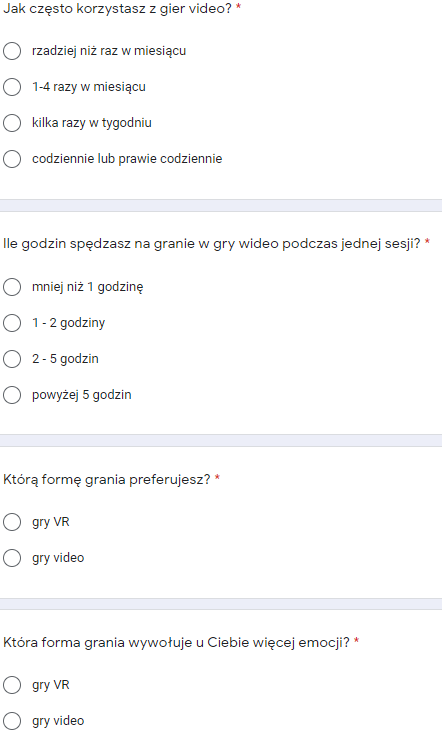
\includegraphics[width=0.7\textwidth]{images/ankieta123.PNG}
\end{figure}
\begin{figure}
	\centering
	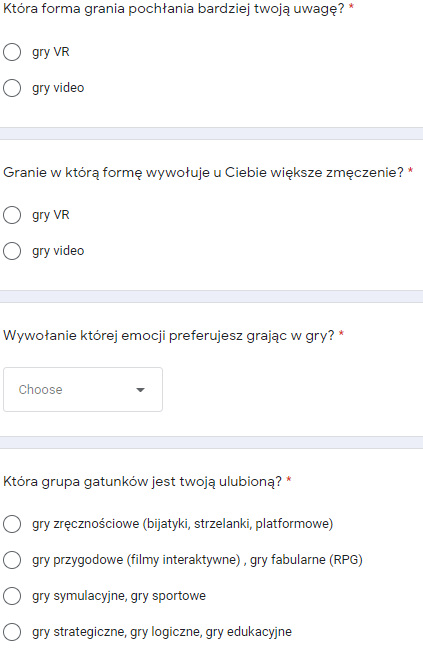
\includegraphics[width=0.7\textwidth]{images/ankieta1234.PNG}
\end{figure}
\begin{figure}
	\centering
	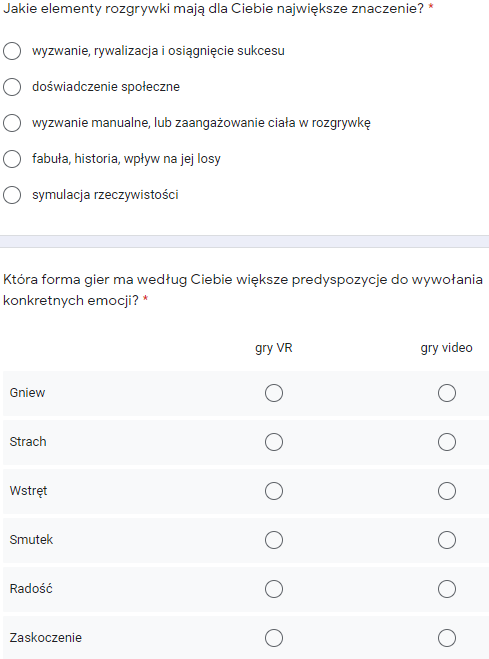
\includegraphics[width=0.7\textwidth]{images/ankieta12345.PNG}
\end{figure}
\begin{figure}
	\centering
	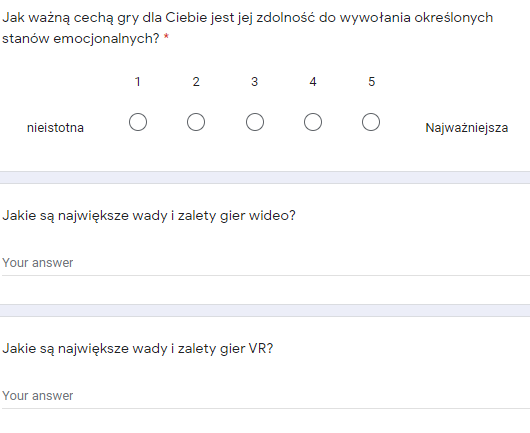
\includegraphics[width=0.7\textwidth]{images/ankieta123456.PNG}
\end{figure}


\end{document}

% % OLD 


% \documentclass{lib/uekthesis}
% \usepackage{lib/uekthesis}


% %####################################################################
% % INFORMACJE O PRACY DYPLOMOWEJ
% %####################################################################

% % tytuł pracy dyplomowej
% % \globalFullTitle{Analiza wirtualnej rzeczywistości jako medium do wywołania emocji na przykładzie gier.}

% \globalFullTitle{Wykorzystanie gier jako medium do wywołania określonych emocji - porównanie gier wideo i gier z wykorzystnaiem wirtualnej rzeczywistości.}

% % typ pracy, promotor
% \globalThesisType{Praca magisterska}
% \globalUnderTheSupervisonOf{Promotor}
% \globalSupervisor{Prof. UEK dr hab. Grażyna Paliwoda-Pękosz}

% % autor pracy
% \globalFullAuthor{Bartłomiej Hałdaś}

% % kierunek i specjalność studiów
% \globalDegreeprogramme{Kierunek: Informatyka Stosowana\\Specjalność: systemy inteligentne}

% % nazwa uniwersytetu
% \globalFullUniversity{Uniwersytet Ekonomiczny w Krakowie}

% % wydział, kolegium, instytut
% \globalDepartment{Kolegium Nauk o Zarządzaniu i Jakości\\Instytut Zarządzania}

% % miejscowość i rok
% \globalCity{Kraków}
% \globalYear{2020}



% %####################################################################
% % STRUKTURA PRACY DYPLOMOWEJ
% %####################################################################

% \begin{document}

% % strona tytułowa
% \titlepages

% % spis treści
% \tableofcontents

% % rozdziały pracy 
% \chapter*{Wstęp}
\label{chap:wstep}
\addcontentsline{toc}{chapter}{Wstęp}

Komputery nie służą już człowiekowi tylko jako narzędzie pracy z wysoką mocą obliczeniową, ale także dostarczają rozrywki wysokiej jakości bez potrzeby wychodzenia z domu. Gry pozwalają na aktywne doświadczenie, które może wyzwolić więcej emocji, a co za tym idzie więcej rozrywki niż media pasywne, dzięki narzędziom wykorzystywanym przez ich projektantów i twórców. 

Ludzie doświadczają rozmaitych emocji podczas grania w gry i jest to główny powód, który przyciąga miliardy graczy przed monitory w ciągu każdego roku. Gry wywołują różne stany emocjonalne u odbiorcy - różne typy gier są więc popularne wśród różnych odbiorców. Nie ma uniwersalnego doświadczenia, które zaspokoiłoby potrzeby każdego gracza, ale wszystkie pozycje mają wspólny mianownik, a mianowicie wywołanie konkretnego stanu u odbiorcy. Żadne inne medium nie oferuje takiej mocy transformacji jednostki na poziomie indywidualnym i społecznym, co jest możliwe dzięki dużej immersji przy równoczesnej możliwości wcielenia się w postać. Projektanci gier nadal przesuwają granice, pozwalając na coraz lepszą eksplorację świata oraz postaci, w które wciela się gracz.

Celem niniejszej pracy jest przybliżenie czytelnikowi czym jest technologia wirtualnej rzeczywistości (ang. Virtual Reality - VR), opisanie procesu powstania emocji oraz narzędzi wykorzystywanych do ich wywołania w grach oraz zbadanie jakimi zdolnościami do wywołania konkretnych emocji cechują się gry VR i gry wideo.  W toku badań własnych autora pracy udzielone zostaną odpowiedzi na następujące pytania badawcze: 

\begin{enumerate}
   \item Jaka jest charakterystyka graczy preferujących gry wideo, a jaka preferujących gry VR?
   \item Czym charakteryzuje się rozgrywka w gry typu VR, a czym w gry wideo?
   \item Czy emocje w grach są pożądane z perspektywy graczy oraz jaki jest związek pomiędzy platformą a wywołanymi emocjami?
\end{enumerate}

W tym celu przeprowadzono badania za pomocą kwestionariusza ankiety wśród osób mających styczność z grami wideo oraz technologią wirtualnej rzeczywistości.

Praca składa się z czterech rozdziałów. W pierwszym rozdziale scharakteryzowana zostaje technologia wirtualnej rzeczywistości, przybliżona zostaje jej historia oraz ewolucja na przestrzeni lat. Drugi rozdział definiuje pojęcie emocji, przedstawia jej funkcje oraz opisuje przebieg jej powstania u człowieka poprzez omówienie całego procesu: od oceny poznawczej aż po wykonanie działania. W kolejnym rozdziale zaprezentowano klasyfikację emocji oraz ukazanie jej związku z grami. Szczegółowo opisane zostają narzędzia wykorzystywane do wywołania emocji w grach oraz różnice między grami a innymi mediami pod względem wywołania emocji. W rozdziale czwartym zaprezentowano wyniki badań autora pracy. Scharakteryzowana została grupa badawcza, przedstawiono i przedyskutowano wyniki badań oraz udzielono odpowiedzi na sformułowane powyżej pytania badawcze.
% \chapter{Wirtualna rzeczywistość}
\label{chap:pierwszy}



%-------------------------------------------------------
\section{Wprowadzenie}

Interfejs, bo tak nazwana jest płaszczyzna, na której dochodzi do komunikacji między człowiekiem a komputerem, przez wiele lat przechodziła ewolucje – począwszy od wiersza poleceń, poprzez interfejs graficzny, a skończywszy na bezpośredniej komunikacji na poziomie mózg-komputer. Użytkownicy pierwszych interfejsów musieli ówcześnie posiąść wiedzę na temat ich obsługi, gdzie przykładem może być konieczność zaznajomienia się ze składnią tekstową i komendami wykorzystywanymi w danym systemie operacyjnym. Dziś coraz częściej używane są komunikaty przekazane przez człowieka w naturalny i intuicyjny sposób, takie jak gesty wykonywane na ekranach dotykowych smartfonów palcami dłoni, komendy głosowe oraz gesty wykonywane przy pomocy ciała, rozpoznawalne przez kamery i czujniki ruchu  \citep{virtualtech, virtualspeech}.

Za finalny etap ewolucyjny  uważa się całkowitą naturalizację interfejsu – co można częściowo zaobserwować na przykładzie wirtualnej rzeczywistości. Pozwala ona na skrócenie dystansu pomiędzy maszyną a człowiekiem dzięki rozszerzeniu jego zmysłów: słuchu, dotyku i wzroku przy wykorzystaniu technologii informatycznej co pozwala na wykreowanie pewnej wizji rzeczywistości, jednakże w świecie wirtualnym. W ciągu następnych dekad możemy spodziewać się znaczących zmian w naszych działaniach związanych z pracą, rozrywką i komunikacją, a wszystko dzięki rozwojowi wirtualnej rzeczywistości \citep{virtualspeech}.



\section{Definicja, części składowe i systematyzacja wirtualnej rzeczywistości}

Wirtualna rzeczywistość zdefiniowana pod względem funkcjonalności to świat syntetyczny i niestatyczny, czyli taki, który reaguje na dane wejściowe użytkownika - gesty czy polecenia słowne. To z kolei, definiuje kluczową cechę wirtualnej rzeczywistości jaką jest interaktywność w czasie rzeczywistym. Interaktywność oraz siła z jaką VR absorbuje uwagę użytkownika, przyczyniają się do stworzenia uczucia ``zanurzenia'' w tymże świecie, czyli immersji \citep{virtualtech}.

Z powyższego opisu jasno wynika, że rzeczywistość wirtualna jest zarówno interaktywna (ang. interactive) jak i wciągająca (ang. immersive). Istnieje jednak trzecia składowa, bez której VR nie miałoby racji bytu, czyli ludzka wyobraźnia (ang. imagination). Zakres, w jakim aplikacja jest w stanie rozwiązać konkretny problem, czyli stopień, w którym symulacja działa prawidłowo, zależy więc w dużej mierze od ludzkiej wyobraźni. Rzeczywistość wirtualna jest zatem zintegrowanym trio immersji-interakcji-wyobraźni (ang. immersion, interaction, imagination), tak jak to pokazano na rysunku \ref{fig:triangle}, czyli trójkącie trzech ``I'' wirtualnej rzeczywistości \citep{virtualtech}.


\begin{figure}[h]
	\centering
	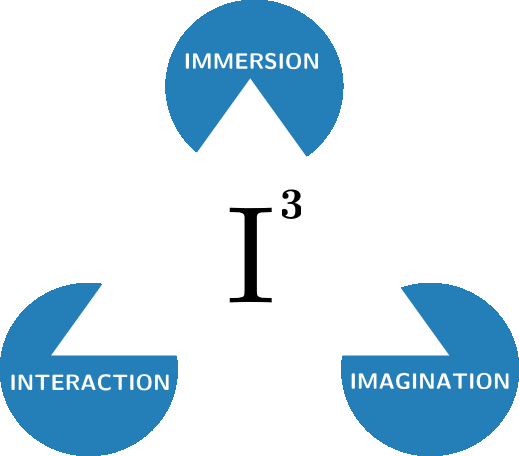
\includegraphics[width=0.6\textwidth]{images/triangle.png}
	\caption{Trzy składowe wirtualnej rzeczywistości.}
	\caption*{Źródło: \citep[s.~5]{virtualtech}.}
	\label{fig:triangle}
\end{figure}

Składowa jaką jest wyobraźnia, odnosi się do zdolności umysłu do postrzegania zasugerowanych, lecz nieistniejących rzeczy. Stąd trójkąt na rysunku 1 jest widoczny dla czytelnika, ale istnieje tylko w jego wyobraźni \citep{virtualtech}.

W celu ujednolicenia, każde kolejne odniesienie do wirtualnej rzeczywistości będzie bazowało na następującej definicji. Rzeczywistość wirtualna to immersyjna, interaktywna rzeczywistość symulowana komputerowo, która dzięki zaawansowanym urządzeniom wejścia i wyjścia tworzy złudzenie fizycznego środowiska, nie istniejącego w prawdziwym świecie fizycznym. Środowiska VR są zazwyczaj odcięte od tego świata w tym sensie, że cyfrowe środowiska, które powstają są całkowicie nowe - chociaż mogą być oparte na prawdziwych miejscach (takich jak szczyt Mount Everest) lub wymyślonych (takich jak podwodne miasto Atlantyda). Osoba korzystająca z wirtualnej rzeczywistości może rozglądać się po sztucznym świecie, poruszać się po nim, a także wchodzić w interakcję z wirtualnymi funkcjami i przedmiotami \citep{virtualfor}.

Rzeczywistość wirtualna jest często używana jako pojęcie ogólne dla wszelkiego rodzaju doświadczeń mocno absorbujących uwagę użytkownika, w tym wielu powiązanych terminów, takich jak rzeczywistość rozszerzona (ang. augumented reality, AR), rzeczywistość mieszana (ang. mixed reality, MR)  i rzeczywistość rozszerzona (ang. extended reality, XR) \citep{virtualfor}. W celu wyjaśnienia, czym dokładnie jest wirtualna rzeczywistość i czym różni się od pochodnych jej technologii, zostaną one umieszczone na skali Paula Miligrama, nazwanej kontinuum wirtualności, którą przedstawia rysunek \ref{fig:continuum}.

\begin{figure}[h]
	\centering
	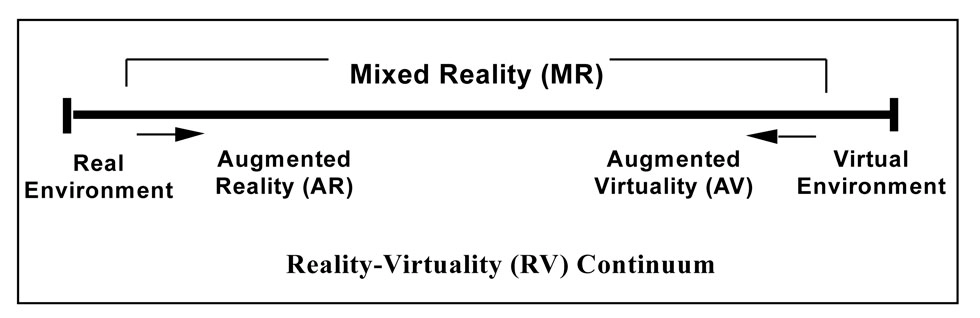
\includegraphics[width=1\textwidth]{images/2.spektrum.png}
	\caption{Kontinuum wirtualności.}
	\caption*{Źródło: \citep[s.~14]{virtualfor}.}
	\label{fig:continuum}
\end{figure}

Kontinuum wirtualności to skala używana do pomiaru poziomu rzeczywistości lub wirtualności konkretnych technologii. Na jednym końcu skali poziom jest w pełni realny, a na drugim całkowicie wirtualny. XR obejmuje pełne spektrum tej skali. Warto dodać, że MR oraz AR zostały rozdzielone, pomimo tego, że często określeń tych używa się synonimicznie. Niniejszy rozdział skupiać się będzie natomiast na głównych dwóch obszarach: VR i AR, które pokrywają większość scenariuszy związanych z rozszerzoną rzeczywistością.  Wirtualna rzeczywistość będzie używana w stosunku do kombinacji sprzętu i oprogramowania, które tworzy całkowicie nowe, cyfrowe symulacje. Natomiast rzeczywistość rozszerzona odnosić się będzie do dowolnego, istniejącego środowiska fizycznego jakie zostało wzbogacono o elementy cyfrowe, które z kolei nie muszą z nim bezpośrednio oddziaływać ani być interaktywne \citep{virtualfor}.

Rzeczywistość rozszerzona AR to jeden ze sposobów oglądania prawdziwego świata w sposób bezpośredni lub za pomocą urządzeń elektronicznych, takich jak kamera, która tworzy wizualizację świata fizycznego i ``rozszerza'' go za pomocą generowanych komputerowo danych graficznych, dźwiękowych i filmowych. AR różni się od VR tym, że AR powiększa istniejącą już fizycznie scenę o dodatkowe elementy, zamiast tworzyć całkowicie nową od podstaw. Pierwotnie uważano, że w AR dwa środowiska: fizyczne i syntetyczne nie mogą się ze sobą komunikować. W ostatnich latach definicja AR przybrała jednak inną formę i jest utożsamiana z rzeczywistością mieszaną, czyli taką, w której może zachodzić interakcja między światem rzeczywistym a cyfrowo rozszerzonym \citep{virtualfor}.

Porównanie zasady działania różnych typów rozszerzonej rzeczywistości przedstawia rysunek \ref{fig:vr-ar-mr}. Kolor zielony odwzorowuje obraz wirtualny, natomiast odcienie szarości przedstawiają świat fizyczny.


\begin{figure}[ht]
	\centering
	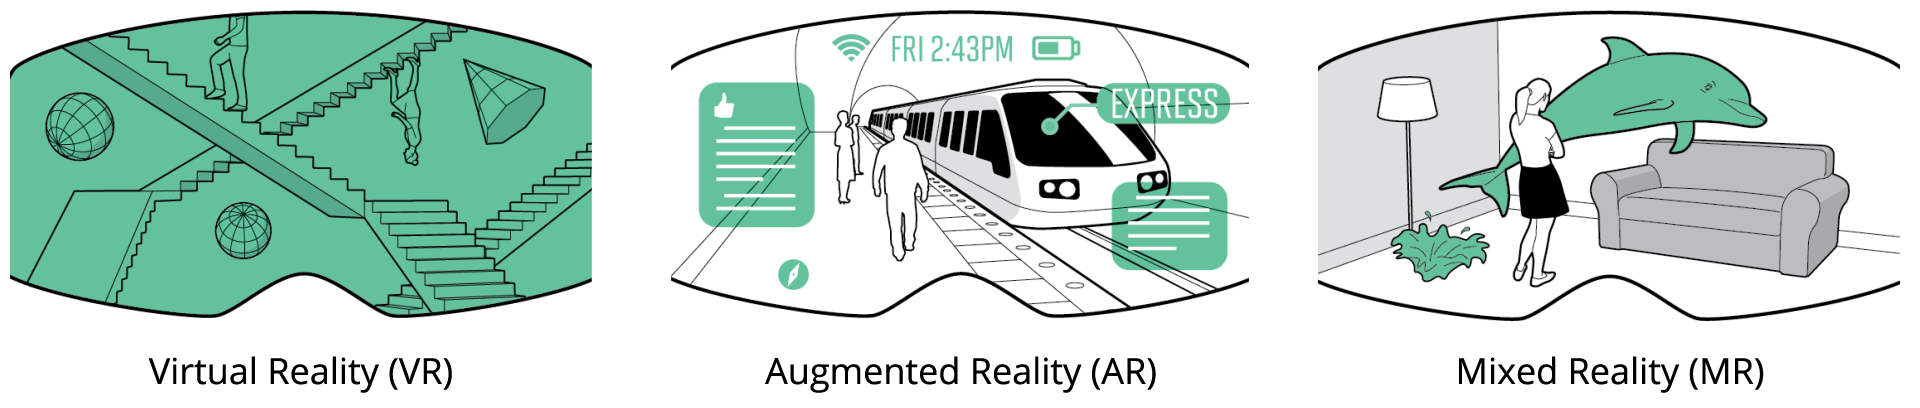
\includegraphics[width=1\textwidth]{images/1.xr-comparision.png}
	\caption{Porównanie VR, AR oraz MR.}
	\caption*{Źródło: https://www.cadcompany.nl/blog/vr-ar-en-mr-verschillen/}
	\caption*{Data dostępu: 15.02.2020.}
	\label{fig:vr-ar-mr}
\end{figure}

Rzeczywistość mieszana MR może przybrać różne formy i skłaniać się bardziej w stronę AR lub VR. Rzeczywistość mieszana, której podstawą jest AR, nie jest pasywnie nakładana na świat rzeczywisty, lecz zachowuje się jakby była częścią tego świata i wchodzi z nim w interakcje. Obiekty cyfrowe wyglądają tak, jakby istniały w prawdziwej przestrzeni. Przykładem może być umieszczona na stoliku do kawy cyfrowa rakieta, która rozpoczyna swoją misję kosmiczną lub cyfrowa piłka, która odbija się od ścian świata rzeczywistego. W innej wersji natomiast ukazuje się całkowicie cyfrowe środowisko lecz powiązane z otaczającymi użytkownika obiektami świata rzeczywistego, tak więc na przykład fizyczne, drewniane krzesła mogą mieć swoje odwzorowanie jako drzewa w cyfrowym świecie – jest to MR oparty na VR \citep{virtualfor}.

Rozszerzona wirtualność AV (z ang. Augumented virtuality), nazywana także połączoną rzeczywistością jest zasadniczo odwrotnością AR. Rozszerzona wirtualność dotyczy środowiska cyfrowego, w którym istnieje pewna integracja obiektów rzeczywistych poprzez strumieniowe przesyłanie video do środowiska wirtualnego lub tworzenia cyfrowej reprezentacji 3D istniejącego obiektu fizycznego \citep{virtualfor}.



%-------------------------------------------------------
\section{Ewolucja wirtualnej rzeczywistości}


%-------------------------------------------------------
\subsection{Narodziny}

Biorąc pod uwagę VR jako narzędzie do tworzenia iluzji – przeniesienia użytkownika w miejsce, w którym nie jest fizycznie to jako tego najwcześniejszą próbę możemy traktować 360 stopniowe malowidła ścienne lub panoramiczne obrazy z XIX wieku. Ich celem było wypełnienie całego pola widzenia obserwatora, sprawiając przy tym, że czuł się on ``zanurzony'' w wydarzeniu lub scenie oddanej na malowidle \citep{interactivemedia}.

Badania opublikowane w 1838 roku przez Charlesa Wheatstone’a wykazały, że ludzki mózg przetwarza dwa dwuwymiarowe obrazy z każdego oka w jeden, pojedynczy obiekt o trzech wymiarach. Stąd oglądanie dwóch zdjęć (jedno widoczne dla jednego oka, a drugie – podobne lecz nieidentyczne dla drugiego) za pomocą stereoskopu zapewniało użytkownikowi poczucie głębi i zanurzenia. Późniejszy rozwój popularnego stereoskopu View-Master opatentowanego w 1939 roku, dało początek dzisiejszym goglom VR \citep{interactivemedia}.

Wirtualna rzeczywistość choć dopiero teraz zyskuje na popularności, nie jest wynalazkiem XXI wieku, a jej historia sięga lat 50 ubiegłego stulecia. Za ojca VR uważany jest operator filmowy Morton Heiling, który to w 1962 roku zaprezentował maszynę o nazwie ``Sensorama'', którego schemat widnieje na rysunku \ref{fig:sensorama1}, a zdjęcie zostało przedstawione na rysunku \ref{fig:sensorama2}.  Było to urządzenie mechaniczne, którego zadaniem było symulowanie jazdy motocyklem przez Nowy Jork \citep{determinants}. Doświadczenie to polegało na jeździe wyimaginowanym motorem podczas oglądania krótkich ujęć filmów z ulic Nowego Jorku. W celu zwiększenia realności całego doświadczenia, symulowano podmuchy wiatru, zmiany kierunku jazdy, hałas oraz zapachy spotykane w mieście – od spalin po nowojorską pizzę, w zależności od miejsca, w jakim aktualnie znajdował się użytkownik. W systemie Sensorama brakowało jednak głównego elementu nowoczesnego systemu rzeczywistości wirtualnej: reakcji opartej na działaniach użytkownika \citep{virtualdev}.


\begin{figure}[ht]
    \centering
    \begin{minipage}{0.45\textwidth}
        \centering
        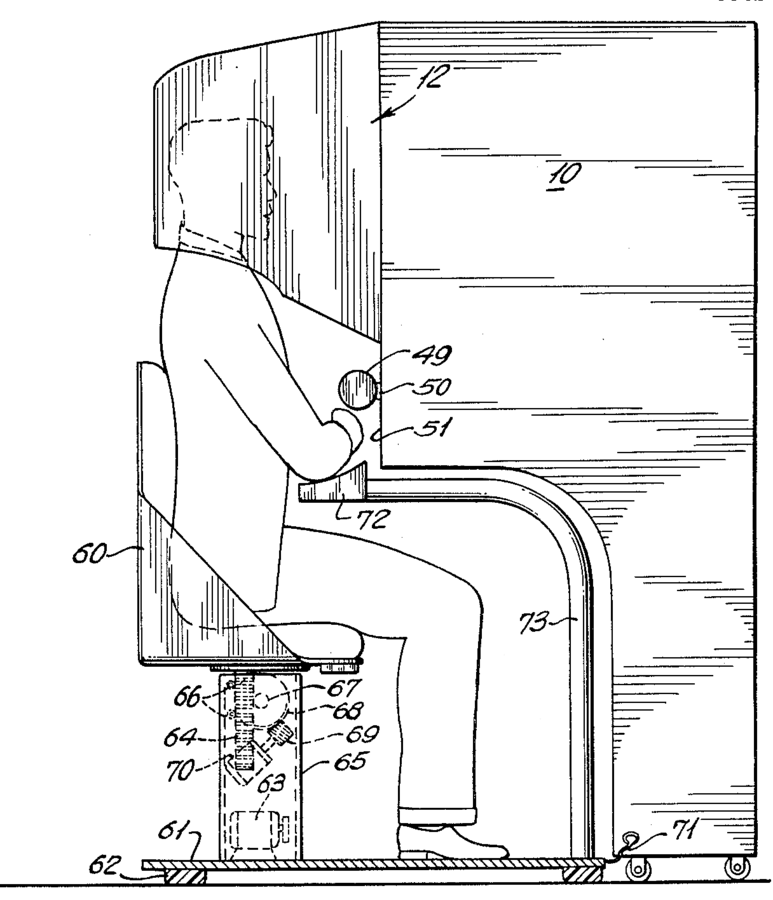
\includegraphics[width=0.9\textwidth]{images/sensorama1.png} % first figure itself
        \caption{Schemat Sensoramy w przekroju bocznym (zdjęcie z patentu USA nr #3050870).}
        \caption*{Źródło: https://smattes.com/article
        /47/sensorama}
        \caption*{Data dostępu: 15.02.2020.}
        \label{fig:sensorama1}
    \end{minipage}\hfill
    \begin{minipage}{0.45\textwidth}
        \centering
        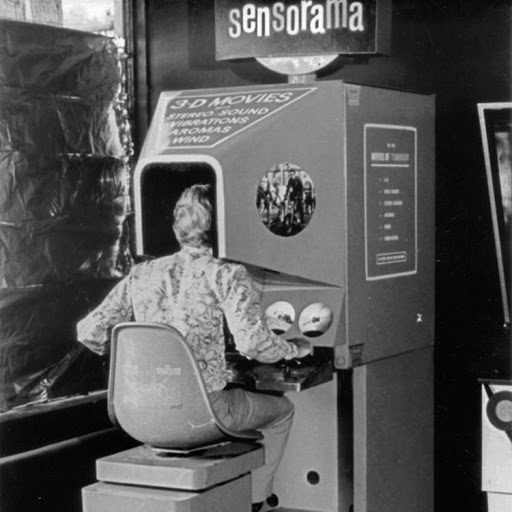
\includegraphics[width=0.9\textwidth]{images/sensorama2.jpg} % second figure itself
        \caption{Sensorama - pierwsze urządzenie wykorzystujące VR.}
        \caption*{Źródło: https://www.researchgate.net
        /figure/Sensorama-From-web-page-
        InventorVR-retrieved-in-March-2014-from\_fig1\_263388241}
        \caption*{Data dostępu: 15.02.2020.}
        \label{fig:sensorama2}
    \end{minipage}
\end{figure}


%-------------------------------------------------------
\subsection{Rozwój}

Krótko po wynalezieniu Sensoramy, Heilig opatentował również maskę Telesphere, pierwszy w historii wyświetlacz montowany na głowie HMD (ang. head-mounted display), czyli tak zwany hełm wideo, który zapewniał stereoskopowy obraz 3D i dźwięk stereo. Zestaw ten był nadal nieinteraktywny, choć zewnętrznie przypominał dzisiejsze okulary VR \citep{website:virtualspeech}.

W roku 1968 Ivan Sutherland, profesor Harvardu w dziedzinie informatyki, wynalazł pierwszy interaktywny hełm wideo, który był podłączony do komputera. System Sutherlanda to duży sprzęt, podwieszany przy suficie, który nosił nazwę ``Miecz Damoklesa''. Obejmował on hełm wideo oraz elementy, które mechanicznie śledziły głowę za pomocą szpulowych zwijanych kabli oraz program komputerowy, który w prosty sposób w formie trójwymiarowej generował prymitywne pokoje lub obiekty szkieletowe jak na przykład cząsteczka wody.  Sutherland w późniejszym czasie opracował zaawansowany sprzęt do renderowania grafiki w czasie rzeczywistym dla społeczności pilotów korzystających z symulatorów lotów, już jako  współzałożyciel Evans i Sutherland Computer Corporation (E&S) \citep{virtualdev}.


Po demonstracji Sutherlanda w laboratoriach uniwersyteckich, instytucjach rządowych i wojskowych, a później w sektorze komercyjnym, podjęto szereg prac badawczo-rozwojowych. W społeczności akademickiej badacz z University of Wisconsin, Myron Krueger eksperymentował z rozszerzoną rzeczywistością, czego wynikiem było powstanie systemu nazwanego ``Videoplace''. Systemy Kruegera również różniły się od pracy Sutherlanda tym, że wykorzystywał sygnały wejściowe z kamery wideo do śledzenia ruchów użytkownika. Videoplace było miejscem, w skład którego wchodziły zaciemnione pomieszczenia z zainstalowanymi na ścianach ekranami wideo, które otaczały użytkownika. Odbiorcy mogli zobaczyć wygenerowane przez komputer sylwetki naśladujące ich ruchy i działania - ruchy użytkowników były rejestrowane w kamerze i przenoszone na wirtualną postać. Ponadto użytkownicy różnych pokoi mogli wchodzić w interakcje z innymi użytkownikami w wirtualnym świecie, co powoli prowadziło do wniosków, że komunikacja w wirtualnym świecie jest możliwa, nawet jeśli dwie osoby nie są fizycznie blisko \citep{website:virtualspeech}.


W czasie, gdy Ivan Sutherland pracował nad projektem „Miecz Damoklesa”, inżynier wojskowy Thomas Furness opracowywał swój prywatny projekt - ``Super Kokpit''. Furness kontynuował prace nad projektem do lat osiemdziesiątych, w wyniku czego kokpit szkoleniowy był w stanie wyświetlać wygenerowane komputerowo mapy 3D, zdjęcia w podczerwieni i obrazy radarowe, a także dane samolotu w przestrzeni 3D w czasie rzeczywistym \citep{website:digitaltrends}.

W roku 1978 Massachusetts Institute of Technology (MIT) opracowało Aspen Movie Map, która znacząco przypominała dzisiejszą funkcję ``street view'' oferowaną przez Google Maps. Program ten pozwolił użytkownikowi na wirtualny spacer przez miasto Aspen (Kolorado) w trzech trybach: letnim, zimowym i wyświetlającym wielokąty. Doświadczenie to zostało stworzone na podstawie zdjęć z samochodu jadącego przez miasto. Chociaż projekt ten nie wykorzystywał komponentu hełmu wirtualnego,  w sposób innowacyjny wykorzystano interaktywność z perspektywy pierwszej osoby i ukazano w jak prosty sposób VR można wykorzystać do ``wirtualnego przeniesienia'' ludzi w inne miejsce na Ziemi \citep{website:digitaltrends}.

Rękawice do śledzenia palców dla VR, zwane rękawiczkami ``Sayre'' zostały wynalezione przez Daniela Sandina i Thomasa DeFanti. Rękawice były podłączone do systemu komputerowego i monitorowały ruchy dłoni za pomocą emiterów światła i fotokomórek w palcach rękawic. Kiedy użytkownik poruszał palcami, ilość światła padającego na fotokomórkę zmieniała się, co następnie przekształcało ruchy palców w sygnały elektryczne. Był to prekursor ``rękawic danych'', które stały się w późniejszym czasie ważną częścią wczesnej rzeczywistości wirtualnej \citep{website:virtualspeech}.

Pomimo prężnego rozwoju VR wciąż nie było terminu opisującego tę dziedzinę. Wszystko zmieniło się w 1987 roku, gdy Jaron Lanier, założyciel laboratorium programowania wizualnego (VPL), wymyślił termin ``rzeczywistość wirtualna''. W późniejszym czasie, dzięki swojej firmie VPL Research Jaron opracował gamę sprzętu do rzeczywistości wirtualnej, w tym Dataglove (wraz z Tomem Zimmermanem) i montowany na głowie wyświetlacz  EyePhone. Była to pierwsza firma, która sprzedawała gogle oraz rękawice do obsługi wirtualnej rzeczywistości. Miało to znaczący wpływ na rozwój w dziedzinie dotykowej rzeczywistości \citep{website:learng2, interactivemedia}. Rysunek \ref{fig:eyephone} przedstawia rękawice Dataglove oraz headset Eyephone podczas użytkowania.

\begin{figure}[ht]
	\centering
	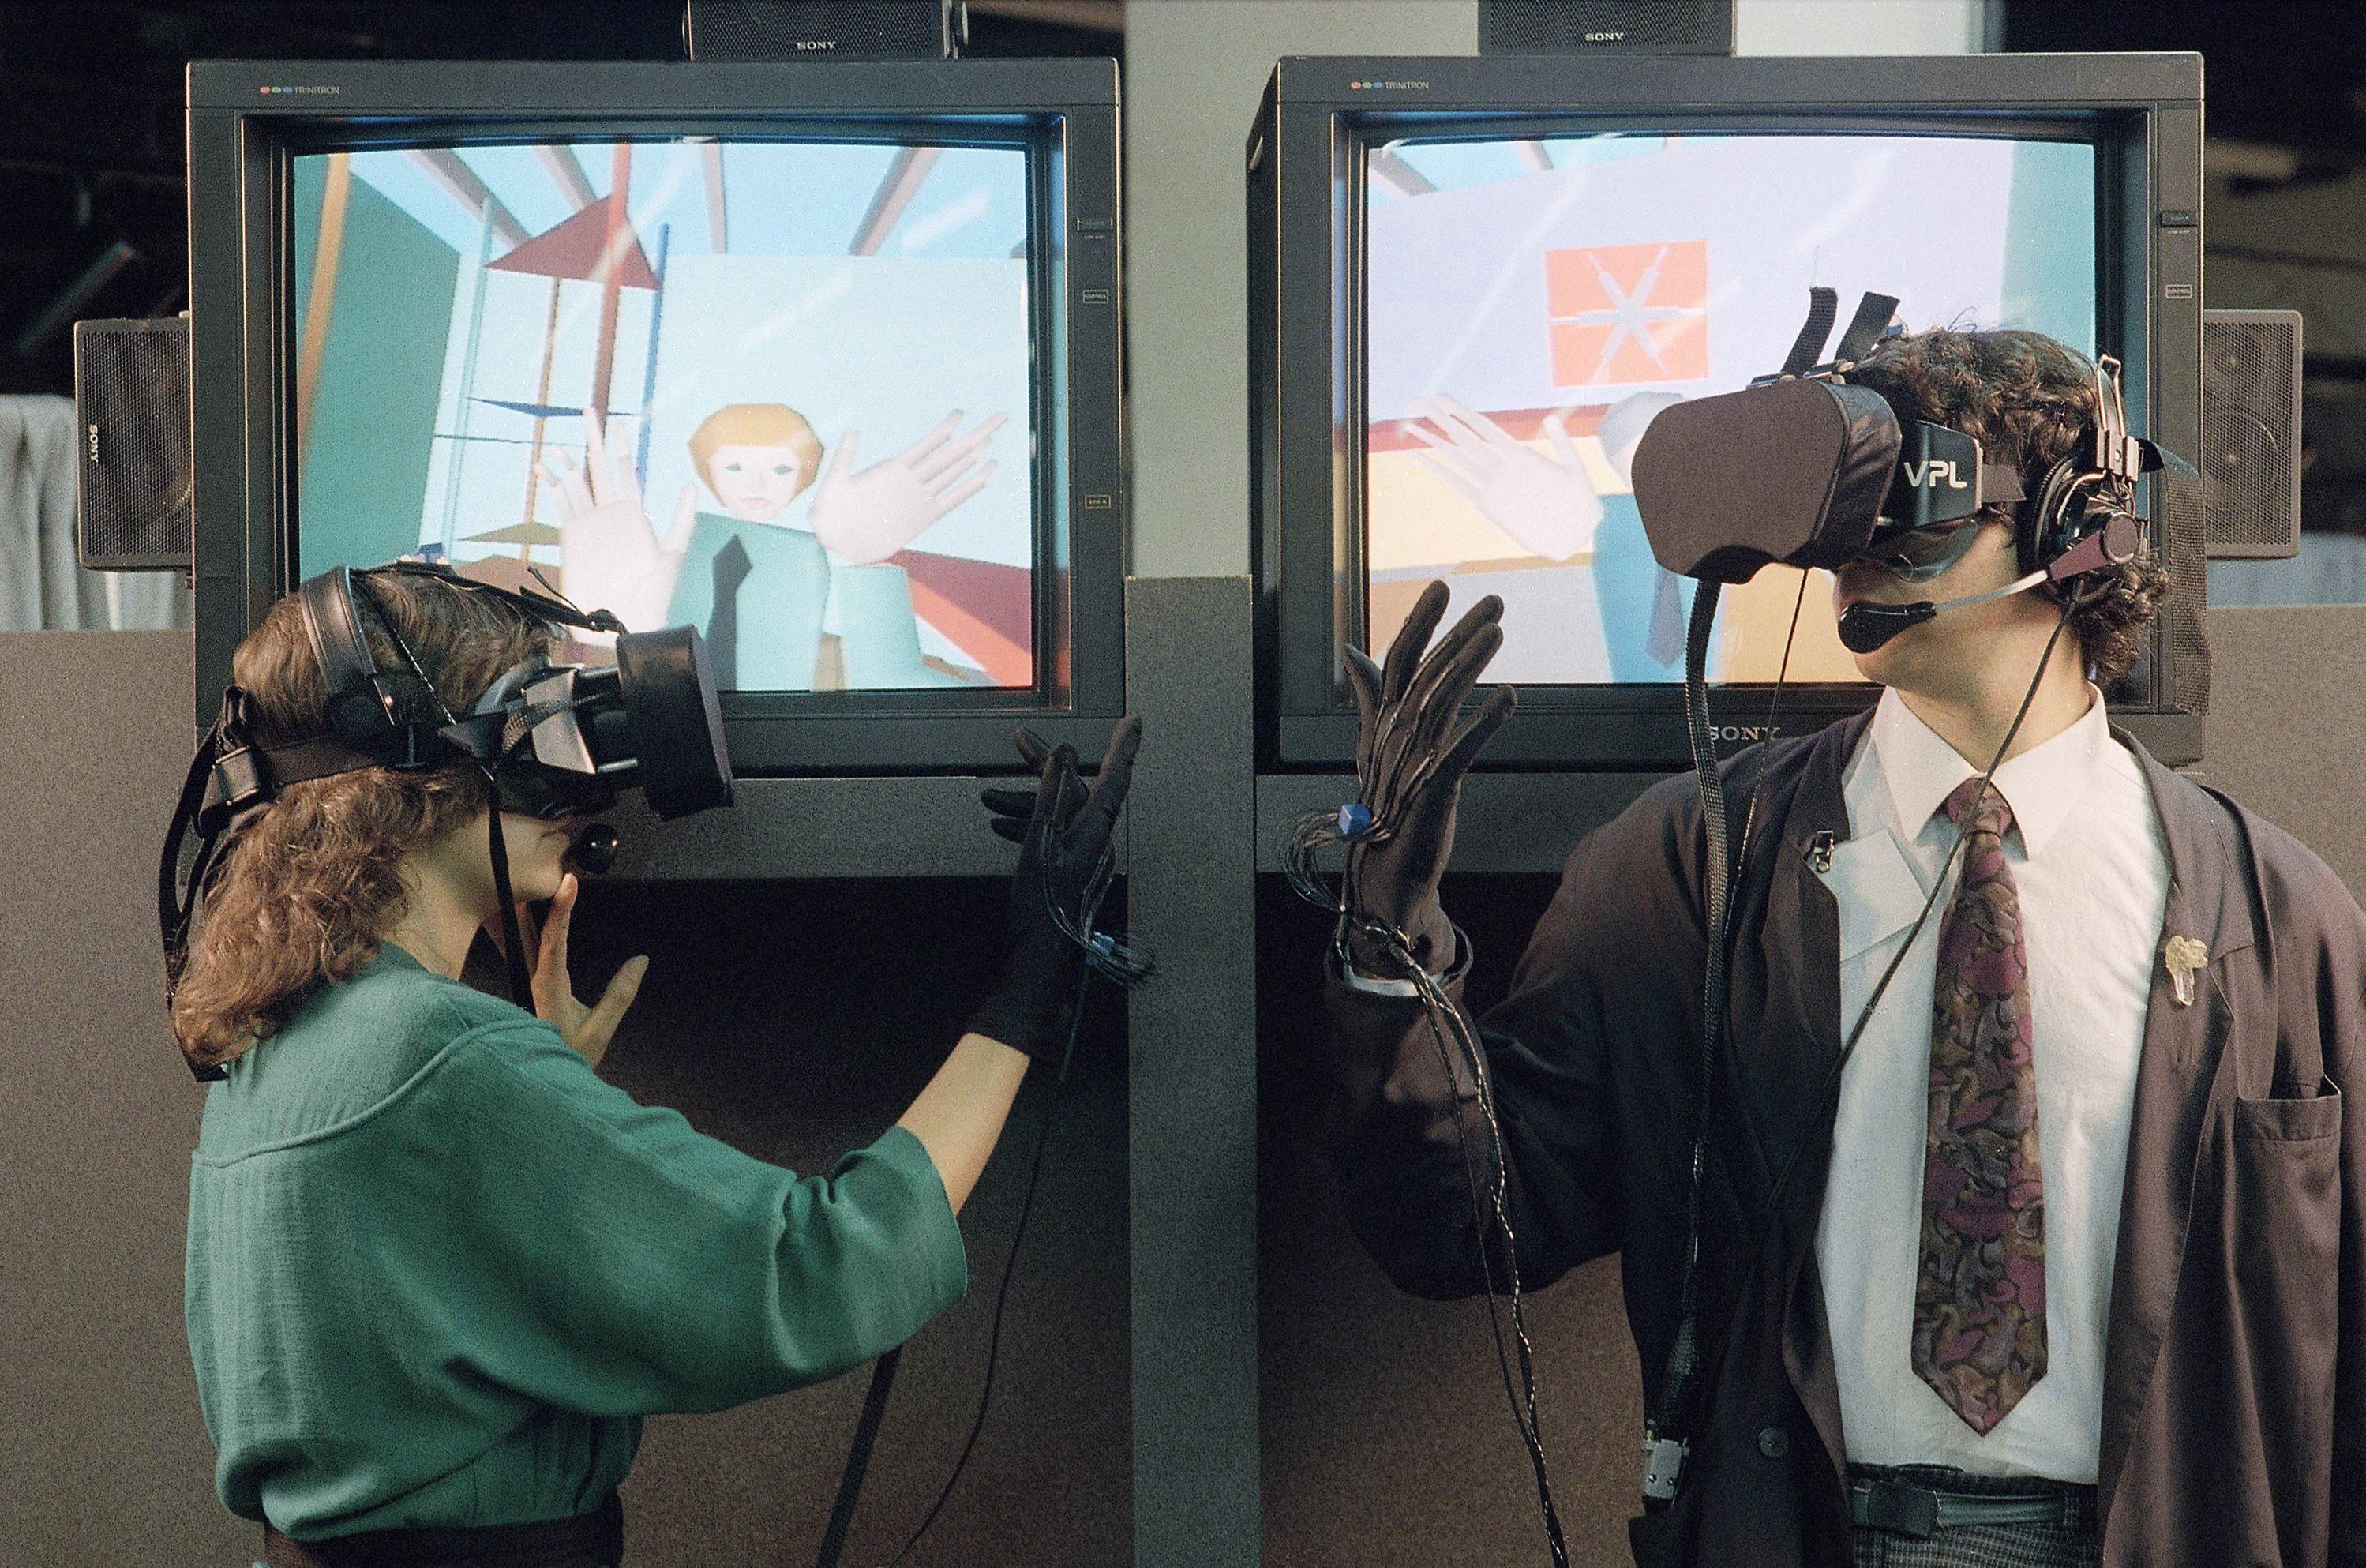
\includegraphics[width=0.7\textwidth]{images/jaron.jpg}
	\caption{Rękawice Dataglove oraz headset Eyephone w trakcie użycia.}
	\caption*{Źródło: https://flashbak.com/jaron-laniers-eyephone-head
	-and-glove-virtual-reality-in-the-1980s-26180/}
	\caption*{Data dostępu: 20.02.2020.}
	\label{fig:eyephone}
\end{figure}

Rok 1991 był przełomowy dla systemów VR dostarczających rozrywkę. Grupa Virtuality zaczęła dystrybuować automaty do gier VR o nazwie ``Virtuality'', w których gracze mogli grać w świecie gier 3D. Był to pierwszy masowo produkowany system rozrywki VR. Virtuality zawierała stereoskopowe okulary VR, które generowały obrazy 3D w czasie rzeczywistym. Niektóre z maszyn mogły być podłączone wspólnie, pozwalając przy tym na grę w trybie wieloosobowym \citep{website:virtualspeech}.

W 1993 SEGA ogłosiła, że pracuje nad zestawem słuchawkowym SEGA VR, który będzie dostępny dla ogółu społeczeństwa. Ten zestaw słuchawkowy miał być przeznaczony do gier zręcznościowych i konsoli Mega Drive. Wyglądał jak przyłbica dzięki wpływom popularnych wtedy filmów, takich jak RoboCop. W wizjerze umieszczono wyświetlacze LCD, a także słuchawki stereo i czujniki do śledzenia ruchu głowy. Jednak projekt ten nigdy nie został wydany, choć stworzono dla niego cztery gry. Jednym z wyjaśnień jakie ogłosiła firma SEGA, była ich obawa przed utratą zdrowia użytkowników, ponieważ efekt VR był zbyt realistyczny. Wydaje się to jednak mało prawdopodobne ze względu na ograniczoną moc obliczeniową w tamtych latach \citep{website:virtualspeech}.

W roku 1997 rozpoczęto terapie w leczeniu zespołu stresu pourazowego (ang. Posttraumatic Stress Disorder, PTSD) u weteranów wojennych. Do dnia dzisiejszego jest to nadal jeden z kluczowych obszarów leczenia i badań PTSD. Technologia VR dała terapeutom niezrównaną kontrolę nad tym, co pacjenci widzą i czego doświadczają \citep{interactivemedia}.


%-------------------------------------------------------
\subsection{Lata współczesne i prognozy na przyszłość}

Prawdziwy przełom nastąpił w roku 2010. Przedsiębiorca Palem Luckey był zawiedziony zestawami VR dostępnymi na rynku. Według jego opinii były zbyt drogie, ciężkie oraz miały małe pole widzenia, a opóźnienia miedzy interakcją użytkownika a odpowiedzią komputera były zbyt długie. Luckey zbudował serie prototypów zestawów VR, koncentrując się przy tym na stworzeniu taniego zestawu o niskim opóźnieniu, ale z dużym polem widzenia oraz wygodnym w użytku. Jego jednostka szóstej generacji została nazwana Oculus Rift Development Kit 1 i zaoferował ją na platformie Kickstarter, pozwalającej na finansowanie przez użytkowników projektów z różnych dziedzin życia. Zbiórka pieniędzy na rzecz projektu odniosła ogromny sukces, przynosząc 2,4 miliona dolarów, prawie 980 procent pierwotnego celu. Co ważniejsze, kampania Kickstarter przyczyniła się do wzrostu zainteresowania VR na rynku konsumenckim do rekordowego poziomu \citep{virtualfor}. Porównanie pierwszej i najnowszej wersji zestawu Oculus przedstawiono na rysunku \ref{fig:rift} i rysunku \ref{fig:quest}.

\begin{figure}[ht]
    \centering
    \begin{minipage}{0.45\textwidth}
        \centering
        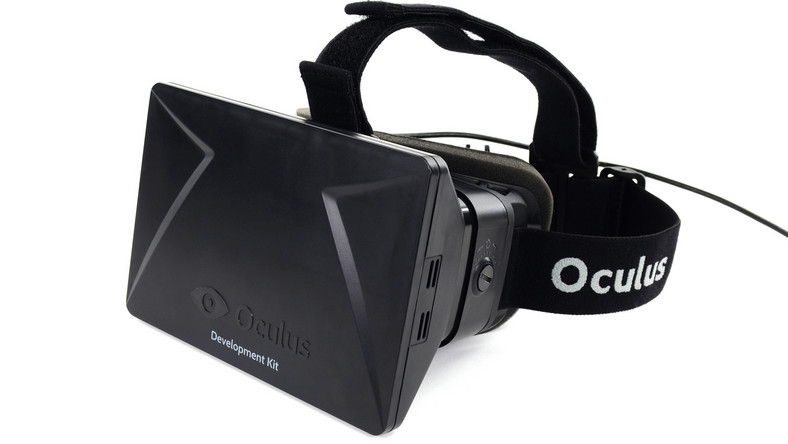
\includegraphics[width=0.9\textwidth]{images/oculusold.jpg} % first figure itself
        \caption{Zestaw Oculus Rift Development Kit 1 z roku 2010.}
        \caption*{Źródło: https://www.ifixit.com/Device
        /Oculus\_Rift\_DK1}
        \caption*{Data dostępu: 25.02.2020.}
        \label{fig:rift}
    \end{minipage}\hfill
    \begin{minipage}{0.45\textwidth}
        \centering
        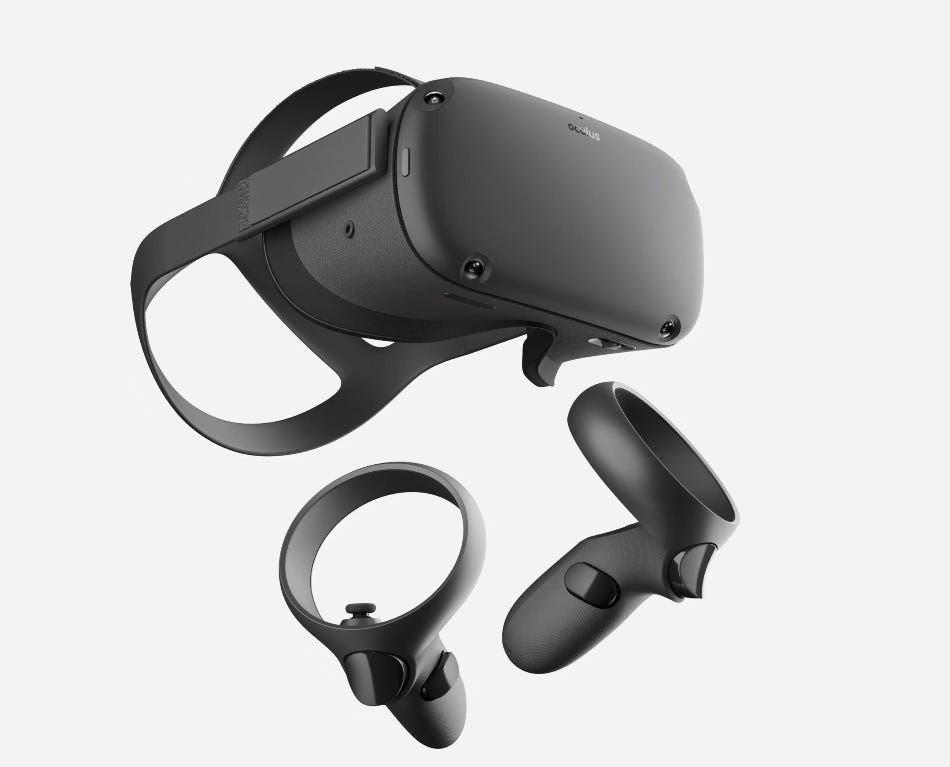
\includegraphics[width=0.9\textwidth]{images/oculusquest.jpg} % second figure itself
        \caption{Zestaw Oculus Quest z roku 2019.}
        \caption*{Źródło: https://i.insider.com/
        5df1222cfd9db23851669bd2?width=1100&
        format=jpeg&auto=webp}
        \caption*{Data dostępu: 25.02.2020.}
        \label{fig:quest}
    \end{minipage}
\end{figure}

Firma została zakupiona przez Facebook za 2 miliardy dolarów w 2014 roku. Decyzja Luckeya o sprzedaży firmy przed wysyłką prototypów do użytkowników, którzy zapłacili przez serwis Kickstarter wzbudziła kontrowersję, jednak był to dla historii VR decydujący moment, uznawany za przełomowy względem wzrostu popularności tej technologii \citep{virtualfor}.

Setki firm pracują nad własnymi zestawami VR: należą do nich liderzy rynku; wielkie koncerny takie jak HTC, Google, Apple, Amazon, Sony, Samsung oraz wiele innych, pomniejszych kompani. Prowadzi to do coraz większego popularyzowania tej technologii, jej szybkiego rozwoju przy jednoczesnym spadku cen, które są kluczowe dla rynku konsumenckiego i czynią  zaawansowaną technologię codziennym produktem w życiu człowieka. Dzisiejsze zestawy VR cechują się mobilnością i niewygórowanymi cenami, dzięki czemu mogą z nich skorzystać przeciętni użytkownicy innych powszechnie używanych technologii \citep{website:virtualspeech}.

Aktualne liczbę graczy ogółem na świecie szacuje się na ponad 2.5 miliarda, z czego gracze VR to tylko 171 milionów \citep{website:gameindustry, website:vrstats}. Liczba ta ciągle rośnie, a to za sprawą wciąż rozwijającej się technologii VR. Największą wadą VR jest brak rozbudowanych, wysokobudżetowych gier, lecz i to ulega zmianie. Wydanie jednej, dobrze przyjętej przez graczy produkcji może znacząco zmienić liczbę aktywnych graczy. Przykładem może być wydanie gry ``Half-life: Alyx'', kiedy w ciągu jednego miesiąca odnotowano przyrost 1 miliona nowych użytkowników VR \citep{website:alyx}.

VR coraz prężniej się rozwija i zyskuje coraz to nowe zastosowania w codziennym życiu człowieka, co można zawdzięczać finansowaniu tej technologii przez największe koncerny branży technologicznej. VR na przestrzeni ostatnich lat postrzegany był głównie jako forma rozrywki, mimo to ma wiele innych, potencjalnych zastosowań, m.in. w architekturze, wojsku czy medycynie. Jak dotąd, znana we współczesnym wydaniu wirtualna rzeczywistość 50 lat temu nawet nie istniała, ale biorąc pod uwagę jak prężnie rozwinęła się przez ostatnie kilka lat oraz jak wielki kapitał jest w nią inwestowany, zdawać się może, że kolejne etapy rozwoju będą coraz bardziej ekscytujące i interesujące dla fanów nowej technologii \citep{website:learng2, website:zastosowanievr}.


% \chapter{Emocje - geneza i funkcje}
% \chapter{Emocje w grach - VR w aspekcie neuropsychologicznym}
\label{chap:drugi}



%-------------------------------------------------------
\section{Wprowadzenie}

Emocje towarzyszą człowiekowi w codziennym życiu. Są uważane za uosobienie tego, co czyni nas ludźmi, jednak wydają się być przy tym bardzo podobne do reakcji innych zwierząt na pewne, określone bodźce \citep{website:emotion}.

Sztuka, przemysł rozrywkowy, reklama - wszystkie te dziedziny bazują w dzisiejszych czasach na wywoływaniu emocji u odbiorcy. Każde z tych mediów posiada swoje mocne i słabe strony, jeśli chodzi o wywoływania emocji. Skupiając się na emocjach wywoływanych przez gry, można stwierdzić, że opierają się one na tych samych, sprawdzonych metodach zaczerpniętych z filmów i powieści. Poprzez immersję, gry pozwalają na większe zatracenie się w wirtualnym świecie, co daje możliwość twórcom na wykreowanie unikalnego doświadczenia dla użytkownika, które nie byłoby możliwe do uzyskania używając innych środków przekazu. Gry wideo to wciąż ewoluujące medium, którego potencjał jest nadal badany \citep{button}.

\section{Definicja i klasyfikacja emocji}
Na wstępie należy sklasyfikować i rozróżnić występujące u ludzi stany emocjonalne: afekty, emocje i nastroje. Afekt to ogólny termin, obejmujący szeroki zakres uczuć, których ludzie doświadczają - jest to ogólna koncepcja pokrywająca zarówno emocje i nastroje. Emocja to pojęcie, które jest, ale również było w historii psychologii trudne do zdefiniowania. Poniższa definicja emocji oparta jest głównie o dzieło Frijdy z 1986 roku, czyli jedno z najnowocześniejszych zbiorów badań nad emocjami \citep{oatly}.

``Emocja spowodowana jest zazwyczaj przez świadome lub nieświadome wartościowanie przez podmiot jakiegoś zdarzenia jako istotnego dla jakiejś ważnej dla niego sprawy lub celu; emocja odczuwana jest jako pozytywna, jeżeli zdarzenie sprzyja tej sprawie, a jako negatywna, jeżeli ją utrudnia. Rdzeniem emocji jest gotowość do działania i podsuwanie planów; konkretna emocja nadaje priorytet jednemu lub kilku rodzajom działania, narzucając poczucie ich pilności - może więc zakłócać alternatywne procesy umysłowe lub działania albo rywalizować z nimi. Odmienne typy gotowości tworzą odmienne wyjściowe zarysy relacji z innymi. Konkretna emocja jest zazwyczaj doznawana jako odrębny typ stanu umysłowego, któremu niekiedy towarzyszą lub następują po nim zmiany somatyczne, akty ekspresji i działania'' \citep[s.~95]{oatly}.

Nastroje rozróżniane są od emocji głównie pod względem długości trwania. Pomimo braku definicji typowego czasu jaki trwa emocja bądź nastrój, to nastrój trwa dłużej. Czas trwania stanu afektywnego to nie jedyne kryterium pozwalające na odróżnienie nastrój od emocji. Występowanie specyficznych wyrazów mimicznych przypisywane jest do emocji, natomiast nie są one charakterystyczne dla nastrojów. Nastroje mogą nasilać szansę na wzbudzenie konkretnych emocji - osoba poirytowana może szybciej odczuć gniew, a osoba w pozytywnym nastroju - szczęście. Emocje wynikają najczęściej z relacji człowieka z obiektem - są ukierunkowane, czyli skierowane na dany obiekt, choć można być nieświadomym ich przyczyn - na przykład człowiek może czuć gniew w stosunku do jakiegoś obiektu, choć może być nieświadomym do jakiego konkretnie. Nastrój zaś przypisywany jest jako nieukierunkowany stan afektywny, więc nie jest on skierowany na konkretny obiekt  \citep{ekman}.

Różnica, która wydaje się być najlepszym kryterium w odróżnieniu emocji od nastroju to gotowość do zmiany. Podczas wystąpienia emocji, człowiek wchodzi w stan gotowości na działanie, natomiast podczas wystąpienia nastroju człowiek najczęściej opiera się działaniu, które prowadziłoby do zmiany. Przykładem może być negatywny nastrój, w którym nie przyjmuje się zaproszenia na przyjęcie - przy czym również odrzuca stworzenie stanu, który wydaje się być przyjemniejszym od stanu aktualnego \citep{oatly}.

\section{Proces powstawania emocji}

\subsection{Fazy procesu powstania emocji}
Proces powstawania emocji jest złożony, każda emocja ma swoją przyczynę, przechodzi pewien proces, i rodzi konsekwencje. Emocje w ujęciu Frijdowskim można przedstawić jako ciąg faz zaprezentowany na rysunku \ref{fig:fazes}.

\begin{figure}[h]
	\centering
	
\includegraphics[width=0.9\textwidth]{images/diagram.png}
	\caption{Fazy procesu powstawania emocji.}
	\caption*{Źródło: opracowanie własne na podstawie \citep[s.98]{oatly}.}
	\label{fig:fazes}
\end{figure}

Powstanie emocji u człowieka rozpoczyna się od oceny poznawczej, następnie występuje wartościowanie kontekstowe zdarzenia, które przeobraża się w gotowość do działania. W zależności od emocji i okoliczności, ostatnią fazą jest zmiana psychologiczna, która może, lecz nie musi wystąpić z ekspresją i działaniem \citep{oatly}.

\subsection{Ocena poznawcza}
Jako ocenę poznawczą definiujemy rozpoznanie przez człowieka konkretnego zdarzenia, jako zdarzenia znaczącego dla osiągnięcia celu lub rozwiązania danego problemu. Ocenę poznawczą można podzielić na ocenę pierwotną i ocenę wtórną. Ocena pierwotna dotyczy oceny znaczenia zdarzenia dla danej osoby (zdarzenie bez znaczenia, sprzyjająco-pozytywne lub stresujące) \citep{oatly, website:teoriastresu}. Ocenie pierwotnej według Lazarusa  można przypisać trzy następujące cechy \citep{oatly}:

\begin{enumerate}
\item Ważność zdarzenia dla celu - emocja pojawi się tylko wtedy, kiedy wystąpi okoliczność mająca wpływ na cel lub problem.
\item Zgodność (lub niezgodność) z celem - postęp w osiągnięciu celu wywoła pozytywne emocje, natomiast regres emocje negatywne.
\item Wartość zdarzenia dla podmiotu - przykładem jest zaangażowanie poczucia własnej wartości, które może wywołać dumę lub gniew po zdarzeniu.
\end{enumerate}

Ocena wtórna zaś dotyczy szacowania własnych możliwości i radzenia sobie w sytuacji. Nie zawsze człowiek jest świadomy przyczyny wywołania u niego emocji jak i również faza oceny poznawczej przebiega najczęściej nieświadomie. Ocena czy coś jest ważne dla danego celu lub problemu przebiega mimowolnie w umyśle podmiotu. Aspekty emocji, które są zauważalne, występują w kolejnej fazie \citep{oatly, website:stres}.

\subsection{Wartościowanie kontekstowe}

Podczas doświadczania emocji ważne są również myśli podmiotu, które dotyczą przyszłych planów oraz sposobu w jaki należy poradzić sobie z okolicznościami jakie spowodowały wywołanie emocji. Jeśli w efekcie wywołania emocji, a zatem rezultacie wydarzenia może nastąpić zmiana priorytetów - zdarzenie to musi zostać dogłębnie przeanalizowane. Zatem emocje potrafią znacząco pobudzić aktywność umysłową polegającą między innymi na: zawężeniu uwagi, przywołaniu analogicznych sytuacji z przeszłości w celu skonfrontowania ich z aktualnym problemem czy tworzeniu przyszłych planów. Adaptacja do zmiany przez istoty ludzkie zależy od zrozumienia nowych wydarzeń i poczynaniu planów na podstawie tego co się wydarzyło. Kluczowymi są więc myśli zapoczątkowane emocjami, które decydują o ważności wydarzenia dla podmiotu oraz o tym, jakie należy wykonać działania aby zmienić stan rzeczy na bardziej korzystny. Znaczące jest także wnioskowanie o przyczynie wydarzenia wywołującego emocje, czyli tzw. atrybucja. Właśnie od atrybucji, czyli definiowanych przez ludzi przyczyn wydarzeń zależy charakter i nacechowanie emocji \citep{oatly}.

\subsection{Gotowość do działania}

Człowiek, poczynając od wieku 3 lat jest świadomy, że emocja może stworzyć problem, a co za tym idzie - wymaga działania, które go rozwiąże. Aktywność umysłowa od tego wieku najczęściej wyraża się w pytaniu ``Co z tym zrobić?''. Emocje można przyrównać do ścieżek pośród ludzkich działań. Ukazują to, co jest ważne, pozwalają skupić się na celu lub występującym problemie oraz są motywacją do ewentualnej zmiany biegu wydarzeń, czyli przyszłości - specyficzne emocje nadają priorytety konkretnym działaniom. Najczęściej gotowość do działania oraz plany dotyczą innych ludzi, choć nie jest to reguła. Gotowość do działaia według Frijdy, mówi o tym, że ta wywołana emocjami, będzie zawsze najważniejsza \citep{oatly, teorieemocji}.

\subsection{Ekspresja, zmiany somatyczne, działanie}

Plany, myśli oraz gotowość do działania podmiotu najczęściej są ukryte, ale istnieje sposób na rozpoznanie emocji występujących u ludzi. Najczęściej jest to obserwowane jako chwilowe zakończenie interakcji z otoczeniem przez podmiot, na rzecz interakcji z samym podmiotem, czego przykładem mogą być: napad płaczu, napad śmiechu lub paraliżujący napad strachu \citep{oatly}.

\subsubsection{Ekspresja}

Zakłada się, że emocje są stanami dyskretnymi lecz można je rozpoznać po przypisanej im konkretnej ekspresji - czyli działaniu lub procesie fizjologicznym np. poceniu, łzach. Ekspresja to coś, co zostało uzewnętrznione lub inaczej ``wyrażone'' (ang. expressed). Nie ma uniwersalnych odpowiedników stanów emocjonalnych dla wszystkich społeczeństw - są one kształtowe na różne sposoby dla różnych kultur i grup społecznych. Pomimo tychże różnic, sklasyfikowano pięć grup ekspresji niewerbalnych \citep{oatly}:
\begin{enumerate}
  \item Emblematy - inaczej gesty np. kciuk w górę oznaczający ``wszystko w porządku''. Popularne są również gesty nacechowane negatywnie np. wystawiony środkowy palec lub tzw. gest Kozakiewicza.
  \item Ilustratory - najczęściej połączone z informacjami przekazywanymi werbalnie. Ich intensywność wzrasta wraz ze stopniem pobudzenia emocjonalnego np. machanie rękami, zaciskanie pięści.
  \item Regulatory - przykładem może być kiwanie głową w celu podtrzymania płynności rozmowy.
  \item Przejawy afektu - ekspresje np. uśmiech, podniesienie lub zmarszczenie brwi.
  \item Adaptatory - przejawiają się samopielęgnacją np. dotykanie się po ramionach, co może oznaczać lęk lub konflikt wewnętrzny.
\end{enumerate}

\subsubsection{Zmiany somatyczne}

Jednym ze składników procesu są zmiany somatyczne. Stan somatyczny to: oddech, bicie serca, napięcie mięśni. Część z tych zmian jest wywoływanych podświadomie natomiast można je kontrolować. Oddech można spowolnić, a wykonując odpowiednie ruchy ciała możliwe jest także rozluźnienie mięśni. Dzięki kontrolowaniu zmian somatycznych można zintensyfikować lub osłabić emocje, czego przykładem może być branie wolnych i głębokich wdechów, które mogą wpłynąć na zmniejszenie poczucia lęku lub gniewu \citep{website:samokontrola}.

\subsubsection{Działanie}

Ściśle połączone z emocjami są działania i plany - emocje więc mają silny związek z zachowaniem podmiotu. Dzięki zmianom somatycznym organizm może zacząć wykonywać pewne czynności silniej lub szybciej. Przykładem może być gniew - generuje on zmiany fizjologiczne (pobudzenie pewnych mięśni), co przygotowuje podmiot do działania w szybszy sposób. Emocje jednak nie prowadzą bezpośrednio do zmian motorycznych realizujących konkretne plany, ale mają raczej charakter motywacyjny. Strach na przykład może być motywatorem do uniknięcia straty, tak więc następstwami wystąpienia emocji jest raczej zwiększenie skłonności do wykonania jakiegoś działania, niż samo wykonanie go \citep{ekman}.

\section{Funkcje emocji}

Emocje  lub coś ekwiwalentnego do nich są istotne dla złożonych, inteligentnych systemów, które mają różne motywy i działają w złożonym środowisku - nie tylko dla istot ludzkich. Są one ważne w otoczeniu, które nie jest w pełni poznane i nie jest możliwa jego pełna kontrola \citep{oatly}.

Emocje służą więc do uświadamiania podmiotowi jego aktualnego położenia w świecie i zaistniałej sytuacji, lecz nie są narzędziem, które przystosuje ten podmiot do bieżącej sytuacji. Tak więc można wywnioskować, że służą one adaptacji, ale funkcja ta nie jest wykorzystywana przy każdym przejawie wystąpienia emocji. Tak więc występujące emocje możemy sklasyfikować jako funkcjonalne oraz niefunkcjonalne \citep{ekman}.

Odczuwanie pozytywnych emocji ma charakter wzmocnienia - sygnalizują, że aktualnie wykonywane działania przybliżają jednostkę do osiągnięcia celu i motywują do kontynuacji tychże działań. Negatywne zaś wzbudzane są poprzez zdarzenia zagrażające osiągnięciu celów. Informują o  nieodzowności podjęcia konkretnych działań mających na celu zmianę aktualnego (złego) stanu rzeczy albo powstrzymują nadchodzące ewentualne nieprzychylne zmiany \citep{ekman}.

Innymi słowy emocje służą podtrzymaniu lub zmianie pewnych powiązań podmiotu z jego otoczeniem - nie są więc ukierunkowane na samo otoczenie. W dodatku emocje mogą regulować zasoby energii, które są wydawane w interakcji podmiotu z środowiskiem np. apatia towarzysząca smutkowi ułatwia przeżycie negatywnych wydarzeń w życiu poprzez zmniejszenie wrażliwości na doświadczanie bodźców emocjonalnych \citep{ekman}.

Kolejną funkcją emocji jest regulacja kontaktów społecznych, czyli innymi słowy regulacja zachowań pozwalająca na poprawne życie w społeczeństwie. Świadomość, że jakieś działanie może wywołać uczucie wstydu, może doprowadzić do pohamowania jego realizacji. Podobną, ale bardziej ogólną funkcje pełni wywołanie poczucia winy, które pozwala na uniknięcie kary za przewinienia \citep{ekman}.

Niektóre z przejawów emocji nie pełnią żadnej funkcji oraz zdają się być szkodliwe. Najlepszym przykładem zdają się być tęsknota i smutek. Czynią one życie bogatszym oraz skłaniają do refleksji, ale nie posiadają konkretnej funkcji. Emocje mimo to należy uznać za pożyteczny mechanizm, ale nie oznacza to, że każdy przejaw emocji jest użyteczny \citep{ekman}.

% \chapter{Emocje w grach}
\label{chap:trzeci}

\section{Wprowadzenie}

Grę komputerową definiujemy jako cyfrowe interaktywne doświadczenie dla jednego bądź wielu graczy. Od czasów powstania pierwszej gry wideo, to medium przeszło zauważalną transformację. W dzisiejszych czasach istnieje szeroki wachlarz typów gier wideo - od napiętego, filmowego doświadczenia pojedynczego gracza przedstawionego na rysunku \ref{fig:cod} (seria Call of Duty), po relaksujące doświadczenia wymagające cierpliwości (FarmVille) ukazane na rysunku \ref{fig:farm}. Gry wideo to ewoluujące medium, a ich potencjał wciąż jest badany. Toczą się gorące dyskusje na temat tego, czy gry można zaklasyfikować jako sztukę, czy nie. Słownik oksfordzki opisuje grę jako dzieło, które należy docenić przede wszystkim za piękno lub siłę emocjonalną \citep{button}.


\begin{figure}[ht]
    \centering
    \begin{minipage}{0.45\textwidth}
        \centering
        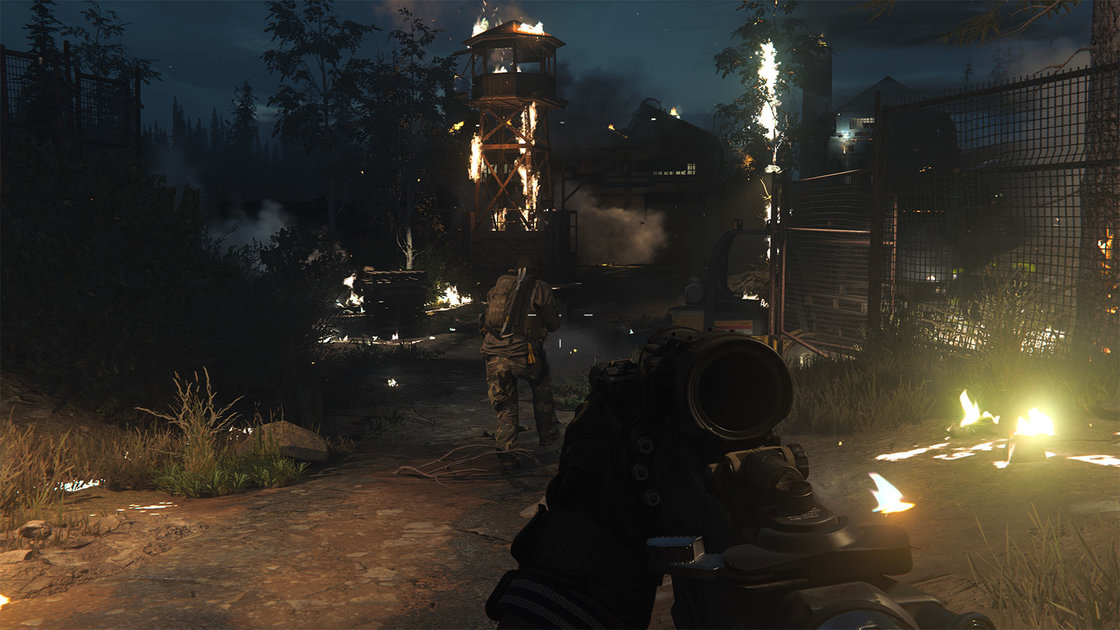
\includegraphics[width=1\textwidth]{images/cod.jpg} % first figure itself
        \caption{Widok z perspektywy pierwszej osoby z gry Call of Duty.}
        \caption*{Źródło: https://www.pocket-lint.com /games/reviews/activision/150364-call-of-duty-modern-warfare-review}
        \caption*{Data dostępu: 12.05.2020}
        \label{fig:cod}
    \end{minipage}\hfill
    \begin{minipage}{0.45\textwidth}
        \centering
        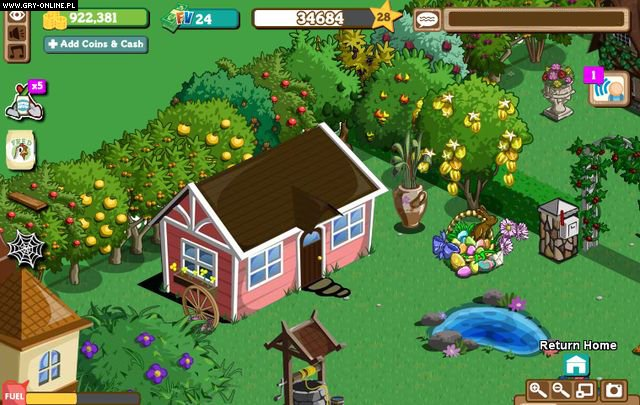
\includegraphics[width=1\textwidth]{images/farm.jpg} % second figure itself
        \caption{Widok gracza wraz z interfejsem użytkownika z gry FarmVille.}
        \caption*{Źródło: https://www.pocketgamer.com /games/023284/farmville-2-country-escape/screenshots/}
        \caption*{Data dostępu: 12.05.2020}
        \label{fig:farm}
    \end{minipage}
\end{figure}

Twórcy gier z reguły kopiują metody wywołania emocji z uznanych już wcześniej mediów - literatury i filmu. Gracze grają w gry dla doświadczenia pewnego przeżycia, a gry mają zdolność symulowania emocji w formie bliższej prawdziwemu życiu niż filmy czy książki. Mając to na uwadze, gry powinny mieć potencjał wywoływania silnych emocji, w połączeniu z konwencjonalnymi sposobami wykorzystanymi w wyżej wymienionych mediach, ale również bez ich wykorzystania. Jeśli chodzi o wywołanie emocji, potencjał gier wydaje się większy \citep{button, movesus}.

\section{Wymiary emocji}

Teorie emocji mówią, że ludzie są ewolucyjnie wyposażeni w ograniczony zestaw podstawowych emocji. Każda podstawowa emocja jest niezależna od innych w jej behawioralnych (związanych z zachowaniem), psychologicznych i fizjologicznych przejawach. Wyróżnia się sześć podstawowych emocji, a mianowicie \citep{colors}:
\begin{itemize}
  \item gniew,
  \item strach,
  \item wstręt,
  \item radość,
  \item smutek,
  \item zaskoczenie.
\end{itemize}

Większość teoretyków podziela pogląd, że emocje składają się z trzech głównych elementów: subiektywnego odczuwania, ekspresji i reakcji fizjologicznej. Jedne są motywacyjne i mają tendencję do wprowadzenia w stan motywacyjny lub tendencję do działania \citep{games}.

Istnieje możliwość określenia emocji, badając mimikę i reakcje fizjologiczne. Emocje można mierzyć również pośrednio za pomocą reakcji emocjonalnych. Badania pozwoliły na stworzenie modelu reakcji emocjonalnych.  Wymiarowa teoria emocji utrzymuje, że wszystkie emocje mogą znajdować się w dwuwymiarowej przestrzeni, jako współrzędne walencji oraz pobudzenia \citep{games}.

Jednym z często używanych modeli jest „kołowy model afektu” stworzony przez Russella w 1980 roku, który został przedstawiony na rysunku \ref{fig:spectrum}. Charakteryzuje on emocje w kategoriach dwóch wymiarów reakcji emocjonalnych, a mianowicie pobudzenia i walencji. Pobudzenie to fizjologiczny i psychologiczny stan bycia pobudzonym (aktywacja) lub brakiem pobudzenia (dezaktywacja) na bodźce. Walencja jest wewnętrznie pozytywnym (przyjemnym) lub negatywnym (nieprzyjemnym) uczuciem, które jest wywołane przez wydarzenie, przedmiot lub sytuację \citep{colors}.

\begin{figure}[h]
	\centering
	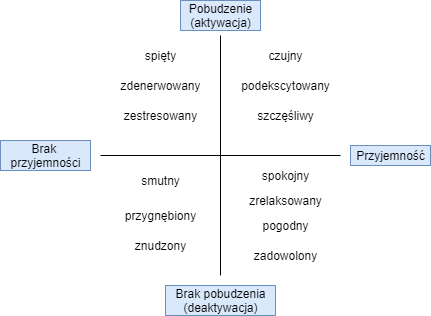
\includegraphics[width=0.85\textwidth]{images/diagram2.png}
	\caption{Kołowy model afektu stworzony przez Jamesa Russella. Oś pozioma odpowiada za walencję, a pionowa za stan pobudzenia.}
	\caption*{Źródło: opracowanie własne na podstawie \citep[s.1]{colors}.}
	\label{fig:spectrum}
\end{figure}


\section{Emocjonalne reakcje graczy}

Istnieje niewiele badań analizujących reakcje emocjonalne na gry z punktu widzenia doświadczenia użytkownika. Jednak niektóre badania dotyczyły jedynie negatywnie ocenianych emocji wywoływanych przez gry wideo, próbując rozwikłać ich potencjalne niekorzystne skutki. Badania były sprzeczne - jedne stwierdzały, że brutalne gry wideo wywołują wrogi afekt np. lęk, inne z kolei, że nie wywołują żadnego afektu. Ewentualnie niepokój może wynikać z obserwacji poziomu symbolicznej agresji, jaką samemu dokonuje się w grze. W odniesieniu do fizjologicznego komponentu emocji powszechnie wiadomo, że zadania wymagające wysiłku poznawczego lub aktywnego radzenia sobie wywołują pobudzenie emocjonalne, któremu towarzyszy m.in. przyspieszenie tętna. W badaniach nad psychofizjologiczną reaktywnością na stres, gry wideo były często wykorzystywane jako stresor. Kilka badań wykazało, że różne gry wideo wywołują znaczną reaktywność sercowo-naczyniową. Odkryto również, że dwuosobowa gra wideo na przykładzie „piłki nożnej” ma większy wpływ na tętno w porównaniu z grą wideo „trening squasha” przeciwko maszynie, co może sugerować, że sytuacja konkurencji społecznej związana z poprzednią grą powoduje zwiększone pobudzenie \citep{games}.


\section{Narzędzia wykorzystywane do wywołania emocji w grach}

\subsection{Awatar}

Awatar to byt, który wywodzi się z hinduskiej koncepcji boga wcielonego w różne istoty. Cyfrowy awatar to postać w wirtualnym świecie, która reprezentuje gracza. Bywają z góry zdefiniowane (tak jak postacie filmowe) lub istnieje możliwość  modyfikacji ich różnych cech: wyglądu, charakteru lub poziomu umiejętności \citep{glossary}.

Awatar jest często używany jako sposób na przeniesienie gracza do świata gry. Awatarów może być kilka i można ich używać na różne sposoby, ale łączy je to, że służą jako przedłużenie tożsamości gracza. Percepcja może wykroczyć poza świat realny, przenikając do wirtualnego i to samo dzieje się z tożsamością. Można to przyrównać do jazdy samochodem, kiedy podczas jazdy kierowca wyczuwa pozycje samochodu w przestrzeni, a ściślej określając do tzw. intuicyjnego ``wyczucia samochodu'' na przykład podczas parkowania - wtedy samochód staje się przedłużeniem ciała i jaźni \citep{gamefeel}.

Przedłużenie zmysłów gracza poprzez wcielenie się w postać pozwala zatracić się użytkownikowi w świecie gry. Daje to twórcom możliwość wywołanie różnych emocji u gracza, które odczuwa postać, w zależności od wydarzeń, które miały miejsce w symulowanym świecie. Zdarzenia występujące w grze np. walka postaci z lwem, może wywołać różne stany emocjonalne u różnych graczy - jedni poczują strach i wycofanie przed trudnym przeciwnikiem, inni z kolei będą pobudzeni i podekscytowani - gotowi na stoczenie walki. Tak więc mechanizm wywołania emocji w grze może być diametralnie inny od tego, który spotykamy w filmach, gdzie odczuwanie emocji jest zdeterminowane przez bierną obserwację poczynań bohaterów oraz ich przeżyć emocjonalnych. Emocje wywołane przez gry są zatem bardziej osobiste, ale trudniej je kontrolować twórcom. Składa się to na doświadczenie, będące dużo bardziej realne niż to filmowe \citep{button}.

\subsection{Interaktywność}

Interaktywność w kontekście gier, to termin, który jest używany do opisania jak gracz doświadcza historii, mechaniki i środowiska gry. Pozwala na zainteresowanie i zaangażowanie gracza. Podstawą tworzenia gier i główną cechą, która odróżnia gry od filmów jest interaktywność, co pozwala na nazwanie czynności grania aktywnym użyciem medium. W przeciwieństwie do pasywnych użyć mediów, aktywne ich użycie zmienia reakcje organizmu - zwiększa czujność poznawczą, tak więc granie w godzinach wieczornych może doprowadzić do wydłużenia czasu, który jest potrzebny na przejście z czasu czuwania do pełnego snu. Większość gier może być trudna do skończenia bez odpowiednich umiejętności i obycia ze sprzętem - tak więc gry wymagają od gracza uwagi i mocnego zaangażowania w to co się dzieje co może być dodatkowo bardzo skutecznie wykorzystane do wywołania emocji \citep{button, website:interactive}.

\subsection{Kontrola}

Kluczem do przeniesienia tożsamości gracza do świata gry jest kontrola w czasie rzeczywistym- czyli sterowanie poczynaniami awatara. Sterować można postaciami jak i bytami abstrakcyjnymi. Gry oparte na systemie turowym, lub takie, w których gracz nie wciela się w postać w pierwszej osobie, lecz sprawuje kontrolę pośrednio wydając rozkazy utrudniają identyfikację gracza z awatarem \citep{button}.

Urządzenia wejścia również przekładają się na satysfakcję gracza. Bardziej naturalne sposoby kontroli pozwalają na mocniejsze zatracenie się w grze. Użycie akcesoriów jak np. kierownica do grania w gry typu wyścigi, dostarczy graczowi dużo większych emocji niż kierowanie wirtualnym samochodem przy użyciu klawiatury \citep{button}.

Przeniesieniu tożsamości na awatar, pozwala graczowi na przeżycie tego co dzieje się na monitorze personalnie. Stąd też podczas animowanych przerywników filmowych w grach, gracz utożsamiający się z postacią przeżyje wydarzenia, które dzieją się na ekranie w sposób emocjonalny \citep{button, gamefeel}.

\subsection{Poczucie sprawczości}

Poczucie sprawczości występuje kiedy gracz bierze czynny udział w powieści i ma wpływ na jej przyszłe losy. W momentach, kiedy gracz tego doświadcza nie skupia się on na tym co aktualnie dzieje się w historii, natomiast na tym co stanie się w przyszłości, jeśli jakieś konkretne działania zostaną przez niego podjęte. Dzięki temu gracz czuje się odpowiedzialny, za to co dzieje się w fabule, nawet jeśli jego wpływ na nią jest bardzo mały. Taka zmiana pozwala na mocniejsze zaangażowanie i łatwiejsze wywołanie u niego konkretnych stanów emocjonalnych \citep{button, glossary}. 

Doświadczenie sprawczości to unikalne narzędzie wykorzystywane przez twórców gier. Poprzez dobrze zaprojektowane doświadczenie, gracz poczuje się odpowiedzialny za znacznie więcej niż w rzeczywistości, przy jednoczesnej oszczędności zasobów na zbyt szeroką i rozgałęzioną ścieżkę  \citep{button}.

\subsection{Symulowane akcje}

Symulowane akcje w kontekście gier występuje wtedy, kiedy interaktywność w grze wykracza poza korzystanie z funkcji interfejsu użytkownika. Elementy sterujące w grze mogą być zaprojektowane w sposób, który wywołuje emocje, jeśli tylko są one połączone z odpowiednią akcją. Dzieje się to najczęściej poprzez naśladowanie przez te elementy obiektów fizycznych. Jednym z przykładów symulowanej akcji może być proces przebiegu czasu. Ten wygenerowany przez świat gry wywołuje silne emocje, kiedy to na przykład pewne zadania muszą zostać rozwiązane w ograniczeniu czasowym - podobnie jak w sytuacjach generujących emocje w prawdziwym życiu. W takim przypadku gracz musi szybko zintegrować: procesy poznawcze, emocje oraz akcje w celu odniesienia sukcesu \citep{button}.

Kolejnym przykładem jest naśladowanie obiektów lub akcji występujących w grze przez kontrolery, które służą do sterowania. Niektóre są zbudowane tylko w celu imitacji danego elementu takie jak na przykład kierownice do samochodów lub drążki do latania. Pozwalają one na wywołanie silniejszych i bardziej realnych przeżyć u gracza, ale są za to mniej uniwersalne od klasycznych kontrolerów \citep{button}.

\subsection{Interaktywny dyskomfort}

Gry wideo nie zawsze muszą być zabawą i sprawiać radość. Podobnie jak inne media, mogą wywoływać różne rodzaje emocji i doświadczeń. Dyskomfort można wywołać na wiele różnych sposobów i chociaż może wydawać się to negatywnym zjawiskiem, może być odbierane pozytywnie. Zależy to od kontekstu - wiele graczy gra w gry wyłącznie dla negatywnie nacechowanych emocji np. strachu w grach typu horror \citep{button}.

Na podstawie badań J.A. Bopp negatywne emocje wywołane w grach mogą prowadzić do pozytywnych doświadczeń. Gracze oceniają gry nie tylko, ze względu na wywoływanie konkretnie nacechowanych emocji, ale także ze względu na fakt, że gra wywołuje silne reakcje emocjonalne, np. strach \citep{negativeemotions}.

% Na podstawie badań J.A. Bopp negatywne emocje wywołane w grach mogą prowadzić do pozytywnych doświadczeń. Gracze oceniają gry nie tylko, ze względu na wywoływanie konkretnie nacechowanych emocji, ale także, ze względu na wywołanie silnych reakcji emocjonalnych. 

% także ze względu na fakt, że gra wywołuje silne reakcje emocjonalne, np. strach \citep{negativeemotions}.


\subsection{Wyzwanie}

Wyzwanie to integralna część większości gier komputerowych występująca w różnorakiej formie. Głównymi czynnikami decydującymi o wyzwaniu są umiejętności gracza: czas reakcji, umiejętność prowadzenia wielu zadań na raz (tzw. multitasking) czy wysoki poziom opanowania kontrolera. Założenie określonego poziomu umiejętności dla wszystkich potencjalnych graczy jest niemożliwe, ale jeśli wyzwanie jest na odpowiednim poziomie dla konkretnego gracza, może on wejść w stan przepływu (ang. flow). Określa to tzw. Teoria Przepływu, którą Swink opisuje następująco: 
``Teoria przepływu mówi, że kiedy wyzwanie, które podejmujesz jest bardzo bliskie twojemu obecnemu poziomowi umiejętności, wejdziesz w stan ``flow'', który charakteryzuje się utratą samoświadomości,  zniekształconym postrzeganiem czasu i mnóstwem przyjemnych wrażeń. Jeśli twoje umiejętności są znacznie większe niż wyzwanie jakie daje Ci dana czynność, będziesz się nudzić, a jeśli twoje umiejętności są znacznie poniżej poziomu przewidzianego wyzwania będziesz sfrustrowany'' \citep[s.~23]{gamefeel}. Wyzwanie często jest używane aby wprowadzić gracza w stan ``flow'', co również  również potęguje jego emocje wynikające z rozgrywki \citep{button, gamefeel}.

\subsection{Doświadczenie społeczne - rozgrywka wieloosobowa}

W grach wieloosobowych działania każdej postaci z osobna łączą się tworząc jedno, społeczne doświadczenie pomiędzy graczami. Pomimo tego, że gracz nie znajduje się w realnym, lecz w ``wirtualnym świecie'', wykorzystuje się narzędzia, które pozwalają zaangażować się w społeczne odgrywanie ról przez awatary. Hybrydowy charakter tych doświadczeń, które są zarazem realne i wirtualne, pozwala na większe zaangażowanie graczy, którzy wcielają się w wykreowane postacie. W efekcie to projektanci gier kształtują środowisko społeczne oraz to w jaki sposób budowane są więzi społeczne między wieloma graczami, poprzez definicje sposobu interakcji między nimi \citep{movesus}.

\subsection{Zaangażowanie ciała}

Ciało znacząco kształtuje doświadczenie emocjonalne - tak samo w rozgrywce jak i w prawdziwym życiu. Od pojawienia się kontrolerów i urządzeń opartych na ruchu, twórcy gier mogą pozwolić na wykorzystanie ciała graczy jako medium do kształtowania emocji, bądź więzi społecznych. Projektanci gier wprowadzają coraz to bardziej innowacyjne rozwiązania, które pozwalają na wywołanie szerokiej palety emocji poprzez łączenie technologii, świata rzeczywistego i wyobraźni. Dzieje się tak na przykład poprzez zastosowanie strategii wymagających od graczy opanowania zmęczenia i bólu lub ułożenia ciała w sposób, który wywołuje fizyczną bliskość lub wymaga wyjścia ze strefy komfortu. Zamiast unieruchamiać ciało lub izolować graczy od innych ludzi, gry w przyszłości mogą obejmować i wzmacniać rolę ciała i jego fizycznej aktywności w grze. Połączenie fizyczne i emocjonalne może wspierać ludzi w dążeniu do osiągnięcia określonych efektów jak na przykład wytrenowanie wymarzonej sylwetki \citep{movesus}.
% \chapter{Wywoływanie emocji w grach VR i grach wideo}
\label{chap:czwarty}

\section{Cel badania, technika badawcza, przebieg badania}

Celem badania jest zdobycie wiedzy czy i jakie emocje w grach są pożądane z perspektywy użytkownika, biorąc pod uwagę formę rozgrywki, zbadanie  preferencji i cech grupy badawczej pod względem konkretnej platformy i gatunku gier oraz zbadanie predyspozycji konkretnych mediów do wywołania określonych emocji u użytkownika. Poszukiwano odpowiedzi na następujące pytania badawcze:

\begin{enumerate}
   \item Jaka jest charakterystyka graczy preferujących gry wideo, a jaka preferujących gry VR?
   \item Czym charakteryzuje się rozgrywka w gry typu VR, a czym w gry wideo?
   \item Czy emocje w grach są pożądane z perspektywy graczy oraz jaki jest związek pomiędzy platformą a wywołanymi emocjami?
\end{enumerate}

W celu zapoznania się z preferencjami użytkowników w badaniu wykorzystano technikę, jaką jest badanie ankietowe, które składało się z pytań zamkniętych oraz pytań otwartych (zob. Dodatek, str.\pageref{chap:dodatek}). Pytania otwarte nie były obowiązkowe i miały na celu określenie przez respondentów wad oraz zalet obu form gier komputerowych. Ankieta składała się z 20 pytań, które można podzielić na 3 grupy, biorąc pod uwagę cel pytań:
\begin{itemize}
  \item zbadanie cech grupy badawczej,
  \item zbadanie preferencji grupy badawczej,
  \item zbadanie predyspozycji platformy do wywołania określonych emocji.
\end{itemize}

Grupą docelową badania były osoby korzystające z gier VR i gier wideo. Badanie ankietowe zostało przeprowadzone w wersji elektronicznej przy użyciu formularza ``Google Forms''. Ankieta została rozesłana do osób związanych ze środowiskiem gier wideo, a także udostępniona w prywatnych grupach miłośników gier VR przy użyciu mediów społecznościowych. Dane były zbierane przez okres 3 tygodni, w dniach:  6.07.2020 - 26.07.2020. Autorowi pracy zależało na różnorodności osób badanych, głównie pod względem wieku oraz preferencji związanych z daną platformą.

\section{Charakterystyka grupy badawczej}

Ankieta została wypełniona przez 107 osób, z czego 7 nie brano pod uwagę w dalszej części badania ze względu na brak doświadczenia z grami wideo i grami VR. Na pytania otwarte opowiedziało 32 osoby, co zostało dokładniej opisane w jednym z kolejnych podrozdziałów. Większość respondentów stanowili mężczyźni (72). Tylko 28 kobiet wypełniło ankietę.

Podział względem wieku ilustruje tabela \ref{tbl:twiek}. Najwięcej badanych to osoby w wieku 26 - 40 lat, a najmniejszą liczbę stanowią najmłodsi, czyli osoby poniżej 16 roku życia.

\begin{table}[htb]
  \centering
  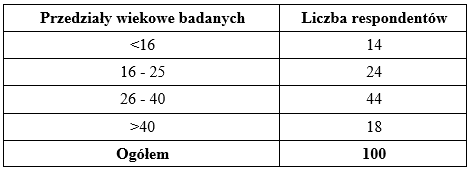
\includegraphics[width=0.75\textwidth]{images/twiek.PNG}
  \caption{Wiek osób biorących udział w badaniu.}
  \caption*{Źródło: opracowanie własne.}
  \label{tbl:twiek}
\end{table}

W tabeli \ref{tbl:twyksztalcenie} zilustrowany jest podział respondentów względem wykształcenia. Najwięcej osób, które udzieliły odpowiedzi posiadają wykształcenie wyższe (54\%). Osoby z wykształceniem średnim i podstawowym stanowią kolejno 26\% oraz 9\%. Pozostałe wykształcenie, opisane jako inne posiadało 11\% badanych.

\clearpage

\begin{table}[htb]
  \centering
  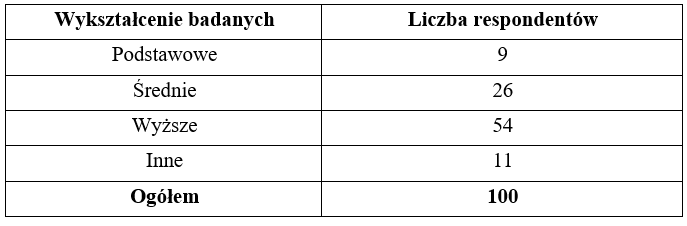
\includegraphics[width=0.85\textwidth]{images/twyksztalcenie.PNG}
  \caption{Wykształcenie osób biorących udział w badaniu.}
  \caption*{Źródło: opracowanie własne.}
  \label{tbl:twyksztalcenie}
\end{table}

Na tym etapie zbadano liczbę osób, które miały doświadczenie z grami VR jak i grami wideo. Odrzuceni zostali respondenci, którzy nie mieli styczności z żadną z platform. Większość z osób, bo aż 93\% korzystało z obu platform, osób korzystających tylko z gier VR było 2\%, a tylko gier wideo 5\%, co ukazuje rysunek \ref{figure:dplatformy}.

\begin{figure}[htb]
  \centering
  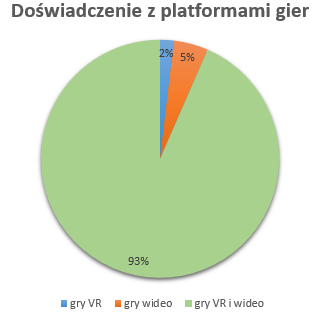
\includegraphics[width=0.6\textwidth]{images/dplatformy.PNG}
  \caption{Doświadczenie z platformami gier osób biorących udział w badaniu.}
  \caption*{Źródło: opracowanie własne.}
  \label{figure:dplatformy}
\end{figure}

\clearpage

\section{Wyniki}

\subsection{Wiek gracza a ulubiona platforma}

Gry wideo jako ulubione medium wybrało 49\% ankietowanych, natomiast gry VR 51\%. Podział ten jednak nie jest tak równomierny w odniesieniu to wieku graczy, co ilustruje rysunek \ref{figure:dwiek}.

\begin{figure}[htb]
  \centering
  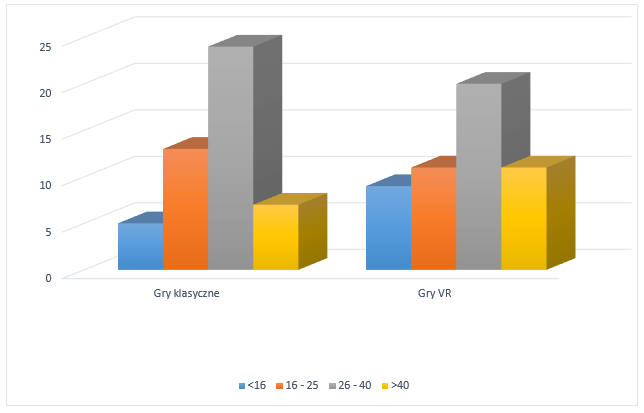
\includegraphics[width=0.9\textwidth]{images/dwiek.PNG}
  \caption{Podział wiekowy użytkowników względem ulubionej platformy.}
  \caption*{Źródło: opracowanie własne.}
  \label{figure:dwiek}
\end{figure}

Z rysunku \ref{figure:dwiek}  wynika, że najmłodsza jak i najstarsza grupa (poniżej 16 oraz powyżej 40 roku życia) badanych preferuje rozgrywkę w trybie VR, natomiast osoby z przedziału wiekowego 16-40 wybierają częściej rozgrywkę w postaci gier wideo. 

\subsection{Czas jednej rozgrywki}

Dane ukazane w tabeli \ref{tbl:tczas} przedstawiają, że czas poświęcony na jedną sesję grania w gry VR, a gry wideo znacząco się różni. W przypadku VR 38\% osób poświęca na grę mniej niż jedną godzinę, a aż 49\% 1 - 2 godzin. Odpowiedź 2 - 5 godzin zaznaczyło 13\%. Żaden z korespondentów nie odpowiedział, że poświęca średnio podczas jednej sesji więcej niż 5 godzin.

Natomiast w przypadku grania w gry wideo, czas poświęcony na jedną sesję, która wynosi mniej niż godzinę to 15\%, a 1 - 2 godzin 33\%. Największy odsetek graczy poświęca na jedną sesję 41\%, a 10\% odpowiadających gra jednorazowo powyżej 5 godzin. 

\clearpage

\begin{table}[htb]
  \centering
  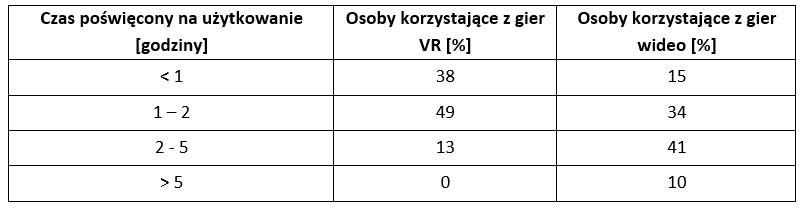
\includegraphics[width=0.8\textwidth]{images/tczas.PNG}
  \caption{Czas poświęcony na użytkowanie przez graczy danej platformy podczas jednej sesji.}
  \caption*{Źródło: opracowanie własne.}
  \label{tbl:tczas}
\end{table}

\subsection{Częstotliwość grania}

Podobna różnorodność jak w przypadku czasu jednej rozgrywki występuje w porównaniu częstotliwości grania w gry VR i gry wideo. Osoby grające rzadziej niż raz w miesiącu stanowią 30\% w przypadku korzystania z technologii VR, oraz 9\% w przypadku korzystania z gier wideo. Wybór przedziału w postaci 1 - 4 razy w miesiącu dokonało kolejno: dla VR 55\%, co było najczęściej wybieraną odpowiedzią, a dla gier wideo 34\%. Kilka razy w tygodniu natomiast z VR korzysta 14\% graczy, a aż 47\% z gier wideo. Najmniej osób odpowiedziało, że gra codziennie w VR (1\%) oraz w gry wideo (11\%).

\begin{table}[htb]
  \centering
  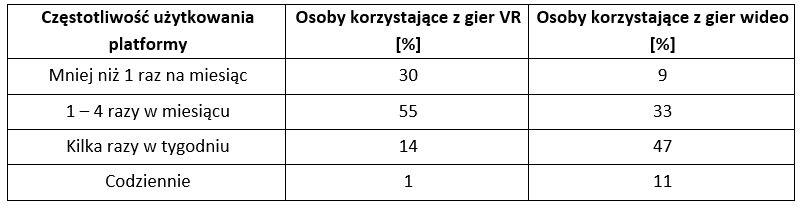
\includegraphics[width=0.9\textwidth]{images/tczestotliwosc.PNG}
  \caption{Częstotliwość użytkowania danej platformy przez graczy.}
  \caption*{Źródło: opracowanie własne.}
  \label{tbl:tczestotliwosc}
\end{table}

\subsection{Immersja a zmęczenie}

Pomimo tego, że respondenci podzielili się na dwie równe grupy jeśli chodzi o preferencje platformy (VR 51\% oraz gry wideo 49\%) to w pytaniach dotyczących wywołania zmęczenia przez grę oraz zdolności gry do pochłonięcia uwagi gracza i wywołania silnych emocji, większość była zgodna. Wyniki tego zestawienia przedstawia tabela \ref{tbl:tzmeczenie}.

\begin{table}[htb]
  \centering
  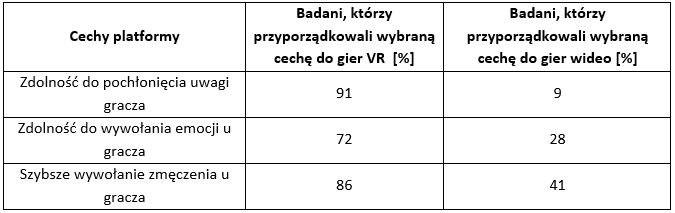
\includegraphics[width=0.9\textwidth]{images/tzmeczenie.PNG}
  \caption{Przyporządkowanie określonych cech do jednej z platform przez ankietowanych.}
  \caption*{Źródło: opracowanie własne.}
  \label{tbl:tzmeczenie}
\end{table}

\subsection{Zdolność platformy do wywołania specyficznych emocji a poziom jej pożądania przez graczy}

Tabela \ref{tbl:tpredyspozycje} wyłania najbardziej i najmniej pożądaną emocję wśród graczy, a także ukazuje predyspozycje gier VR oraz gier wideo do wywołania konkretnych emocji.

\begin{table}[htb]
  \centering
  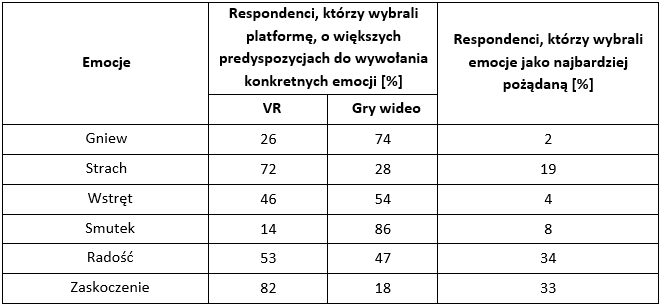
\includegraphics[width=0.8\textwidth]{images/tpredyspozycje.PNG}
  \caption{Emocje i predyspozycje danej platformy do łatwości jej wywołania oraz ważność konkretnej emocji dla graczy.}
  \caption*{Źródło: opracowanie własne.}
  \label{tbl:tpredyspozycje}
\end{table}

Najbardziej pożądaną emocją wśród respondentów okazuje się radość, którą wybrało 34\%. Kolejno były to: zaskoczenie(33\%), strach(19\%), smutek(8\%), wstręt(4\%), gniew(2\%).


Ankietowani wybierali platformę, która ma według nich większe predyspozycje do wywołania konkretnych emocji. Z ankiety wynika, że przy użyciu VR łatwiej wywołać takie emocje jak: zaskoczenie(82\%), strach(72\%) oraz radość(53\%), jednak to gry wideo mają większe predyspozycje do wywołania takich emocji jak: gniew(74\%), wstręt(54\%), smutek(86\%). 

\subsection{Ulubione gatunki gier i ich elementy}

Ulubione gatunki uczestników ankiety przedstawia rysunek \ref{fig:dgatunek}. Większość respondentów za ulubiony gatunek gier wybrało gry zręcznościowe (31\%). Później kolejno: gry sportowe i symulacyjne (29\%), gry przygodowe i fabularne (23\%). Najmniej respondentów uważa za swój ulubiony gatunek gry strategiczne (17\%).

\begin{figure}[htb]
  \centering
  \includegraphics[width=0.8\textwidth]{images/dgatunek.PNG}
  \caption{Ulubione gatunki gier wybrane przez graczy.}
  \caption*{Źródło: opracowanie własne.}
  \label{fig:dgatunek}
\end{figure}

\clearpage

Najbardziej znaczącym elementem rozgrywki dla respondentów okazało się ``wyzwanie, rywalizacja i osiągnięcie sukcesu'' - odpowiedziało tak 43\% ankietowanych, najmniej znaczącym elementem (12\%) zostało ``zaangażowanie ciała w rozgrywkę''. ``doświadczenie społeczne'' oraz ``fabuła, historia, wpływ na jej losy'' są najważniejszym elementem dla podobnej liczby graczy bo kolejno: 22\% i 23\%, co przedstawia tabela \ref{tbl:telementy}.

\begin{table}[htb]
  \centering
  \includegraphics[width=0.8\textwidth]{images/telementy.PNG}
  \caption{Najbardziej znaczące elementy rozgrywki dla graczy.}
  \caption*{Źródło: opracowanie własne.}
  \label{tbl:telementy}
\end{table}

\subsection{Wady i zalety obu platform}

Respondenci w pytaniach otwartych udzielili odpowiedzi na pytanie jakie są wady i zalety obu platform. Na podstawie najczęściej występujących odpowiedzi stworzona została tabela  \ref{tbl:twadyzalety}.

\begin{table}[htb]
  \centering
  \includegraphics[width=1\textwidth]{images/twadyzalety.PNG}
  \caption{Najczęściej wymieniane wady i zalety gier VR i gier wideo przez respondentów.}
  \caption*{Źródło: opracowanie własne.}
  \label{tbl:twadyzalety}
\end{table}

   

% WNIOSKI !!!!!!!!!!!!!!!!!!!!!!!!!!!!!!!!!
    
    
\section{Wnioski}

\subsection{Preferencje graczy}

Analizując dane na temat wieku oraz preferencji co do ulubionej platformy, zauważalny jest znaczny podział na dwie grupy. Osoby najmłodsze jak i najstarsze preferują rozgrywkę w formie VR, natomiast osoby w wieku 16-40 wybierają gry wideo. Dane z ankiety pochodzą z roku 2020, więc osoby te urodziły się w latach 1980-2004. Spora część osób będących w tym przedziale swoją młodość spędzała w latach, kiedy dużą popularnością cieszyły się gry arcade, gry komputerowe oraz konsolowe, czyli te występujące po tzw. złotej erze gier arcade - lata 80,90 XX wieku oraz na początku XXI wieku.  Można wywnioskować, że osoby te miały styczność z grami w latach młodości, co pozwoliło im na obycie się z różnego typu sprzętem i wyrobiło pewne umiejętności, które przydają się w erze dzisiejszych gier wideo. Kolejną kwestią może być przyzwyczajenie użytkowników do tego typu gier. Osoby młode, czyli te poniżej 16 lat oraz osoby powyżej 40 lat mogły nie mieć okazji aby zainteresować się grami wideo. Można zauważyć, że te osoby często wybierają rozrywkę w trybie VR lub tą, dostarczaną przez urządzenia mobilne - głównie telefony typu smartfon. Potwierdzają to także odpowiedzi w pytaniach otwartych, gdzie jedną z częściej wymienianych zalet VR jest intuicyjność. Próg wejścia dla młodych graczy oraz starszych osób jeśli chodzi o gry wideo nie jest tak niski jak w przypadku gier VR.

Osoby korzystające z obu platform najczęściej wybierają gry zręcznościowe, sportowe oraz symulacyjne, a większość ankietowanych wybrało ``Wyzwanie, rywalizację i osiągnięcie sukcesu'' jako najbardziej znaczący element rozgrywki. Dowodzi to, że osoby korzystające zarówno z VR jak i gier wideo mają podobne preferencje co do gatunku gier, jak i cenią w grach podobne elementy rozgrywki. Ma to związek z tym, że gry VR polegają najczęściej na rywalizacji poprzez proste czynności, lecz bez skomplikowanej fabuły. Na podstawie danych z tabeli \ref{tbl:twadyzalety} można stwierdzić, że gry VR najczęściej wybierane są ze względu na intuicyjność, prostotę oraz formę zabawy, przeciwstawnie do gier wideo, gdzie gracze głównie oczekują rozbudowanej rozgrywki z dobrą oprawą graficzną. Można wysnuć wniosek, że preferencje graczy znacznie się różnią - część z nich zależy od konkretnych cech użytkownika, inne natomiast to kwestia zainteresowań lub upodobań.


\subsection{Charakter rozgrywki}

VR charakteryzuje się dużą zdolnością do wywołania emocji oraz bardzo łatwo pochłania uwagę gracza. Analizując dane wykryto zależność między kilkoma czynnikami:
\begin{itemize}
  \item zdolnością VR do pochłonięcia uwagi gracza,
  \item zdolnością VR do wywołania emocji,
  \item częstotliwością grania,
  \item czasem grania.
\end{itemize}

Spoglądając na dane, można stwierdzić, że osoby korzystające z VR najczęściej poświęcają na grę maksymalnie 2 godziny podczas jednej sesji, która odbywa się od 1 do 4 razy w miesiącu. Inny charakter ma korzystanie z gier wideo - kiedy to pojedyncza sesja trwa najczęściej od 2 do 5 godzin i jest odbywana kilka razy w tygodniu. Analizując te dane można zauważyć pewną zależność - zdolność gier do dużej immersji prowadzi do wywołania silnych emocji, co z kolei negatywnie skutkuje zmęczeniem fizycznym oraz psychicznym po krótkiej rozgrywce, dlatego osoby sięgają po gry VR rzadziej jak i na krótszy czas. Gry wideo z kolei są mniej męczące, bardziej komfortowe i pozwalają na częstszą i dłuższą rozgrywkę. Gry wideo z reguły dostarczają mniej intensywnych przeżyć niż gry VR, ale pozwalają na większy relaks i odpoczynek. 

\subsection{Predyspozycje platform do wywołania specyficznych emocji u użytkownika}

%OLD  

% Zarówno gry VR jak i gry wideo są dobrym sposobem na wywołanie emocji u swoich użytkowników. Większość z ankietowanych odpowiedziało, że zdolność gier do wywołania określonych stanów emocjonalnych jest dla nich bardzo ważna. VR dzięki swoim cechom ma dużą zdolność do wywołania emocji podczas rozgrywek lecz ze względu na początkowe stadium rozwoju tej technologii w porównaniu do gier wideo nie ma ona tak dużo zwolenników. Z ankiety wynika, że to VR ma większe predyspozycje do wywołania najbardziej pożądanych emocji przez graczy (radość, zaskoczenie, strach) lecz nie jest tak popularną formą rozrywki jak gry wideo. Aktualne liczbę graczy ogółem na świecie szacuje się na ponad 2.5 miliarda, z czego gracze VR to tylko 171 milionów\citep{website:gameindustry, website:vrstats}. Liczba ta ciągle rośnie, a to za sprawą wciąż rozwijającej się technologii VR. Największą zmorą VR jest brak "pełnoprawnych" gier, lecz i to ulega zmianie. Wydanie jednej, dobrze przyjętej przez graczy produkcji może znacząco zmienić liczbę aktywnych graczy. Przykładem może być wydanie gry "Half-Life: Alyx", kiedy  w ciągu jednego miesiąca odnotowano przyrost 1 miliona nowych użytkowników VR\citep{website:alyx}.

%  NEW

% Technologia VR pozwala na wywołanie silnych i intensywnych emocji u swoich
% użytkowników, lecz niesie to za sobą także negatywne skutki, stad wiele osób wybiera
% klasyczne gry wideo. Zestawiając obie formy użytkowania gier (tj. wideo i VR) oraz biorąc
% pod uwagę emocjonalność gracza możemy wyodrębnić wiele zalet i wad, które wpływają na
% wywoływanie danego afektu u użytkownika. Wybór platformy zależy w głównej mierze od
% tego, jakiego rodzaju rozrywki oczekuje użytkownik. Intensywność wywołanych emocji, ich
% nacechowanie oraz sposób rozgrywki znacząco się różni w przypadku obu platform stąd
% porównywanie, która z nich jest lepsza wydaje się być bezcelowe. Gry VR często występują
% w nieskomplikowanych formach, aniżeli jako pełnoprawny produkt konsumencki. Jednym z
% wyjątków jest wymieniony wielokrotnie w pracy ‘Half Life Alyx’, który można nazwać
% faktyczną pełnoprawną wersją gry VR. Jak zostało opisane w tekście, każda forma wpływa na
% inny rodzaj emocji. Tak samo postrzegają to ankietowani, wg których znaczną przewagę nad
% wywoływaniem m.in. zaskoczenia ma technologia VR.

%  NEW NEW

Zarówno gry VR jak i gry wideo są dobrym sposobem na wywołanie emocji u swoich użytkowników. Większość z ankietowanych odpowiedziało, że zdolność gier do wywołania określonych stanów emocjonalnych jest dla nich bardzo ważna. Najbardziej pożądanymi emocjami są kolejno: radość, zaskoczenie i strach. Najmniej natomiast: gniew wstręt oraz smutek. 

VR dzięki swoim cechom ma dużą zdolność do wywołania emocji podczas rozgrywek lecz ze względu na początkowe stadium rozwoju tej technologii w porównaniu do gier wideo nie ma ona tak dużo zwolenników. Technologia VR pozwala na wywołanie silnych i intensywnych emocji u swoich
użytkowników, lecz niesie to za sobą także negatywne skutki (zmęczenie psychiczne i fizyczne oraz symptomy choroby wirtualnej rzeczywistości - podobne do choroby lokomocyjnej), stąd wiele osób wybiera klasyczne gry wideo.

Z ankiety wynika, że to VR ma większe predyspozycje do wywołania najbardziej pożądanych emocji przez graczy (radość, zaskoczenie, strach) lecz nie jest tak popularną formą rozrywki jak gry wideo. Zauważyć więc można związek między platformą a rodzajem emocji które wywołuje. VR znacząco lepiej radzi sobie z wywołaniem zaskoczenia oraz strachu w porównaniu do gier wideo, które z kolei lepiej radzą sobie z wywołaniem smutku u graczy. Predyspozycje platform do wywołania radości i wstrętu są bardzo zbliżone, natomiast większość badanych wybrało gry wideo jako platformę mającą większą zdolność do wywołania gniewu. Analizując dane wywnioskować można, że chociaż nie wszystkie emocje są nacechowane pozytywnie, są one pożądane przez graczy. Tymi, które są najważniejsze dla graczy to kolejno: radość, zaskoczenie i strach, a te najmniej pożądane to gniew wstręt oraz smutek. Na podstawie analizy można wywnioskować, że wywołanie emocji przez gry jest pożądane z perspektywy gracza oraz można stwierdzić, że każda z platform operuje specyficznymi zdolnościami do wywołania określonych emocji. 


% % STARE !!!!!!!!!!!!!!!!!!!!!!

% \subsection{Cechy gracza}

% Analizując dane na temat wieku oraz preferencji co do ulubionej platformy, zauważalny jest znaczny podział na dwie grupy. Osoby najmłodsze jak i najstarsze preferują rozgrywkę w formie VR, natomiast osoby w wieku 16-40 wybierają gry wideo. Dane z ankiety pochodzą z roku 2020, więc osoby te urodziły się w latach 1980-2004. Spora część osób będących w tym przedziale swoją młodość spędzała w latach, kiedy dużą popularnością cieszyły się gry arcade, gry komputerowe oraz konsolowe, czyli te występujące po tzw. złotej erze gier arcade - lata 80,90 XX wieku oraz 00 XXI wieku.  Można wywnioskować, że osoby te miały styczność z grami w latach młodości, co pozwoliło im na obycie się z różnego typu sprzętem i wyrobiło pewne umiejętności, które przydają się w erze dzisiejszych gier wideo. Kolejną kwestią może być przyzwyczajenie użytkowników do tego typu gier. Osoby młode, czyli te poniżej 16 lat oraz osoby powyżej 40 lat mogły nie mieć okazji aby zainteresować się grami wideo. Można zauważyć, że te osoby często wybierają rozrywkę w trybie VR lub tą, dostarczaną przez urządzenia mobilne - głównie telefony typu smartfon. Potwierdzają to także odpowiedzi w pytaniach otwartych, gdzie jedną z częściej wymienianych zalet VR jest intuicyjność. Próg wejścia dla młodych graczy oraz starszych osób jeśli chodzi o gry wideo nie jest tak niski jak w przypadku gier VR.


% \subsection{Immersja}

% VR charakteryzuje się dużą zdolnością do wywołania emocji oraz bardzo łatwo pochłania uwagę gracza. Analizując dane wykryto zależność między kilkoma czynikami:

% \begin{itemize}
%   \item zdolnością VR do wywołania emocji,
%   \item częstotliwością grania,
%   \item czasem grania.
% \end{itemize}

% Spoglądając na dane, można stwierdzić, że osoby korzystające z VR najczęściej poświęcają na grę maksymalnie 2 godziny podczas jednej sesji, która odbywa się od 1 do 4 razy w miesiącu. Inny charakter ma korzystanie z gier wideo - kiedy to pojedyncza sesja trwa najczęściej od 2 do 5 godzin, i jest odbywana kilka razy w tygodniu. Analizując te dane można zauważyć pewną zależność - zdolność gier do dużej immersji prowadzi do wywołania silnych emocji, co z kolei negatywnie skutkuje zmeczęniem fizycznym oraz psychicznym po krótkiej rozgrywce dlatego osoby sięgają po gry VR rzadziej jak i na krótszy czas. Gry wideo z kolei są mniej męczące, bardziej komfortowe i pozwalają na częstszą i dłuższą rozgrywkę. Gry wideo z reguły dostarczają mniej intensywnych przeżyć niż gry VR ale pozwala to na większy relaks i odpoczynek. 


% \subsection{Emocje jako czynnik sukcesu}

% Zarówno gry VR jak i gry wideo są dobrym sposobem na wywołanie emocji u swoich użytkowników.VR dzięki swoim cechom ma dużą zdolność do wywołania emocji podczas rozgrywek lecz ze względu na początkowe stadium rozwoju tej technologii w porównaniu do gier wideo nie ma ona tak dużo zwolenników. Z ankiety wynika, że to VR ma większe predyspozycje do wywołania najbardziej pożądanych emocji przez graczy (z reguły tych pozytywnych) lecz nie jest tak popularną formą rozrywki jak gry wideo. Większość z ankietowanych odpowiedziało, że zdolność gier do wywołania określonych stanów emocjonalnych jest dla nich ważna lub najważniejsza.

% Aktualne liczbę graczy ogółem na świecie szacuje się na ponad 2.5 miliarda, z czego gracze VR to tylko 171 milionów\citep{website:gameindustry, website:vrstats}. Liczba ta ciągle rośnie, a to za sprawą wciąż rozwijającej się technologii VR. Największą zmorą VR jest brak "pełnoprawnych" gier, lecz i to ulega zmianie. Wydanie jednej, dobrze przyjętej przez graczy produkcji może znacząco zmienić liczbę aktywnych graczy. Przykładem może być wydanie gry "Half-Life: Alyx", kiedy  w ciągu jednego miesiąca odnotowano przyrost 1 miliona nowych użytkowników VR\citep{website:alyx}.

% \subsection{Preferencje użytkownika a wybór platformy}

% Granie w gry VR znacząco rózni się od klasycznej rozgrywki. Na podstawie najczęściej występujących odpowiedzi badanych na temat wad i zalet obu platform stworzona została tabela zaprezentowana poniżej.

% \begin{table}[htb]
%   \centering
%   \includegraphics[width=0.8\textwidth]{images/twadyzalety.PNG}
%   \caption{Najczęściej wymieniane wady i zalety przez ankietowanych}
%   \caption*{Źródło: opracowanie własne}
%   \label{tbl:twadyzalety}
% \end{table}

% % Wybór platformy i gatunku gier zależy w głównej mierze od tego, jakiego rodzaju rozrywki oczekuje użytkownik. Intensywność wywołanych emocji, ich nacechowanie oraz sposób rozgrywki znacząco się różni w przypadku obu platform stąd porównywanie, która z nich jest lepsza wydaje się być bezcelowym. Gry wideo mają inny charakter niż gry VR, które z kolei po pewnym czasie stają się męczące i monotonne - polegają najczęsciej na prostych czynnościach, bez skompliokwanaje fabuły. Rynek VR wciąż ewoluuje i producenci gier coraz częściej będą tworzyć coraz bardziej zaawansowane dzieła, czego przykładem może być wcześniej wymieniony "Half-Life: Alyx".

% \chapter*{Zakończenie}
\label{chap:zakonczenie}
\addcontentsline{toc}{chapter}{Zakończenie}


Celem pracy było opisanie czytelnikowi czym jest technologia VR,
omówienie procesu powstania emocji oraz narzędzi wykorzystywanych do ich wywołania w
grach oraz zbadanie, jakimi zdolnościami do wywołania konkretnych emocji cechują się gry VR oraz gry wideo.
    
W pierwszym rozdziale pracy zdefiniowano technologię wirtualnej rzeczywistości jako połączenie sprzętu i oprogramowania, które tworzy całkowicie nowe, cyfrowe symulacje. VR składa się z trzech głównych części jakimi są:  immersja, wyobraźnia, interakcja. W tym rozdziale została także opisana historia VR: od początków sięgających ściennych malowideł po lata współczesne, skupiające się głównie na rozrywce VR, ale także zostały podane prognozy na przyszłość mówiące o jej nowych zastosowaniach.

W kolejnym rozdziale przybliżono pojęcie emocji jako stanu umysłu, któremu towarzyszą zmiany somatyczne, akty ekspresji i działania. Dokonano  klasyfikacji emocji na funkcjonalne jak i niefunkcjonalne oraz omówiono proces powstania emocji dzieląc go na 4 składowe jakimi są: 
``ocena poznawcza'', ``wartościowanie kontekstowe'', ``gotowość do działania'' i ``zmiany psychologiczne, ekspresja, działanie''.

Trzeci rozdział poświęcony został na ukazanie związku emocji z grami. W tym celu przywołano 6 podstawowych emocji jakimi są: gniew, strach, wstręt, radość, smutek oraz zaskoczenie. Zdefiniowano grę jako aktywne medium, które jest rozróżnialne od pasywnych (np. filmów) dzięki swojej głównej właściwości jaką jest interaktywność. Wymieniono charakteryzujące gry atrybuty, które pozwalają na wywołanie emocji: użycie awatara, interaktywność, kontrolę, poczucie sprawczości, symulowane akcje, interaktywny dyskomfort, wyzwanie, doświadczenie społeczne, zaangażowanie ciała.

W ostatnim rozdziale zaprezentowano i przedyskutowano wyniki badań. Przeprowadzone badania pokazały, że preferencje graczy w stosunku do ulubionej platformy znacznie się różnią w zależności od wieku - najmłodsi i najstarsi gracze preferują rozrywkę w trybie VR, natomiast osoby w wieku od 16 do 40 lat wybierają rozrywkę w formie gier wideo. Gracze wybierają najczęściej gry zręcznościowe, sportowe oraz symulacyjne, a ich ulubioną częścią rozgrywki jest najczęściej element wyzwania, rywalizacji i osiągnięcia sukcesu. Rozgrywka graczy różni się znacząco w zależności od wybranej platformy. Osoby korzystające z gier VR odbywają krótkie sesje o małej częstotliwości z powodu negatywnych skutków, jakie powoduje częste i długie korzystanie z gogli wirtualnej rzeczywistości, natomiast osoby korzystające z gier wideo grają częściej i dłużej ze względu na bardziej relaksujący charakter rozgrywek. Pomimo że obie platformy mają dobre predyspozycje do wywołania emocji wśród graczy, to dzięki większej zdolności do pochłonięcia uwagi gracza, lepiej radzi sobie z tym technologia VR. Zauważalny jest także związek pomiędzy platformą a rodzajem emocji, które wywołuje. VR znacząco lepiej radzi sobie z wywołaniem zaskoczenia oraz strachu w porównaniu do gier wideo, które z kolei lepiej radzą sobie z wywołaniem smutku u graczy. Predyspozycje platform do wywołania radości i wstrętu są podobne, natomiast większość badanych wybrało gry wideo jako platformę mającą większą zdolność do wywołania gniewu. Analizując dane wywnioskować można, że chociaż nie wszystkie emocje są nacechowane pozytywnie, są one pożądane przez graczy. Tymi, które są najważniejsze dla graczy to kolejno: radość, zaskoczenie i strach, a te najmniej pożądane to gniew wstręt oraz smutek. 

Gry VR przechodzą powolną transformacje i w przyszłości spodziewać się będzie
można, że zostaną rywalem gier wideo oraz stanowić będą coraz to większą część rynku
gier. Intensywność wywołanych emocji, ich nacechowanie oraz sposób rozgrywki znacząco się różni w przypadku obu platform stąd porównywanie, która z nich jest lepsza wydaje się być bezcelowe ponieważ każda z nich ma na celu dostarczenie innych wrażeń użytkownikowi. Wnioski takie można wysunąć również na podstawie odpowiedzi ankietowanych, co potwierdza, że technologia VR jest pożądana, nie tylko jako forma rozrywki, ale także w dziedzinach naukowych. Pomocne w tej kwestii jest finansowe ugruntowanie technologii VR i rynku, na
którym głównie bazuje. Przewidywania te jednak mogą również odwoływać się do gier
wideo, które rozwijają się w ogromnym tempie i spotykają się z niezwykle pozytywny
odbiorem wśród coraz to większej populacji graczy. Możemy zatem stwierdzić, że niezależnie od formy, gry VR i
gry wideo są niezastąpionym sposobem rozrywki, spędzania wolnego czasu oraz przeżywania
wirtualnych przygód.


% Technologia VR pozwala na wywołanie silnych i intensywnych emocji u swoich
% użytkowników, lecz niesie to za sobą także negatywne skutki, stad wiele osób wybiera
% klasyczne gry wideo. Zestawiając obie formy użytkowania gier (tj. wideo i VR) oraz biorąc
% pod uwagę emocjonalność gracza możemy wyodrębnić wiele zalet i wad, które wpływają na
% wywoływanie danego afektu u użytkownika. Wybór platformy zależy w głównej mierze od
% tego, jakiego rodzaju rozrywki oczekuje użytkownik. Intensywność wywołanych emocji, ich
% nacechowanie oraz sposób rozgrywki znacząco się różni w przypadku obu platform stąd
% porównywanie, która z nich jest lepsza wydaje się być bezcelowe. Gry VR często występują
% w nieskomplikowanych formach, aniżeli jako pełnoprawny produkt konsumencki. Jednym z
% wyjątków jest wymieniony wielokrotnie w pracy ‘Half Life Alyx’, który można nazwać
% faktyczną pełnoprawną wersją gry VR. Jak zostało opisane w tekście, każda forma wpływa na
% inny rodzaj emocji. Tak samo postrzegają to ankietowani, wg których znaczną przewagę nad
% wywoływaniem m.in. zaskoczenia ma technologia VR.

% % bibliografia
% \newpage
% \bibliographystyle{apalike}
% \bibliography{bibliography} 
 
% % spis tabel
% \newpage
% \listoftables

% % spis rysunków
% \newpage
% \listoffigures

% % dodatek, załącznik
% \include{apalike}
% \chapter*{Ankieta}
\label{chap:dodatek}
\addcontentsline{toc}{chapter}{Ankieta}
\addtocounter{chapter}{0}

\begin{figure}[h]
	\centering
	\includegraphics[width=0.7\textwidth]{images/ankieta1.PNG}
\end{figure}
\begin{figure}
	\centering
	\includegraphics[width=0.7\textwidth]{images/ankieta12.PNG}
\end{figure}
\begin{figure}
	\centering
	\includegraphics[width=0.7\textwidth]{images/ankieta123.PNG}
\end{figure}
\begin{figure}
	\centering
	\includegraphics[width=0.7\textwidth]{images/ankieta1234.PNG}
\end{figure}
\begin{figure}
	\centering
	\includegraphics[width=0.7\textwidth]{images/ankieta12345.PNG}
\end{figure}
\begin{figure}
	\centering
	\includegraphics[width=0.7\textwidth]{images/ankieta123456.PNG}
\end{figure}


% \end{document}
